\documentclass[11pt,a4paper,openany]{ctexrep}
\usepackage[a4paper,margin=23mm,headheight=15pt]{geometry}
\usepackage{amsmath,amssymb,mathtools,bm}
\usepackage{siunitx}
\usepackage{booktabs,tabularx,array,longtable}
\usepackage{enumitem}
\usepackage{graphicx}
\usepackage{xcolor}
\usepackage{tikz}
\usepackage{pgfplots}
\pgfplotsset{compat=1.18}
\usetikzlibrary{arrows.meta,positioning,shapes.geometric,calc,fit,decorations.pathmorphing}
\usepackage[most]{tcolorbox}
\usepackage{hyperref}
\usepackage{fancyhdr}
\usepackage{titlesec}
\usepackage{microtype}
\usepackage{setspace}

\definecolor{KidBlue}{HTML}{22577A}
\definecolor{KidTeal}{HTML}{2A9D8F}
\definecolor{KidGold}{HTML}{E9C46A}
\definecolor{KidRed}{HTML}{C8553D}
\definecolor{KidGray}{HTML}{F3F5F7}
\definecolor{KidDark}{HTML}{263238}

\hypersetup{colorlinks=true,linkcolor=KidBlue,urlcolor=KidBlue,citecolor=KidTeal,pdftitle={KID入门讲义 v0.10 Step 4 Formula Pedagogy Preview},pdfauthor={KID Intro Guide project}}
\setstretch{1.15}
\setlist[itemize]{leftmargin=2em,itemsep=0.25em,topsep=0.4em}
\setlist[enumerate]{leftmargin=2em,itemsep=0.25em,topsep=0.4em}
\setlength{\parindent}{2em}
\setlength{\parskip}{0.25em}

\pagestyle{fancy}
\fancyhf{}
\fancyhead[L]{KID 入门讲义 v0.10 Step 4 Formula Pedagogy Preview}
\fancyhead[R]{\leftmark}
\fancyfoot[C]{\thepage}
\renewcommand{\headrulewidth}{0.4pt}

\titleformat{\chapter}[display]{\bfseries\Huge\color{KidDark}}{\filleft\color{KidBlue}\fontsize{44}{44}\selectfont\thechapter}{1ex}{\titlerule\vspace{1ex}\filright}
\titleformat{\section}{\Large\bfseries\color{KidBlue}}{\thesection}{0.7em}{}
\titleformat{\subsection}{\large\bfseries\color{KidTeal}}{\thesubsection}{0.7em}{}
\titleformat{\part}[display]
  {\centering\bfseries\Huge\color{KidDark}}
  {\color{KidBlue}\Large Part~\thepart}
  {1.2ex}
  {\titlerule[1.2pt]\vspace{1.4ex}}
\titlespacing*{\part}{0pt}{0pt}{0pt}

\newtcolorbox{goalbox}{colback=KidBlue!5,colframe=KidBlue,boxrule=0.8pt,arc=2mm,title=本节目标,fonttitle=\bfseries}
\newtcolorbox{intuitionbox}{colback=KidTeal!6,colframe=KidTeal,boxrule=0.8pt,arc=2mm,title=物理直觉,fonttitle=\bfseries}
\newtcolorbox{projectbox}{colback=KidGold!16,colframe=KidGold!80!black,boxrule=0.8pt,arc=2mm,title=工程案例：150 GHz 双偏振 LEKID,fonttitle=\bfseries}
\newtcolorbox{mistakebox}{colback=KidRed!5,colframe=KidRed,boxrule=0.8pt,arc=2mm,title=常见误区,fonttitle=\bfseries}
\newtcolorbox{checkpointbox}{colback=KidGray,colframe=KidDark!55,boxrule=0.7pt,arc=2mm,title=理解检查,fonttitle=\bfseries}
\newtcolorbox{formula}[1][]{colback=white,colframe=KidBlue!75,boxrule=0.9pt,arc=1mm,#1}
\newtcolorbox{formulaguidebox}{
  enhanced,breakable,
  colback=KidBlue!2,colframe=KidBlue!55,
  boxrule=0.65pt,arc=2mm,
  title=公式怎么读：不要只背等号,
  fonttitle=\bfseries,
  before skip=0.35em,after skip=0.8em
}
\newcommand{\formulaexplain}[4]{%
\begin{formulaguidebox}
\textbf{\color{KidBlue}数学上：}#1\par
\textbf{\color{KidTeal}物理上：}#2\par
\textbf{\color{KidGold!55!black}工程上：}#3\par
\textbf{\color{KidRed}适用条件：}#4
\end{formulaguidebox}%
}
\newtcolorbox{notebookbox}[1][]{colback=KidGray!45,colframe=KidBlue!55,boxrule=0.8pt,arc=2mm,title=手写练习,fonttitle=\bfseries,#1}
\newtcolorbox{answerbox}[1][]{colback=KidTeal!5,colframe=KidTeal!80!black,boxrule=0.8pt,arc=2mm,title=参考答案,fonttitle=\bfseries,#1}

\newcommand{\chapterguide}[4]{%
\begin{tcolorbox}[
  enhanced,
  breakable,
  colback=KidGray!45,
  colframe=KidBlue!65,
  boxrule=0.8pt,
  arc=2mm,
  title=本章导航,
  fonttitle=\bfseries,
  before skip=0.7em,
  after skip=1.0em]
\renewcommand{\arraystretch}{1.18}
\noindent\begin{tabularx}{\textwidth}{>{\bfseries\color{KidBlue}}p{3.0cm} X}
为什么要学？ & #1 \\
阅读前只需要知道 & #2 \\
读完应能回答 & #3 \\
一句话结论 & \textbf{#4} \\
\end{tabularx}
\end{tcolorbox}%
}

\newcommand{\qp}{\mathrm{qp}}
\newcommand{\Stwentyone}{S_{21}}
\newcommand{\fzero}{f_0}
\newcommand{\Qi}{Q_i}
\newcommand{\Qc}{Q_c}
\newcommand{\Qr}{Q_r}
\newcommand{\Lk}{L_k}
\newcommand{\Lg}{L_g}


% --- Flow-chart conventions ---
% Solid arrows = causal/signal flow; dashed arrows = parameter influence;
% plain lines = structural/reciprocal coupling. Explicit anchors avoid arrow-box collisions.
\tikzset{
  flowbox/.style={draw=KidDark!70,rounded corners=2mm,align=center,minimum height=10mm,inner sep=4pt,font=\small,fill=white},
  flowarrow/.style={-{Stealth[length=2.3mm,width=1.7mm]},line width=0.85pt,draw=KidBlue,shorten <=1.2pt,shorten >=1.2pt},
  goldarrow/.style={-{Stealth[length=2.3mm,width=1.7mm]},line width=0.85pt,draw=KidGold!75!black,shorten <=1.2pt,shorten >=1.2pt},
  influence/.style={-{Stealth[length=2.0mm,width=1.5mm]},dashed,line width=0.7pt,draw=KidTeal!85!black,shorten <=1.0pt,shorten >=1.0pt},
  structlink/.style={line width=0.8pt,draw=KidBlue!85!black},
  dimline/.style={Stealth-Stealth,thin,draw=KidDark!75}
}

\begin{document}

\begin{titlepage}
\centering
\vspace*{2.2cm}
{\fontsize{30}{38}\selectfont\bfseries\color{KidDark} KID 入门讲义}\par
\vspace{0.5cm}
{\Large\color{KidBlue} 从“一个光子”到可读出的微波信号}\par
\vspace{1.4cm}
{\large Version 0.10 Step 4 Formula Pedagogy Preview · 2026-09-10}\par
\vfill
\begin{tcolorbox}[width=0.88\textwidth,colback=KidGray,colframe=KidBlue!55,arc=3mm]
\centering
\large
这不是一本“先学完凝聚态物理再碰器件”的教材。\\[0.5em]
它采用器件设计者视角：\\[0.3em]
\textbf{先建立可运行的物理图景，再逐层补上微观理论、公式、仿真与实验。}
\end{tcolorbox}
\vfill
{\large 面向：毫米/亚毫米波 KID / LEKID 初学与器件设计}\par
\end{titlepage}

\setcounter{tocdepth}{0}% printed TOC: Part + Chapter only
\tableofcontents
\clearpage

\chapter*{如何使用这份讲义}
\addcontentsline{toc}{chapter}{如何使用这份讲义}

这份讲义按“\textbf{物理因果链}”而不是按学科目录组织。第一次阅读时，不要求读者先掌握凝聚态物理、超导微波器件或 KID 专用术语；更推荐先建立一条足够简单的主线，再逐章把每个箭头打开。

\begin{formula}[title=整本书只是在逐层解释这四个箭头]
\[
\boxed{
\text{光}
\rightarrow
\text{超导状态变化}
\rightarrow
\text{谐振器变化}
\rightarrow
\text{微波读出变化}
}
\]
\end{formula}

每一章都尽量回答四个问题：
\begin{enumerate}
  \item \textbf{发生了什么？} —— 先建立可视化的物理图景；
  \item \textbf{为什么？} —— 用最少但必要的公式把直觉固定下来；
  \item \textbf{怎么测？} —— 把物理量连接到真实实验中的 $I/Q$、$S_{21}$、频移和噪声；
  \item \textbf{对器件设计有什么意义？} —— 把材料、几何、电磁仿真和读出重新接回同一条链。
\end{enumerate}

\section*{三条推荐阅读路线}
\begin{tcolorbox}[colback=white,colframe=KidBlue!55,arc=2mm,title=路线 A：完全初学者,fonttitle=\bfseries]
按顺序阅读第 0--10 章。先完成 Part I 的直觉建立，再进入材料、谐振器、噪声和 LEKID 电磁设计。第 11 章属于工程案例，可在第一次通读后再读。
\end{tcolorbox}

\begin{tcolorbox}[colback=white,colframe=KidTeal!65,arc=2mm,title=路线 B：已有 RF / 微波背景,fonttitle=\bfseries]
建议先读第 0--2 章建立 KID 特有因果链，然后优先读第 6 章的 $S_{21}$、IQ circle 与 fitting；再回到第 3--5 章补动能电感与超导材料响应，随后进入第 7--8 章。
\end{tcolorbox}

\begin{tcolorbox}[colback=white,colframe=KidGold!80!black,arc=2mm,title=路线 C：主要目标是 LEKID 仿真与器件设计,fonttitle=\bfseries]
先读第 0--3 章建立器件直觉，再读第 5、8 章理解材料模型与电磁设计；需要把结果写成可复现证据时，再进入第 11 章项目验证矩阵。第 4、6、7 章可作为材料、读出和灵敏度参考。
\end{tcolorbox}

\begin{checkpointbox}
如果某一页突然出现太多陌生符号，不必停下来一次记完。先问：\textbf{这个量位于“光 $\rightarrow$ 超导状态 $\rightarrow$ 谐振器 $\rightarrow$ 微波读出”的哪一个箭头上？} 能回答这一点，就仍然在主线上。
\end{checkpointbox}

\chapter*{符号、缩写与术语速查}
\addcontentsline{toc}{chapter}{符号、缩写与术语速查}

这一节不是要求读者在开始前背诵。它更像一张“路标”：第一次遇到陌生缩写或符号时先来这里查，理解它在整条因果链中的位置，再回正文继续阅读。

\begin{intuitionbox}
本书会保留一些 KID 论文、微波测量和电磁仿真中极常见的英文词，例如 meander、notch、feedline、backshort 和 probe tone。第一次出现时给出中文含义，后文可能直接沿用英文，目的是让教材中的词与论文、VNA/EM 软件界面能够一一对应，而不是要求读者同时记两套术语。
\end{intuitionbox}

\section*{常见缩写}
\small
\noindent\begin{tabularx}{\textwidth}{>{\bfseries\color{KidBlue}}p{1.8cm} p{5.3cm} X}
\toprule
缩写 & 英文全称 & 本书中的含义 \\
\midrule
KID & kinetic inductance detector & 动能电感探测器；利用超导材料的动能电感与损耗变化实现探测。 \\
LEKID & lumped-element kinetic inductance detector & 集总元件 KID；常用 meander 提供吸收/电感、IDC 提供电容。 \\
VNA & vector network analyzer & 矢量网络分析仪；扫频测量复数 $S$ 参数。 \\
ADC & analog-to-digital converter & 模数转换器；把模拟微波读出链的信号变为数字采样。 \\
DDC & digital down conversion & 数字下变频；把每个读出 tone 搬到低速复基带得到 $I(t),Q(t)$。 \\
FDM & frequency-division multiplexing & 频分复用；让大量不同 $f_0$ 的 KID 共用一条读出线。 \\
NEP & noise-equivalent power & 噪声等效功率；把输出噪声折算回输入光功率后的灵敏度指标。 \\
PSD & power spectral density & 功率谱密度，单位通常含 $/\mathrm{Hz}$。 \\
ASD & amplitude spectral density & 幅度谱密度，等于 PSD 的平方根。 \\
TLS & two-level system & 两能级系统；常用于描述介质缺陷引起的一类低频频率噪声。 \\
\bottomrule
\end{tabularx}
\normalsize

\section*{最常用符号}
\small
\begin{longtable}{>{\bfseries\color{KidBlue}}p{2.2cm} p{4.6cm} p{8.0cm}}
\toprule
符号 & 名称 & 先记住什么 \\
\midrule
\endfirsthead
\toprule
符号 & 名称 & 先记住什么 \\
\midrule
\endhead
$\nu$ & 信号光频率 & 毫米波/亚毫米波光子的频率；光子能量为 $h\nu$。 \\
$h$ & Planck 常数 & 把“频率”连接到“单个光子的能量”。 \\
$T_c$ & 超导临界温度 & 粗略决定能隙尺度；弱耦合 BCS 下 $\Delta(0)\simeq1.764k_BT_c$。 \\
$\Delta$ & 超导能隙 & 本书取单准粒子能隙；最基本的 pair-breaking 阈值是 $h\nu\ge2\Delta$。 \\
$N_{\rm qp}$ & 准粒子数 & 吸收功率增加后通常会上升，是“光”到“材料状态”之间的关键中间量。 \\
$n_s$ & 超流载流子密度 & 越低通常意味着动能电感越大。 \\
$L_g$ & 几何电感 & 主要对应导体周围磁场储能。 \\
$L_k$ & 动能电感 & 来自超导载流子的惯性，是 KID 对材料状态敏感的核心。 \\
$\alpha$ & 动能电感占比 & $\alpha=L_k/(L_g+L_k)$；表示总电感中有多少来自敏感的 $L_k$。 \\
$C$ & 电容 & 与总电感共同决定谐振频率。 \\
$f_0$ & 谐振频率 & $f_0=1/(2\pi\sqrt{LC})$；KID 最重要的可测状态量之一。 \\
$Q_i$ & internal quality factor & 内部品质因数，描述器件内部损耗。 \\
$Q_c$ & coupling quality factor & 耦合品质因数，描述谐振器与 feedline 的耦合。 \\
$Q_r$ & loaded/resonator quality factor & 实际读到的总品质因数，满足 $Q_r^{-1}=Q_i^{-1}+Q_c^{-1}$。 \\
$S_{21}$ & 前向传输系数 & 一个复数；可同时看幅度/相位，也可写成 $I+jQ$。 \\
$I,Q$ & 复基带两分量 & $S_{21}=I+jQ$ 的实部与虚部坐标，不是两个独立探测器。 \\
$P_{\rm abs}$ & 吸收光功率 & 真正进入 absorber 并转化为探测器激发的功率。 \\
$\eta_{\rm pb}$ & pair-breaking efficiency & 吸收能量中有效进入准粒子产生链条的比例参数。 \\
$\tau_{\rm qp}$ & 准粒子寿命 & 决定稳态准粒子数与一部分时间响应带宽。 \\
$\sigma_1,\sigma_2$ & 复电导两部分 & $\sigma_1$ 主要关联耗散，$\sigma_2$ 主要关联感性/超流响应。 \\
$R_{\square,n}$ & 正常态方块电阻 & 薄膜工艺中常用的每方块电阻，可用于估算低温 $L_{k,\square}$。 \\
$Z_s=R_s+jX_s$ & 表面阻抗 & 把有限损耗与感性响应放在同一个复数材料参数里。 \\
\bottomrule
\end{longtable}
\normalsize

\section*{几个容易混淆的词}
\begin{itemize}
  \item \textbf{quasiparticle（准粒子）：}不是“普通电子数量”的简单同义词，而是超导体系的激发态描述；入门阶段先把它看成会同时改变损耗与动能电感的材料状态变量。
  \item \textbf{pair breaking（破对）：}打破 Cooper pair 并产生准粒子激发；最基本能量阈值是 $2\Delta$，不是 $\Delta$。
  \item \textbf{meander（蛇形线/曲折电感）：}在 LEKID 中常同时承担毫米波吸收与 GHz 电感两种职责。
  \item \textbf{notch（传输凹口）：}谐振器从 feedline 抽取/重分配能量后，在 $|S_{21}|$ 扫频曲线上出现的凹陷；它不是“吸收谱”的同义词。
  \item \textbf{probe tone（读出探针）：}放在 GHz 谐振附近、用来询问谐振器状态的微波信号；它与被探测的毫米波/亚毫米波信号不是同一频段。
  \item \textbf{responsivity（响应度）：}输入变化引起多大输出变化，例如 $dx/dP_{\rm abs}$；响应度大不自动等于 NEP 小，还必须同时看噪声。
  \item \textbf{co-pol / cross-pol（同偏振/交叉偏振）：}分别描述目标偏振和正交偏振的响应，必须先写清楚定义和归一化方式再比较数值。
  \item \textbf{backshort（背短路反射结构）：}放在 absorber 后方的反射/匹配结构，用干涉与阻抗匹配提高目标频带吸收；“$\lambda/4$”通常只是设计起点。
\end{itemize}

\begin{checkpointbox}
三个特别值得从一开始就区分的量：\textbf{$\nu$ 是被探测光的频率，$f_0$ 是 GHz 谐振器的谐振频率，$f$ 在噪声谱章节里还会表示 Fourier frequency。} 它们都叫“频率”，但在物理链条中的职责完全不同。
\end{checkpointbox}

\part{先建立 KID 直觉}
\setcounter{chapter}{-1}
\chapter{第一次接触 KID，只需要先知道这些}
\chapterguide
{完全陌生的读者需要先知道“这是什么器件、为什么会有两个频段、最后究竟测什么”，否则后面的公式很容易变成符号堆叠。}
{只需要知道频率、电压、电流以及“电感和电容可以形成谐振”这一层电路直觉；不要求预先学过超导。}
{KID/LEKID 是什么；meander、IDC、feedline 分别做什么；为什么信号光与 GHz 读出可以同时存在；notch 和 IQ 图在测量上代表什么。}
{光负责改变超导谐振器，微波探针负责把这种改变读出来。}

\section{先不看公式：KID 到底在做什么？}
KID 是 kinetic inductance detector（动能电感探测器）的缩写。它的基本思路并不是“让光直接产生一根电线里的电压”，而是先让入射光改变一个超导微波谐振器的状态，再用很弱的微波探针去读取这种改变。

第一次接触时，只需要记住四步：
\begin{center}
\begin{tikzpicture}[node distance=8mm and 7mm]
\node[flowbox,fill=KidGold!22,minimum width=30mm] (a) {入射光\\把能量送入薄膜};
\node[flowbox,fill=KidTeal!10,right=of a,minimum width=33mm] (b) {超导状态改变\\可理解为“材料状态变了”};
\node[flowbox,fill=KidBlue!7,right=of b,minimum width=31mm] (c) {谐振器改变\\$f_0$、损耗发生变化};
\node[flowbox,fill=KidGray,right=of c,minimum width=31mm] (d) {微波读出改变\\$S_{21}$ / $I,Q$};
\draw[goldarrow] (a.east)--(b.west);
\draw[flowarrow] (b.east)--(c.west);
\draw[flowarrow] (c.east)--(d.west);
\end{tikzpicture}
\end{center}

\begin{intuitionbox}
把 KID 暂时想成一只“会被光轻微调音的微波谐振器”。光把它的音高和阻尼改了一点；读出系统并不直接数光子，而是非常精确地测这只谐振器发生了多小的变化。
\end{intuitionbox}

\section{LEKID 又是什么？先认清像元里的三个角色}
LEKID 是 lumped-element kinetic inductance detector（集总元件动能电感探测器）。在常见平面结构里，读者最先需要认出三个部件：
\begin{itemize}
  \item \textbf{meander（蛇形电感/吸收结构）}：在毫米波频段吸收信号，同时在 GHz 谐振器中提供重要的动能电感；
  \item \textbf{IDC（interdigitated capacitor，叉指电容）}：主要提供谐振器所需的电容；
  \item \textbf{feedline（读出传输线）}：把 GHz probe tone 送到像元附近，并把经过谐振器影响后的微波信号送回读出链。
\end{itemize}

\begin{center}
\begin{tikzpicture}[scale=0.95]
\draw[KidBlue,line width=1.4pt] (-5,-2.0)--(5,-2.0);
\node[below,font=\small] at (3.4,-2.0) {feedline：GHz 读出};
\draw[KidBlue!80,line width=0.9pt] (-0.8,-1.65)--(-0.8,-1.15);
\draw[KidBlue!80,line width=0.9pt] (-0.45,-1.65)--(-0.45,-1.15);
\node[right,font=\scriptsize] at (-0.25,-1.4) {耦合区};
\draw[KidDark,line width=1.0pt] (-1.8,-0.8)--(-1.2,-0.8)--(-1.2,0.8)--(-0.8,0.8)--(-0.8,-0.8)--(-0.4,-0.8)--(-0.4,0.8)--(0,0.8)--(0,-0.8)--(0.4,-0.8)--(0.4,0.8)--(0.8,0.8)--(0.8,-0.8)--(1.2,-0.8)--(1.2,0.8)--(1.8,0.8);
\node[above,font=\small] at (0,1.05) {IDC：主要提供 $C$};
\draw[KidTeal!80!black,line width=1.0pt] (1.8,0.8)--(2.4,0.8)--(2.4,1.5)--(2.8,1.5)--(2.8,0.3)--(3.2,0.3)--(3.2,1.5)--(3.6,1.5)--(3.6,0.3)--(4.0,0.3);
\node[above,font=\small,align=center] at (3.2,1.75) {meander：\\absorber + $L_k$};
\draw[-{Stealth[length=3mm]},KidGold!80!black,line width=1.2pt] (3.2,3.0)--(3.2,2.05);
\node[above,font=\small] at (3.2,3.0) {毫米波 / 亚毫米波信号};
\end{tikzpicture}
\end{center}

图只是示意，不对应某个具体像元的尺寸。真正器件的 meander、IDC 和耦合区可以有很多不同几何形式；此处只需要先认清“谁负责吸收、谁提供电容、谁负责读出”。

\section{为什么同一个器件里会同时出现 150 GHz 和几 GHz？}
这是 KID 最容易把初学者绕晕的地方。两种频率承担的是\textbf{完全不同的任务}：
\begin{center}
\begin{tabularx}{0.92\textwidth}{>{\bfseries}p{3.1cm} X X}
\toprule
& 被探测的信号光 & 用于读出的微波 \\
\midrule
典型频率 & 例如 \SI{150}{GHz} & 例如 \SI{1}{GHz}--\SI{5}{GHz} \\
任务 & 把能量沉积进超导薄膜 & 探测谐振器状态有没有变化 \\
直觉 & “改变器件” & “询问器件” \\
最终去向 & 改变准粒子数、动能电感和损耗 & 形成可测的 $S_{21}$ 与 $I,Q$ \\
\bottomrule
\end{tabularx}
\end{center}

\begin{mistakebox}
“150 GHz 信号”和“2 GHz 读出”不是同一条波被降频了。它们是两条同时存在、职责不同的电磁通道：信号光改变探测器，GHz probe tone 测量探测器。
\end{mistakebox}

\section{第一次看 VNA：notch 其实是在找谐振器的“音高”}
VNA（vector network analyzer，矢量网络分析仪）可以扫一段微波频率，并测量传输系数 $S_{21}$。对常见 hanger/notch KID，远离谐振时微波几乎正常通过；靠近谐振频率 $f_0$ 时，一部分能量与谐振器强烈交换，因此传输曲线出现一个凹口（notch）。

\begin{center}
\begin{tikzpicture}
\begin{axis}[
width=0.78\textwidth,height=5.0cm,
xlabel={probe frequency $f$},ylabel={$|S_{21}|$},
xmin=-4,xmax=4,ymin=0.15,ymax=1.05,
xtick={0},xticklabels={$f_0$},ytick={1},yticklabels={远离谐振},
axis lines=left,clip=false]
\addplot[KidBlue,very thick,domain=-4:4,samples=300] {sqrt(1 - 0.78/(1 + (2.0*x)^2))};
\draw[dashed,KidRed] (axis cs:0,0.15)--(axis cs:0,0.47);
\node[font=\small,align=center] at (axis cs:1.8,0.43) {notch：\\谐振附近传输下降};
\end{axis}
\end{tikzpicture}
\end{center}

此时先不要追问 notch 的精确解析式。第 6 章会系统解释 $Q_i,Q_c,Q_r$、linewidth 和 $S_{21}(f)$；第 0 章只需要知道：\textbf{notch 的位置告诉我们谐振频率在哪里，而光照会让这个位置和形状发生微小变化。}

\section{IQ 图是什么？只是把一个复数画成平面上的点}
VNA 或数字读出系统测得的 $S_{21}$ 不只有“多大”，还有“相位”。因此常把它写成复数：
\[
S_{21}=I+jQ.
\]
这里可以先把 $I$ 理解为横坐标、$Q$ 理解为纵坐标。扫频时，每一个 probe frequency 都对应 IQ 平面上的一个点；在理想 notch 模型中，这些点会形成一个圆。

\begin{center}
\begin{tikzpicture}[scale=1.05]
\draw[->,KidDark!70] (-0.2,0)--(4.4,0) node[right] {$I$};
\draw[->,KidDark!70] (0,-1.7)--(0,1.7) node[above] {$Q$};
\draw[KidBlue,very thick] (2.2,0) circle (1.25);
\fill[KidRed] (0.95,0) circle (2pt) node[below=3pt,font=\small] {$f=f_0$（理想归一化情形）};
\fill[KidTeal!80!black] (3.45,0) circle (2pt) node[above=3pt,font=\small] {远离谐振};
\draw[-{Stealth[length=2.5mm]},KidGold!80!black,line width=1pt] (2.3,1.2) arc[start angle=85,end angle=25,radius=1.2];
\node[font=\small,align=center] at (2.25,-1.38) {扫频时，$S_{21}(f)$\\沿复平面轨迹移动};
\end{tikzpicture}
\end{center}

\begin{intuitionbox}
notch 图强调“频率轴上发生了什么”；IQ 图强调“同一个复数传输量在二维平面里怎么变化”。两张图描述的是同一次扫频，不是两个不同实验。
\end{intuitionbox}

\section{正式观测时为什么通常不一直扫频？}
扫频主要用于\textbf{找到并标定}谐振器。正式读出时，系统通常把 probe tone 固定在谐振附近，然后连续记录 $I(t)$ 和 $Q(t)$。当入射光改变谐振器时，即使 probe frequency 不动，测得的复数 $S_{21}$ 仍会移动。

所以从工程上看，KID 读出链最终想得到的是：
\[
\boxed{I(t),\;Q(t)}
\]
再通过标定，把这些数字转换成频移、损耗变化、吸收功率甚至天文/成像信号。

\section{第 0 章暂时故意没有解释什么？}
如果下面这些词仍然陌生，是正常的：
\begin{itemize}
  \item Cooper pair、quasiparticle、energy gap；
  \item kinetic inductance 为什么存在；
  \item $Q_i,Q_c,Q_r$ 为什么有三个；
  \item 为什么 $S_{21}$ 会严格形成圆；
  \item responsivity、NEP、TLS noise；
  \item backshort、waveguide mode、cross-pol。
\end{itemize}
它们都会在后文逐层展开。第 0 章的目标只有一个：\textbf{先知道后面的知识究竟在解释同一台探测器的哪一部分。}

\section{第 0 章结束时，请尝试闭卷画出这张图}
\begin{center}
\begin{tikzpicture}[node distance=8mm and 8mm]
\node[flowbox,fill=KidGold!18] (p) {信号光};
\node[flowbox,right=of p] (s) {超导状态};
\node[flowbox,right=of s] (r) {微波谐振器};
\node[flowbox,right=of r] (q) {$S_{21}$ / $I,Q$};
\draw[flowarrow] (p)--(s);
\draw[flowarrow] (s)--(r);
\draw[flowarrow] (r)--(q);
\end{tikzpicture}
\end{center}
如果能够不用公式解释三个箭头分别是什么意思，就已经具备继续阅读第 1--2 章的最低门槛。

\chapter{KID 入门的总体路线图}
\chapterguide
{先看整张地图，可以避免后面学到 $L_k$、$Q$、NEP 或 backshort 时不知道它们为什么会出现在同一本书里。}
{第 0 章的四步直觉链；不要求任何新的数学工具。}
{把材料、谐振器、读出、光学和电磁几何放回同一条因果链，并根据自己的背景选择阅读路线。}
{先知道每个知识块在地图上的位置，再进入细节。}

\section{最终要学会的不是一堆名词，而是一张闭环图}
对于一个真正能够设计、仿真和读出 KID 的研究者，知识最后应当闭合成下面这条链：

\begin{center}
\begin{tikzpicture}[node distance=9mm and 4mm]
\node[flowbox,fill=KidGold!20,minimum width=28mm] (opt) {光场与吸收\\$P_{\rm abs},\nu$};
\node[flowbox,right=of opt,minimum width=32mm] (mat) {超导态与材料响应\\$\Delta,N_{\qp},\sigma_1,\sigma_2,L_k$};
\node[flowbox,right=of mat,minimum width=28mm] (res) {GHz 谐振器\\$f_0,Q_i,Q_c$};
\node[flowbox,right=of res,minimum width=30mm] (read) {读出与灵敏度\\$S_{21},I/Q,$ NEP};
\draw[flowarrow] (opt.east)--(mat.west);
\draw[flowarrow] (mat.east)--(res.west);
\draw[flowarrow] (res.east)--(read.west);

\node[flowbox,below=12mm of opt,fill=KidGray,text width=32mm] (geom) {电磁几何\\meander / backshort\\偏振 / 吸收结构};
\node[flowbox,below=12mm of mat,fill=KidGray,text width=30mm] (proc) {材料与工艺\\$T_c,t,R_\Box$\\薄膜质量};
\node[flowbox,below=12mm of read,fill=KidGray,text width=31mm] (chain) {读出链\\耦合 / 放大\\ADC / DSP};
\draw[influence] (geom.north west) to[bend left=10] node[left,font=\scriptsize]{决定吸收} (opt.south west);
\draw[influence] (geom.north east) to[bend left=15] node[below,font=\scriptsize]{改变 $L_g,C$} (res.south west);
\draw[influence] (proc.north) -- (mat.south);
\draw[influence] (chain.north) -- (read.south);
\end{tikzpicture}
\end{center}

你最终要能够在这张图中从任意一格走到任意一格。例如：
\begin{itemize}
  \item 改变膜厚，为什么会影响吸收、$\Lk$、$Q_i$ 和 responsivity？
  \item 加 backshort，为什么主要先改变毫米波吸收，却最终体现在 GHz 读出端的 $I/Q$ 上？
  \item 为什么同样一个 $\Stwentyone$ notch，可能对应完全不同的光学效率？
\end{itemize}

\section{建议的学习模块}
\renewcommand{\arraystretch}{1.25}
\noindent\begin{tabularx}{\textwidth}{>{\bfseries}p{1.5cm} p{4.0cm} X p{2.6cm}}
\toprule
模块 & 核心主题 & 学完后应该能回答的问题 & 典型产出 \\
\midrule
M1 & 从光子到 $\Stwentyone$ & KID 到底怎样把光变成可测的 IQ 变化？ & 因果链 + 极简仿真 \\
M2 & 超导基础 & Cooper pair、能隙、准粒子到底是什么？ & BCS 最小知识集 \\
M3 & 动能电感与复电导 & 为什么超导载流子的惯性等效为电感？$\sigma_1,\sigma_2$ 如何进入器件？ & $L_k$ 推导 + MB 框架 \\
M4 & 微波谐振器 & $Q_i,Q_c,Q_r$、耦合和 IQ 圆分别意味着什么？ & resonator fitting \\
M5 & 光学响应 & 光功率如何映射为 $\Delta f_0$、相位和幅度？ & responsivity 模型 \\
M6 & 噪声与 NEP & 什么时候是 photon-noise limited？TLS、GR、放大器噪声如何比较？ & noise budget \\
M7 & LEKID 电磁设计 & meander 为什么既是 absorber 又是 inductor？IDC、偏振、backshort 如何设计？ & 参数化像素模型 \\
M8 & 阵列与读出 & 如何频分复用数百/数千像素？tone spacing、动态范围如何约束设计？ & readout budget \\
M9 & 仿真与实验 & Sonnet/CST/测量数据各自验证哪一层物理？ & 仿真-测量闭环 \\
M10 & 研究课题化 & 如何从“能工作的 KID”走向可发表的问题？ & 论文问题与验证矩阵 \\
\bottomrule
\end{tabularx}

\section{推荐学习顺序}
不建议一上来死磕 Mattis--Bardeen 积分。更高效的顺序是：
\[
\boxed{
\text{可视化因果链}
\rightarrow
\text{等效电路}
\rightarrow
\text{最小超导理论}
\rightarrow
\text{复电导}
\rightarrow
\text{噪声与光学}
\rightarrow
\text{LEKID 工程设计}
}
\]
这使得每一个新公式都有“它为什么值得学”的位置。

\chapter[从一个光子到 S21：KID 的第一性物理图景]{从一个光子到 $S_{21}$：KID 的第一性物理图景}
\chapterguide
{这是全书最重要的第一次“闭环”：先把光子到微波读出的主链走通，后面每章只是在放大其中一段。}
{第 0--1 章；光子能量 $E=h\nu$ 和 LC 谐振的基本概念即可。}
{为什么光子能改变超导薄膜；为什么 $L_k$ 与损耗会变化；为什么最终读出的是 $S_{21}=I+jQ$。}
{信号光改变器件状态，GHz 探针把这种状态变化转换成可测的复数传输变化。}

\begin{goalbox}
学完本章后，你应该能不看资料独立讲清：
\begin{enumerate}
  \item 为什么毫米波/亚毫米波光子能够改变超导薄膜；
  \item 为什么这种变化会改变 kinetic inductance 和 microwave loss；
  \item 为什么谐振频率与品质因数因此改变；
  \item 为什么实验最终读到的是 $\Stwentyone=I+jQ$；
  \item 一颗 LEKID 为什么可以同时扮演“光学吸收器”和“GHz 微波谐振器”。
\end{enumerate}
\end{goalbox}

\begin{tcolorbox}[colback=KidGold!10,colframe=KidGold!75!black,boxrule=0.7pt,arc=2mm,title=第一次读这一章：先看地图，不要试图当场学完所有理论,fonttitle=\bfseries]
这一章会提前出现 $\Delta$、$N_{\rm qp}$、$L_k$、$Q_i$ 和 $S_{21}$。它们中的大多数都会在后面各用一整章重新解释。\textbf{第一次阅读时，先把这些符号当作路标，而不是考试内容。}

只要求先跟住四件事：\textbf{光把能量送进薄膜；材料状态改变；谐振器状态改变；微波读出把变化显示出来。} 如果某一步暂时只能接受“后面会解释”，完全正常。本章的任务是先知道整台机器怎样连起来，后文再逐个打开黑箱。
\end{tcolorbox}

\section{先看全局：KID 是一台“两种频率协同工作”的机器}
KID 初学时最容易混淆的一点，是把“被探测的光”和“用于读出的微波”混为一谈。事实上，它们通常相差几十到上百倍频率。

\begin{center}
\begin{tikzpicture}[node distance=8mm and 9mm]
% Optical / physical-state lane
\node[flowbox,fill=KidGold!23,minimum width=29mm] (ph) {信号辐射\\例如 \SI{150}{GHz}};
\node[flowbox,fill=KidGold!13,right=of ph,minimum width=31mm] (abs) {meander 薄膜\\吸收能量};
\node[flowbox,fill=KidTeal!10,right=of abs,minimum width=31mm] (qp) {$N_{\qp}\uparrow$\\超导态改变};
\node[flowbox,fill=KidBlue!8,right=of qp,minimum width=31mm] (state) {$L_k,Q_i,f_0$\\谐振器状态改变};
\draw[goldarrow] (ph.east)--(abs.west);
\draw[goldarrow] (abs.east)--(qp.west);
\draw[flowarrow] (qp.east)--(state.west);

% Microwave readout lane
\node[flowbox,fill=KidGray,below=18mm of ph,minimum width=29mm] (probe) {GHz probe\\tone source};
\node[flowbox,fill=KidBlue!6,right=of probe,minimum width=34mm] (device) {feedline + KID\\测量 $S_{21}$};
\node[flowbox,fill=KidGray,right=of device,minimum width=31mm] (adc) {低噪声放大\\ADC / DDC};
\node[flowbox,fill=KidBlue!8,right=of adc,minimum width=31mm] (iq) {$I(t),Q(t)$\\数字时间序列};
\draw[flowarrow] (probe.east)--(device.west);
\draw[flowarrow] (device.east)--(adc.west);
\draw[flowarrow] (adc.east)--(iq.west);
\draw[influence] (state.south) -- node[right,font=\scriptsize]{决定 $S_{21}(f)$} (device.north);
\end{tikzpicture}
\end{center}

一句话概括：
\begin{formula}
\[
\boxed{
P_{\rm opt}
\rightarrow N_{\qp}
\rightarrow (L_k,Q_i)
\rightarrow (f_0,Q_r)
\rightarrow S_{21}
\rightarrow I,Q
}
\]
\end{formula}

\begin{intuitionbox}
\textbf{信号光子负责“改变器件”，GHz 探针微波负责“询问器件”。}\\
KID 的巧妙之处，不是把毫米波直接送进 GHz ADC，而是让毫米波先改变一个非常灵敏的超导谐振器，再用微波精确测量这个变化。
\end{intuitionbox}

\section{第一站：入射光子必须有足够的能量}

\subsection{光子的能量尺度}
一个频率为 $\nu$ 的光子能量为
\[
E_\gamma=h\nu.
\]
\formulaexplain
{光子能量与频率成正比；频率增加一倍，单个光子的能量也增加一倍。}
{这里的 $\nu$ 是\textbf{被探测辐射的频率}，不是 GHz 谐振器的 $f_0$。更高频的单个光子携带更多可用于激发材料的能量。}
{把 $h\nu$ 与 $2\Delta$ 比较，可以快速判断“这个材料 + 这个观测频带”是否具备直接破对的能量条件。材料选择和光学频带因此不能彼此独立。}
{$E=h\nu$ 本身是普适的光子关系；但“有足够能量”不等于“能量一定被薄膜高效吸收”，更不等于吸收后全部能量都转化为可读出的准粒子。}
对于 \SI{150}{GHz}：
\[
E_\gamma = h\nu \approx \SI{9.94e-23}{J}\approx \SI{0.620}{meV}.
\]
这个数本身没有意义，直到我们把它与超导体的能隙 $\Delta$ 比较。

\subsection{超导能隙与 pair-breaking threshold}
在弱耦合 BCS 近似下，零温能隙约为
\[
\Delta(0)\approx1.764\,k_B T_c.
\]
破坏一个 Cooper pair 至少需要产生两个准粒子，因此阈值为
\[
\boxed{h\nu\ge 2\Delta.}
\]
\formulaexplain
{这是一个能量不等式：一个入射光子的能量 $h\nu$ 至少要达到 $2\Delta$。等号给出最基本的破对频率下限 $\nu_{\rm pb}=2\Delta/h$。}
{破坏一个 Cooper pair 后需要产生两个准粒子激发；每个最低激发能量至少约为 $\Delta$，所以最小总能量是 $2\Delta$，而不是 $\Delta$。}
{它是选择超导材料和 science band 的第一道快速门槛。例如降低 $T_c$ 通常会降低 $\Delta$，也随之降低可直接破对的频率阈值。}
{这是\textbf{必要的能量条件，不是高探测效率的充分条件}。实际吸收还取决于光学耦合、表面阻抗、偏振、几何以及 pair-breaking efficiency；用 $\Delta(0)\simeq1.764k_BT_c$ 时还隐含弱耦合 BCS 近似。}
对应的 pair-breaking frequency 近似为
\[
\nu_{\rm pb}=\frac{2\Delta}{h}\approx \SI{73.5}{GHz/K}\times T_c.
\]

\begin{projectbox}
若取铝 $T_c\approx\SI{1.2}{K}$，则
\[
\nu_{\rm pb}\approx\SI{88}{GHz}.
\]
工程案例的目标频率约为 \SI{150}{GHz}，明显高于这个阈值。因此从最基本的能量条件看，\SI{150}{GHz} 光子具备直接 pair breaking 的能力。
\end{projectbox}

\begin{mistakebox}
“光子能量大于 $\Delta$ 就能打碎 Cooper pair”是不准确的。一个 pair 被破坏后对应两个准粒子激发，因此最基本阈值是 $2\Delta$，不是 $\Delta$。
\end{mistakebox}

\section{第二站：Cooper pair 被破坏，准粒子数量上升}

\subsection{现在只需要一个最小的超导图景}
本章暂时不从 BCS 波函数开始。只保留三类对象：
\begin{itemize}
  \item \textbf{Cooper-pair condensate}：超导凝聚态，承担无直流电阻的集体输运；
  \item \textbf{energy gap $\Delta$}：从凝聚态激发出准粒子需要跨越的能量尺度；
  \item \textbf{quasiparticle（准粒子）}：超导体系的激发态，可以参与微波耗散并改变复电导。
\end{itemize}

当一个满足 $h\nu>2\Delta$ 的光子被薄膜吸收后，最简图景是
\[
\gamma + \text{Cooper pair}\rightarrow \qp+\qp.
\]
真实过程还包括高能准粒子的弛豫、声子产生以及二次 pair breaking，因此一个高能光子的能量最终可能形成多个低能准粒子。后续章节会用 pair-breaking efficiency $\eta$ 描述这个过程。

\subsection{为什么天文 LEKID 更适合用“光功率”而不是“一颗光子”思考}
对于连续背景与天文辐射，更合适的动力学图像是
\[
\frac{dN_{\qp}}{dt}=G-R,
\]
其中 $G$ 是准粒子生成率，$R$ 是复合率。持续光照增强通常意味着
\[
P_{\rm opt}\uparrow \Rightarrow G\uparrow \Rightarrow N_{\qp}\uparrow.
\]
因此，本讲义后续更常使用
\[
\boxed{P_{\rm opt}\rightarrow N_{\qp}}
\]
而不是把 LEKID 简化成单光子计数器。

\section{第三站：为什么准粒子增加会影响 kinetic inductance？}

\subsection{先把“动能电感”理解成惯性}
电流意味着载流子有定向运动。载流子有质量，因此它们建立和改变速度需要能量。对于交流电流，这部分能量会周期性地存入和释放。

从电路端看，只要一个元件表现出
\[
V\propto\frac{dI}{dt},
\]
它就具有电感型响应。超导载流子由于惯性产生的这种响应，就是 \textbf{kinetic inductance}。

在一个最简惯性模型中，取有效超导载流子密度为 $n_s$，可得到
\[
L_k\propto\frac{1}{n_s}.
\]
详细推导将在后续“动能电感”章节中完成。这里先抓住因果关系：光照破坏部分凝聚态，使有效超流密度下降，于是同样的交流电流需要更强的载流子速度响应，表现为更大的动能储能和更大的 $L_k$。

\begin{formula}
\[
\boxed{
N_{\qp}\uparrow
\quad\Longrightarrow\quad
n_s\downarrow
\quad\Longrightarrow\quad
L_k\uparrow
}
\]
\end{formula}

\subsection{几何电感与动能电感不是一回事}
KID 的总电感可以写成
\[
L=L_g+L_k.
\]
两者从端口看都像电感，但储能位置不同：

\begin{center}
\begin{tabular}{lll}
\toprule
量 & 主要储能位置 & 直觉 \\
\midrule
$C$ & 电场 & 电荷分离 \\
$L_g$ & 导体周围的磁场 & 电流建立磁场 \\
$L_k$ & 超导载流子的集体动能 & 载流子具有惯性 \\
\bottomrule
\end{tabular}
\end{center}

定义 kinetic inductance fraction
\[
\boxed{\alpha\equiv\frac{L_k}{L_g+L_k}.}
\]
\formulaexplain
{$\alpha$ 是一个无量纲比例，范围通常在 0 到 1 之间；它衡量总电感 $L_g+L_k$ 中有多少来自动能电感。}
{$L_g$ 主要是几何磁场储能，$L_k$ 来自超导载流子的动能。只有后者会强烈跟随超导材料状态变化，所以 $\alpha$ 可以理解为“敏感电感占比”。}
{同样大小的 $\delta L_k/L_k$ 下，较大的 $\alpha$ 通常带来更明显的相对频移，因此它是连接材料设计与读出 responsivity 的关键参数。}
{$\alpha$ 大并不自动意味着探测器更好；提高 $L_k$ 可能同时改变 $Q_i$、非线性、临界电流、阻抗匹配与噪声。这里还默认总电感可以有意义地分成 $L_g+L_k$。}
它告诉我们总电感中有多大比例来自对超导态敏感的那部分。$\alpha$ 越大，材料状态变化越容易转化为谐振频率变化；但这并不意味着设计时应无限追求更大的 $\alpha$，因为损耗、非线性、$Q_i$ 和噪声会共同约束器件。

\section{第四站：$L_k$ 的变化如何变成谐振频率变化？}
LEKID 是一个 lumped-element resonator。最简模型为
\[
\boxed{f_0=\frac{1}{2\pi\sqrt{LC}}.}
\]
\formulaexplain
{$f_0$ 与 $L$、$C$ 的平方根成反比；因此小幅改变电感或电容，只会以约一半的相对比例改变谐振频率。}
{LC 谐振来自电场储能与电感储能之间周期性交换。电感或电容越大，一次能量交换越“慢”，谐振频率就越低。}
{在 LEKID 中，IDC 主要提供 $C$，meander 同时贡献 $L_g$ 与 $L_k$。所以 GHz resonance 位置不是单一几何尺寸决定的，而是电容、几何电感和材料动能电感共同决定。}
{这是集总或准集总谐振器的最低阶模型。器件尺寸接近导波波长、寄生耦合很强、驱动进入明显非线性，或需要精确电磁分布时，应转向更完整的分布参数/全波模型。}
若光照主要改变 $L_k$ 而几何电感和电容在一阶近似下不变，则
\[
\frac{\delta f_0}{f_0}=-\frac{1}{2}\frac{\delta L}{L}.
\]
又因为
\[
\delta L=\delta L_k,
\]
并利用 $\alpha=L_k/L$，得到
\begin{formula}
\[
\boxed{
\frac{\delta f_0}{f_0}
=-\frac{\alpha}{2}\frac{\delta L_k}{L_k}.
}
\]
\end{formula}
\formulaexplain
{这是对 $f_0\propto L^{-1/2}$ 的一阶微分结果，并用 $\alpha=L_k/L$ 把“总电感变化”改写成“动能电感自身的相对变化”。负号表示 $L_k$ 增大时 $f_0$ 降低。}
{光并不是直接把 GHz 频率“推低”；它先改变超导状态，再改变 $L_k$。谐振器只负责把这个很小的材料变化转成容易精密测量的频率变化。}
{这个式子直接告诉设计者两个增益旋钮：材料扰动能产生多大的 $\delta L_k/L_k$，以及器件有多大的 $\alpha$。它也是从材料模型走向频率 responsivity 的最短桥梁。}
{只适用于\textbf{小扰动一阶近似}，并假定这一小步中 $C$ 与 $L_g$ 基本不变、主要变化来自 $L_k$。强光载、强读出非线性、温度大幅变化或几何/介电常数同时变化时不能机械套用。}
因此最常见的方向是
\[
L_k\uparrow \quad\Rightarrow\quad f_0\downarrow.
\]
这就是“光照使 resonance 向低频移动”的最基础来源。

\begin{checkpointbox}
如果 $L_k$ 占总电感的比例只有 $1\%$，即使 $L_k$ 本身变化明显，总 $L$ 的变化也会被 $L_g$ 稀释。这个事实正是 $\alpha$ 在 KID 设计中如此重要的原因。
\end{checkpointbox}

\section{第五站：准粒子不仅改电感，也会增加耗散}
只看 $L_k$ 还不完整。准粒子数量增加通常也会增强 microwave dissipation，使内部品质因数下降：
\[
N_{\qp}\uparrow\Rightarrow \text{loss}\uparrow\Rightarrow Q_i\downarrow.
\]
因此光照通常同时造成：
\[
\boxed{f_0\text{ 改变}\quad +\quad Q_i\text{ 改变}.}
\]

更微观地，超导薄膜在微波频率下用复电导描述：
\[
\boxed{\sigma=\sigma_1-i\sigma_2.}
\]
在常用约定下，可以先把它记成：
\begin{itemize}
  \item $\sigma_1$：与耗散相关；
  \item $\sigma_2$：与感性/超流响应相关。
\end{itemize}
光照引起的 $N_{\qp}$ 变化会同时改变 $\sigma_1$ 和 $\sigma_2$。这就是以后 Mattis--Bardeen 理论要把“频移”和“损耗变化”统一起来的地方。

\section{第六站：实验为什么最终测 $S_{21}$？}

\subsection{把谐振器挂在一条 microwave feedline 上}
KID 通常通过耦合结构连接到微波传输线。读出系统发送一个 GHz 微波信号，并测量传输系数
\[
\boxed{S_{21}(f)=\frac{V_{\rm out}}{V_{\rm in}}.}
\]
对于最简 notch resonator，可写成
\[
S_{21}(f)=1-\frac{Q_r/Q_c}{1+2jQ_r\dfrac{f-f_0}{f_0}},
\]
并有
\[
\boxed{\frac{1}{Q_r}=\frac{1}{Q_i}+\frac{1}{Q_c}.}
\]
这里：
\begin{itemize}
  \item $Q_i$：内部损耗决定的品质因数；
  \item $Q_c$：与 feedline 耦合强弱决定的品质因数；
  \item $Q_r$：实际观测到的 loaded quality factor。
\end{itemize}

\subsection{扫频阶段：先找到谐振器}
扫过谐振频率时，$|S_{21}|$ 出现 notch。光照改变 $f_0$ 和 $Q_i$，所以 notch 会移动并改变形状。

\begin{center}
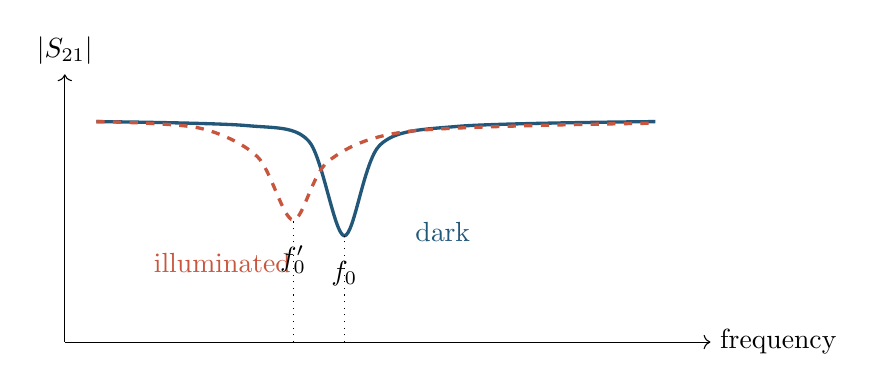
\begin{tikzpicture}[x=1cm,y=1cm]
\draw[->] (0,0)--(8.2,0) node[right]{frequency};
\draw[->] (0,0)--(0,3.4) node[above]{$|S_{21}|$};
\draw[very thick,KidBlue] plot[smooth] coordinates {(0.4,2.8)(2.3,2.75)(3.1,2.55)(3.55,1.35)(4.0,2.5)(5.0,2.74)(7.5,2.8)};
\draw[very thick,KidRed,dashed] plot[smooth] coordinates {(0.4,2.8)(1.7,2.72)(2.45,2.35)(2.9,1.55)(3.35,2.3)(4.4,2.68)(7.5,2.78)};
\node[KidBlue] at (4.8,1.4) {dark};
\node[KidRed] at (2.0,1.0) {illuminated};
\draw[dotted] (3.55,0)--(3.55,1.35) node[below,yshift=-2mm]{$f_0$};
\draw[dotted] (2.9,0)--(2.9,1.55) node[below,yshift=-2mm]{$f_0'$};
\end{tikzpicture}
\end{center}

\subsection{真正观测时：通常固定 probe tone，不需要不停扫频}
实际读出往往选取 $f_{\rm probe}\approx f_0$，持续测量一个复数：
\[
\boxed{S_{21}(t)=I(t)+jQ(t).}
\]
当谐振器因光照发生轻微移动时，固定 probe tone 在 resonance 曲线上的相对位置发生变化，因此 $I$ 和 $Q$ 随时间变化。

\begin{center}
\begin{tikzpicture}[scale=1.05]
\draw[->] (-2.6,0)--(2.8,0) node[right]{$I$};
\draw[->] (0,-2.3)--(0,2.5) node[above]{$Q$};
\draw[very thick,KidBlue] (0.35,0.05) circle (1.55);
\fill[KidBlue] (1.05,1.42) circle (2pt) node[above right]{dark operating point};
\fill[KidRed] (0.72,1.55) circle (2pt) node[above left]{illuminated};
\draw[-{Latex[length=2mm]},very thick,KidRed] (1.05,1.42)--(0.72,1.55);
\node[align=center] at (-1.4,-1.55) {扫频时形成\\近似 IQ 圆};
\end{tikzpicture}
\end{center}

这一步把 KID 与熟悉的数字接收机世界连接起来：最终进入 ADC/DSP 的不是“光子”本身，而是经过谐振器转导后的复基带响应。

\section{为什么读出微波不会自己把 Cooper pair 大量打碎？}
KID 中通常同时存在两种频率尺度：
\begin{align*}
\nu_{\rm signal} &\sim \text{几十到数百 GHz（毫米/亚毫米波）},\\
\nu_{\rm readout} &\sim \text{几百 MHz 到数 GHz（微波）}.
\end{align*}
设计上常希望
\[
h\nu_{\rm readout}<2\Delta,
\]
使单个 readout photon 的能量低于直接 pair-breaking threshold；与此同时
\[
h\nu_{\rm signal}>2\Delta,
\]
使目标光子能够被探测。

\begin{mistakebox}
“读出微波完全不影响超导态”也过于绝对。虽然单个低频 readout photon 通常不能直接 pair break，但过高读出功率仍会引起谐振器非线性、加热、准粒子分布变化等效应。因此实际系统存在最佳 readout power，而不是越大越好。
\end{mistakebox}

\section{LEKID 为什么尤其漂亮：同一块 meander 做两份工作}

\begin{center}
\begin{tikzpicture}[node distance=10mm and 13mm]
\node[flowbox,fill=KidGold!18,minimum width=31mm] (rad) {\SI{150}{GHz}\\入射辐射};
\node[flowbox,fill=KidTeal!10,right=of rad,minimum width=42mm,minimum height=16mm] (mea) {meander inductor\\毫米波 absorber\\GHz kinetic inductor};
\node[flowbox,fill=KidBlue!8,right=18mm of mea,minimum width=31mm,minimum height=16mm] (idc) {IDC\\capacitor};
\draw[goldarrow] (rad.east)--node[above,font=\scriptsize]{光学吸收} (mea.west);
\draw[structlink] (mea.east)--(idc.west);
\node[draw=KidBlue!45,rounded corners=3mm,inner sep=4mm,fit=(mea)(idc),label={[font=\scriptsize,text=KidBlue]above:同一个 GHz LC resonator}] (resgroup) {};

\node[flowbox,fill=KidGray,below=17mm of idc,minimum width=34mm] (cpl) {耦合结构\\$Q_c$};
\node[flowbox,fill=KidGray,left=of cpl,minimum width=42mm] (feed) {feedline\\GHz probe $\rightarrow$ output};
\draw[structlink,dashed] (cpl.north)--node[right,font=\scriptsize]{互易耦合} (resgroup.south east);
\draw[structlink] (feed.east)--(cpl.west);
\end{tikzpicture}
\end{center}

在 LEKID 中，lumped inductor 的 meander 往往同时承担：
\begin{enumerate}
  \item \textbf{毫米波/亚毫米波 absorber}：入射场在图形化薄膜中驱动高频电流并沉积能量；
  \item \textbf{GHz resonator 的电感}：其 $L_g+L_k$ 与 IDC 共同决定微波共振。
\end{enumerate}
因此，毫米波光学设计和 GHz 谐振器设计并不是两个独立问题；它们通过同一块超导薄膜耦合在一起。

\begin{projectbox}
对于双偏振直接吸收 LEKID，分析一个几何结构时可以先问两个问题：\\
\textbf{光学问题：}它如何改变 \SI{150}{GHz} 场、电流分布、吸收和偏振选择性？\\
\textbf{读出问题：}它如何改变 $L_g$、$L_k$、$C$、$f_0$、$Q_i$、$Q_c$ 和可读出性？\\
这两个视角同时成立，才算真正理解 LEKID 几何设计。
\end{projectbox}

\section{把全章压缩成一张“因果链地图”}

\begin{center}
\begin{tikzpicture}[node distance=6mm and 13mm]
\node[flowbox,fill=KidGold!18,minimum width=58mm] (a) {$h\nu>2\Delta$\\信号功率被超导薄膜吸收};
\node[flowbox,below=of a,minimum width=58mm] (b) {Cooper pairs 被激发/破坏\\$N_{\qp}\uparrow$};
\node[flowbox,below=of b,minimum width=58mm] (c) {复电导与表面阻抗改变\\$\sigma_1,\sigma_2$ 改变};
\node[flowbox,fill=KidTeal!8,below left=8mm and 7mm of c,minimum width=45mm] (d1) {感性支路\\$L_k\uparrow$};
\node[flowbox,fill=KidTeal!8,below right=8mm and 7mm of c,minimum width=45mm] (d2) {耗散支路\\loss$\uparrow$, $Q_i\downarrow$};
\node[flowbox,fill=KidBlue!7,below=22mm of c,minimum width=66mm] (e) {谐振器响应改变\\$f_0$ 移动，notch 宽度/深度改变};
\node[flowbox,fill=KidBlue!7,below=of e,minimum width=66mm] (f) {固定 GHz probe tone\\所见 $S_{21}(t)$ 改变};
\node[flowbox,fill=KidGray,below=of f,minimum width=66mm] (g) {$I(t),Q(t)$\\数字后端估计光学信号};
\draw[flowarrow] (a.south)--(b.north);
\draw[flowarrow] (b.south)--(c.north);
\draw[flowarrow] (c.south west) to[out=-90,in=90] (d1.north);
\draw[flowarrow] (c.south east) to[out=-90,in=90] (d2.north);
\draw[flowarrow] (d1.south) to[out=-90,in=155] (e.north west);
\draw[flowarrow] (d2.south) to[out=-90,in=25] (e.north east);
\draw[flowarrow] (e.south)--(f.north);
\draw[flowarrow] (f.south)--(g.north);
\end{tikzpicture}
\end{center}

\section{本章的“公式阶梯”}
第一遍学习只需要按下面顺序记忆，不需要同时掌握所有微观细节。

\begin{enumerate}
  \item 光子能量：
  \[
  E_\gamma=h\nu.
  \]
  \item Pair-breaking threshold：
  \[
  h\nu\ge2\Delta,
  \qquad
  \Delta(0)\approx1.764k_BT_c.
  \]
  \item 动能电感的核心比例关系：
  \[
  L_k\propto\frac1{n_s}.
  \]
  \item LC resonance：
  \[
  f_0=\frac1{2\pi\sqrt{LC}},\qquad L=L_g+L_k.
  \]
  \item 小信号频移：
  \[
  \frac{\delta f_0}{f_0}=-\frac{\alpha}{2}\frac{\delta L_k}{L_k}.
  \]
  \item 品质因数关系：
  \[
  \frac1{Q_r}=\frac1{Q_i}+\frac1{Q_c}.
  \]
  \item 实验读出量：
  \[
  S_{21}=I+jQ.
  \]
\end{enumerate}

\section{六个最容易形成的错误直觉}
\begin{enumerate}
  \item \textbf{“KID 直接测光子的电信号。”}\\
  不对。光先改变超导材料，再改变谐振器，最后才改变微波传输。
  \item \textbf{“只要 $h\nu>\Delta$ 就可以 pair break。”}\\
  基本阈值应是 $2\Delta$。
  \item \textbf{“Kinetic inductance 就是导线弯弯曲曲形成的电感。”}\\
  不对。弯曲几何主要影响 $L_g$；$L_k$ 来自超导载流子的惯性。
  \item \textbf{“光照只是让 resonance 左移。”}\\
  不完整。它通常也改变损耗和 $Q_i$。
  \item \textbf{“KID 工作时必须持续扫频。”}\\
  通常扫频用于定位与标定，真正时间序列读出常使用固定 probe tones。
  \item \textbf{“读出功率越大，SNR 一定越好。”}\\
  不对。过强驱动会进入非线性、加热或改变准粒子状态。
\end{enumerate}

\section{Day 1 的 3--4 小时任务}
如果今天只围绕这一章学习，建议按以下顺序：

\noindent\begin{tabularx}{\textwidth}{p{1.8cm} X X}
\toprule
时间 & 任务 & 完成标准 \\
\midrule
35 min & 手画“光子 $\rightarrow$ IQ”因果链，并写出每一箭头为什么成立 & 不看讲义可口述完整链条 \\
45 min & 独立重算 Al 在 $T_c=\SI{1.2}{K}$ 时的 $\Delta$、$2\Delta$ 和 $\nu_{\rm pb}$；再算 \SI{150}{GHz} 光子能量 & 能判断某个频率是否满足 pair-breaking 条件 \\
55 min & 从 $f_0=1/(2\pi\sqrt{LC})$ 推导小信号 $\delta f_0/f_0$，理解 $\alpha$ 的意义 & 推导不用背结果 \\
60 min & Python 画 notch resonator 的 $|S_{21}|$ 与 IQ 圆；令 $f_0$ 左移并比较固定 probe tone 的 $\Delta I,\Delta Q$ & 得到至少 3 张图 \\
30 min & 阅读 Day et al. (2003) 的摘要与图 1，并回看本章因果链 & 能指出论文实验的“被测量量”在哪里 \\
20 min & 闭卷回答本章 8 道题 & 至少 6 题能完整解释“为什么” \\
\bottomrule
\end{tabularx}

\section{闭卷理解检查}
\begin{checkpointbox}
不查资料，尝试回答：
\begin{enumerate}
  \item 为什么 pair-breaking threshold 是 $2\Delta$？
  \item 为什么 \SI{150}{GHz} 对 Al 是一个合理的 pair-breaking 频率，而 \SI{5}{GHz} 通常不是？
  \item $N_{\qp}$ 增加后，为什么不能只讨论 $L_k$ 而忽略 $Q_i$？
  \item $L_g$ 与 $L_k$ 的能量分别储存在什么地方？
  \item 为什么 $L_k$ 增加通常导致 $f_0$ 降低？
  \item 什么是 $Q_i,Q_c,Q_r$？
  \item 为什么实际观测可以固定 probe tone，而不必一直扫频？
  \item 用一句完整的话解释：LEKID 的 meander 为什么同时是 absorber 和 resonator inductor？
\end{enumerate}
\end{checkpointbox}

\section{本章结束后你应该拥有的“一个句子”}
如果只能保留一句话，应当是：

\begin{formula}
\centering
\Large
\textbf{KID 用高于能隙阈值的光改变超导薄膜的准粒子与复电导，再用高 $Q$ 微波谐振器把这种微小变化转成可精确测量的 $S_{21}=I+jQ$ 变化。}
\end{formula}


\part{超导材料与微波谐振器}
\chapter{动能电感：为什么“载流子的惯性”会变成一个可测的电感？}
\chapterguide
{KID 名字里的“kinetic inductance”不是修辞；如果不理解它，就无法解释光为什么会推动谐振频率变化。}
{电流、电场、$V=L\,dI/dt$ 和最基本的 LC 谐振直觉。}
{从载流子运动方程和能量两条路线推出 $L_k$；解释 $n_s$、几何尺寸、$L_{k,\Box}$ 与动能电感分数 $\alpha$。}
{超流载流子的惯性提供了一种可以被光间接调制的电感。}

\begin{goalbox}
这一章只解决一个核心问题：\textbf{为什么超导载流子的运动惯性可以从器件端口看成一个电感 $L_k$？}
学完后你应能：
\begin{enumerate}
  \item 从 $m\,dv/dt=qE$ 独立推到一段均匀超导条带的 $L_k$；
  \item 用能量法再次得到同一个结果，并解释“电感储能”储在哪里；
  \item 理解 London penetration depth $\lambda_L$ 与 $L_k$ 的关系；
  \item 把三维电感化成薄膜工程中常用的 sheet kinetic inductance $L_{k,\Box}$；
  \item 判断长度、线宽、膜厚、超流密度怎样改变 $L_k$，以及为什么 $\alpha$ 决定频率响应；
  \item 知道电磁仿真中把金属简单设成 PEC 时，哪一部分 KID 物理会被漏掉。
\end{enumerate}
\end{goalbox}

\begin{tcolorbox}[colback=KidBlue!4,colframe=KidBlue!60,boxrule=0.7pt,arc=2mm,title=先认清两套语言：这一章为什么突然出现 $E$、$J$、$n_s$ 和 $v$？,fonttitle=\bfseries]
前面一直在用\textbf{电路语言}：电压 $V$、电流 $I$、电感 $L$。这一章要回答“$L_k$ 从材料内部哪里来”，所以必须短暂切换到\textbf{材料语言}：电场 $E$、电流密度 $J$、有效超导载流子密度 $n_s$ 和平均速度 $v$。

两套语言并不矛盾。对一段近似均匀的条带，最重要的转换只有
\[
\boxed{V=El,\qquad I=JA.}
\]
其中 $l$ 是条带长度，$A=wt$ 是横截面积，而 $J$ 可以先直观理解成“\textbf{每单位横截面积流过多少电流}”。接下来的推导只是把微观的“载流子需要被加速”翻译成端口看到的 $V=L_k\,dI/dt$。

此处也\textbf{不要求已经理解 Cooper pair 的完整量子理论}。$m^*$、$q^*$、$n_s$ 先作为有效参数使用；第 4 章会再解释超导状态和准粒子到底是什么。
\end{tcolorbox}

\section{先把“电感”拆成两种储能机制}
对于 LEKID 的一段 meander，总电感可以写成
\[
L=L_g+L_k.
\]
这两个量从端口看都满足“电流变化越快，需要的电压越大”，但物理储能位置不同。

\begin{center}
\begin{tikzpicture}[node distance=10mm and 12mm]
\node[flowbox,fill=KidBlue!6,minimum width=46mm,minimum height=18mm] (c) {$C$：电容\\能量主要储存在电场\\$U_E=\tfrac12CV^2$};
\node[flowbox,fill=KidGold!13,right=of c,minimum width=46mm,minimum height=18mm] (lg) {$L_g$：几何电感\\能量主要储存在磁场\\$U_B=\tfrac12L_gI^2$};
\node[flowbox,fill=KidTeal!10,right=of lg,minimum width=46mm,minimum height=18mm] (lk) {$L_k$：动能电感\\能量储存在载流子动能\\$U_k=\tfrac12L_kI^2$};
\end{tikzpicture}
\end{center}

\begin{intuitionbox}
“meander 弯得很多，所以它有 kinetic inductance”是错误直觉。弯折、回流路径和周围磁场首先影响 $L_g$；$L_k$ 的根源是\textbf{有质量的超导载流子被交流电场加速}。即使一根完全笔直的超导条带，也有 $L_k$。
\end{intuitionbox}

\section{第一条推导：从载流子惯性到 $V=L_k\,dI/dt$}

\subsection{步骤 1：电场使超导载流子加速}
先使用一个故意简化但非常有用的模型。令有效超导载流子的质量、电荷和数密度分别为 $m^*$、$q^*$、$n_s$。忽略散射时，沿导线方向有
\[
m^*\frac{dv}{dt}=q^*E.
\]
电流密度为
\[
J=n_s q^* v.
\]
因此
\[
\frac{dJ}{dt}=n_s q^*\frac{dv}{dt}
=\frac{n_s(q^*)^2}{m^*}E,
\]
从而
\begin{formula}
\[
\boxed{
E=\frac{m^*}{n_s(q^*)^2}\frac{dJ}{dt}
}
\]
\end{formula}

这已经具有“感性”特征：电场不是与 $J$ 本身成正比，而是与 $dJ/dt$ 成正比。

\subsection{步骤 2：从电流密度变成器件端口的电流}
考虑一段长度为 $l$、宽度为 $w$、厚度为 $t$ 的均匀条带，截面积
\[
A=wt.
\]
若电流密度近似均匀，则
\[
J=\frac{I}{A},\qquad V=El.
\]
代入上式：
\[
V=\frac{m^*l}{n_s(q^*)^2A}\frac{dI}{dt}.
\]
与普通电感定义
\[
V=L\frac{dI}{dt}
\]
逐项比较，得到最基础的 kinetic inductance：
\begin{formula}
\[
\boxed{
L_k=\frac{m^*l}{n_s(q^*)^2A}
=\frac{m^*l}{n_s(q^*)^2wt}
}
\]
\end{formula}
\formulaexplain
{在这个均匀条带模型中，$L_k\propto l$，并与 $n_s$、$w$、$t$ 成反比；电荷以 $(q^*)^2$ 进入。}
{同样的总电流若被迫通过更少的超流载流子或更小的横截面，每个有效载流子需要更大的运动速度，因此储存更多集体动能；端口就看到更大的动能电感。}
{它提供非常有用的第一轮设计趋势：加长、变窄、变薄或降低有效 $n_s$ 都会提高 $L_k$。这能指导 meander 参数扫描，也解释为什么薄膜工艺偏差会推移 GHz resonance。}
{推导假设条带均匀、局域响应、忽略散射且电流密度近似均匀。真实薄膜还可能处于 dirty limit，弯角会有 current crowding，有限厚度与频率效应也会改变结果；精确设计应使用 $L_{k,\square}$、复电导/表面阻抗或全波模型。}

\subsection{关于 $2e$、$2m_e$ 与 $n_s$ 的一个重要约定}
有的教材把 $n_s$ 定义为 Cooper-pair density，此时自然使用 $q^*=2e$、$m^*\approx2m_e$；另一些教材把 $n_s$ 写成“参与超流的电子密度”，公式中则使用电子的 $e,m_e$。只要\textbf{密度定义与电荷/质量定义保持一致}，最终物理结果是一致的。初学阶段最危险的是把两套约定混用，从而凭空多出一个 2 或 4 的因子。

\section{第二条推导：用能量法检查结果}
如果前面的代数让你觉得 kinetic inductance 仍然只是“人为定义”，能量法会更直观。

体积 $Al$ 内的超导载流子总动能为
\[
U_k=\frac12(n_sAl)m^*v^2.
\]
又因为
\[
I=J A=n_sq^*vA,
\]
所以
\[
v=\frac{I}{n_sq^*A}.
\]
代回：
\[
U_k
=\frac12\frac{m^*l}{n_s(q^*)^2A}I^2.
\]
而任意等效电感的储能写作
\[
U_L=\frac12LI^2.
\]
因此再次得到
\[
\boxed{L_k=\frac{m^*l}{n_s(q^*)^2A}}.
\]

\begin{checkpointbox}
这两条推导其实在说同一件事：\textbf{建立电流需要让有质量的超导载流子获得速度，因此需要储存动能；而一个端口只要以 $\tfrac12LI^2$ 的形式储能，就会表现为电感。}
\end{checkpointbox}

\section{从公式直接读出四个工程结论}
把
\[
L_k=\frac{m^*l}{n_s(q^*)^2wt}
\]
盯着看，不做任何复杂理论，就已经可以得到：
\begin{enumerate}
  \item \textbf{条带越长，$L_k$ 越大：} $L_k\propto l$；
  \item \textbf{线越窄，$L_k$ 越大：} $L_k\propto1/w$；
  \item \textbf{膜越薄，$L_k$ 越大：} 在均匀电流近似下 $L_k\propto1/t$；
  \item \textbf{超流密度越小，$L_k$ 越大：} $L_k\propto1/n_s$。
\end{enumerate}
最后一条正是 KID 探测原理的核心接口：光照或升温使超导凝聚态被激发，$n_s$ 有效下降，于是 $L_k$ 上升。

\begin{center}
\begin{tikzpicture}[node distance=7mm and 10mm]
\node[flowbox,fill=KidGray,minimum width=32mm] (geom) {几何旋钮\\$l\uparrow,w\downarrow,t\downarrow$};
\node[flowbox,fill=KidGold!13,below=of geom,minimum width=32mm] (state) {材料/状态\\$n_s\downarrow$};
\node[flowbox,fill=KidTeal!10,right=17mm of $(geom)!0.5!(state)$,minimum width=31mm] (lk) {$L_k\uparrow$};
\node[flowbox,fill=KidBlue!7,right=7mm of lk,minimum width=36mm] (alpha) {$\alpha=\dfrac{L_k}{L_g+L_k}$\\通常增大};
\node[flowbox,fill=KidBlue!7,right=7mm of alpha,minimum width=35mm] (resp) {相同材料扰动\\产生更大 $|\delta f_0|$};
\draw[influence] (geom.east) to[bend left=12] (lk.north west);
\draw[influence] (state.east) to[bend right=12] (lk.south west);
\draw[flowarrow] (lk.east)--(alpha.west);
\draw[flowarrow] (alpha.east)--(resp.west);
\end{tikzpicture}
\end{center}

\begin{mistakebox}
“线越窄、膜越薄一定越好”同样不成立。它们虽然能提高 $L_k$ 和潜在 responsivity，却也会改变毫米波表面阻抗匹配、临界电流、非线性、工艺均匀性、损耗和 $Q_i$。KID 设计几乎总是在多目标约束下寻找平衡，而不是最大化单个参数。
\end{mistakebox}

\section{London penetration depth：把 $n_s$ 藏进一个可测的长度尺度}
London 理论把超流密度写进 penetration depth：
\[
\boxed{
\lambda_L^2=\frac{m^*}{\mu_0n_s(q^*)^2}
}
\]
于是前面的均匀电流公式立刻变成
\begin{formula}
\[
\boxed{
L_k=\mu_0\lambda_L^2\frac{l}{A}
=\mu_0\lambda_L^2\frac{l}{wt}
}
\]
\end{formula}
这让一个非常重要的物理事实变得直观：
\[
n_s\downarrow\quad\Longleftrightarrow\quad\lambda_L\uparrow\quad\Longleftrightarrow\quad L_k\uparrow.
\]

\subsection{为什么叫 penetration depth？}
在块体超导体里，微波/磁场并不会像在真空中那样任意深入，而是在表面附近一个特征深度内衰减。$\lambda_L$ 就是描述这种场穿透和超流屏蔽的长度尺度。后续进入复电导与表面阻抗时，我们会看到 $\lambda$、$\sigma_2$ 与 $L_k$ 实际上是同一感性物理的不同语言。

\section{薄膜最实用的语言：每方块动能电感 $L_{k,\Box}$}
对于 KID，我们经常面对几十纳米量级的长而窄薄膜条带。若膜足够薄，使厚度方向电流可以近似均匀，则
\[
L_k=\mu_0\lambda_L^2\frac{l}{wt}
=\left(\mu_0\frac{\lambda_L^2}{t}\right)\frac{l}{w}.
\]
定义
\begin{formula}
\[
\boxed{
L_{k,\Box}\equiv\mu_0\frac{\lambda_L^2}{t}
}
\qquad (t\ll\lambda_L\text{ 的简单 London 极限})
\]
\end{formula}
\formulaexplain
{$L_{k,\square}$ 把“材料 + 膜厚”的动能电感能力压缩成每一个几何方块的电感；总条带近似为 $L_k\approx L_{k,\square}(l/w)$。}
{对均匀薄膜而言，一个长宽相等的方块无论整体尺寸多大，$l/w=1$。因此“每方块”不是一块固定面积，而是一种特别适合二维薄膜版图的几何计数语言。}
{版图只需统计有效 squares，就能把 wafer 的材料参数快速映射到 meander 的 $L_k$，非常适合早期手算、参数化几何和加工后模型更新。}
{这里写出的 $\mu_0\lambda_L^2/t$ 是 $t\ll\lambda_L$ 的简单局域 London 极限。实际 KID 常需考虑 dirty limit、有限温度与有限频率；工程上更可靠的 $L_{k,\square}$ 往往来自 $R_{\square,n}$ + $T_c$ 估算或低温谐振测量反演。}
以及方块数
\[
N_\Box=\frac{l}{w},
\]
就有
\[
\boxed{L_k\approx L_{k,\Box}N_\Box.}
\]

\begin{center}
\begin{tikzpicture}[x=1cm,y=1cm]
\fill[KidTeal!10] (0,0) rectangle (7.2,1.2);
\draw[KidDark!75,line width=0.8pt] (0,0) rectangle (7.2,1.2);
\foreach \x in {1.2,2.4,3.6,4.8,6.0}{\draw[KidDark!35] (\x,0)--(\x,1.2);}
\draw[flowarrow] (-0.8,0.6)--(-0.05,0.6) node[midway,above,font=\scriptsize]{$I$};
\draw[dimline] (0,-0.35)--(7.2,-0.35) node[midway,below,font=\scriptsize]{$l$};
\draw[dimline] (7.55,0)--(7.55,1.2) node[midway,right,font=\scriptsize]{$w$};
\node[font=\small] at (3.6,1.55) {$N_\Box=l/w$：宽度为 $w$ 的“方块”串联};
\end{tikzpicture}
\end{center}

“per square” 很适合平面器件：只要保持材料、膜厚和线宽定义一致，一个长条的总动能电感主要由方块数决定。对于真实 meander，弯角处的 current crowding、邻近导线磁耦合和非均匀电流会让简单 $N_\Box$ 估算产生偏差，因此它是\textbf{手算和设计直觉工具}，不是全波仿真的替代品。

\subsection{膜不再“很薄”时怎么办？}
局域 London 模型下，更一般的表面感性可写成
\[
L_{s}\approx\mu_0\lambda\,\coth\!\left(\frac{t}{\lambda}\right).
\]
当 $t\ll\lambda$ 时，$\coth(t/\lambda)\approx\lambda/t$，便退化到
\[
L_s\approx\mu_0\frac{\lambda^2}{t}.
\]
这里先把它作为“薄膜公式有适用范围”的提醒。真实 KID 薄膜还会受 dirty limit、温度和频率影响；这些会在 Mattis--Bardeen 章节统一处理。

\section{一个数值例子：为什么“每方块几 pH”最后也能变得重要？}
这里故意选一组\textbf{示意参数}，不是在宣称某种特定 Al 薄膜的真实材料常数：
\[
\lambda_{\rm eff}=\SI{200}{nm},\qquad t=\SI{20}{nm}.
\]
则薄膜近似给出
\[
L_{k,\Box}
=\mu_0\frac{\lambda_{\rm eff}^2}{t}
\approx \SI{2.5}{pH}\,/\Box.
\]
如果一段 meander 有约 $1000$ squares，那么仅动能电感就达到
\[
L_k\sim\SI{2.5}{nH}.
\]
这个量级已经足以显著参与 GHz 谐振器总电感。真正器件中必须使用实际薄膜测得或拟合的材料参数（如 $T_c$、$R_\Box$、$\Delta$、$\lambda$）或表面阻抗；不能把这个示意数值直接代入设计。

\section{从 $L_k$ 到 $\alpha$：为什么 KID 要关心“电感里有多少是动能的”}
重新定义
\[
\boxed{
\alpha=\frac{L_k}{L_g+L_k}.
}
\]
若光学扰动主要让 $L_k$ 发生微小变化，而 $L_g$ 和 $C$ 在一阶近似下不变，则
\[
\frac{\delta f_0}{f_0}
=-\frac12\frac{\delta L}{L}
=-\frac12\frac{\delta L_k}{L_g+L_k}.
\]
乘除一个 $L_k$：
\begin{formula}
\[
\boxed{
\frac{\delta f_0}{f_0}
=-\frac{\alpha}{2}\frac{\delta L_k}{L_k}.
}
\]
\end{formula}
所以 $\alpha$ 可以理解为“材料状态变化能够进入总谐振器电感的权重”。如果 $L_g\gg L_k$，材料发生同样的相对变化，却会被大量不敏感的几何电感稀释。

\begin{checkpointbox}
设两颗谐振器的 $\delta L_k/L_k$ 完全相同：A 的 $\alpha=0.05$，B 的 $\alpha=0.5$。在忽略其他差异时，B 的相对频移约为 A 的 10 倍。这并不证明 B 的总 NEP 一定更好，但说明它的\textbf{频率转导增益}更强。
\end{checkpointbox}

\section{对 LEKID 几何设计意味着什么？}
\begin{projectbox}
对于 \SI{150}{GHz} 双偏振直接吸收 LEKID，meander 的线宽、总路径长度和膜厚至少同时参与四件事：
\begin{enumerate}
  \item 决定毫米波表面电流分布和吸收匹配；
  \item 改变几何电感 $L_g$；
  \item 通过 $N_\Box$ 与薄膜参数改变 kinetic inductance $L_k$；
  \item 改变 $\alpha$，进而改变相同超导态扰动造成的 $\delta f_0/f_0$。
\end{enumerate}
所以“把 meander 线做细一点”不是单纯的 GHz 谐振频率调参，也不是单纯的毫米波吸收调参，而是在同时改动两个频率域。
\end{projectbox}

\section{一个与 Sonnet/CST 直接相关的提醒：PEC 会漏掉什么？}
如果在电磁仿真里把超导薄膜完全当作 perfect electric conductor（PEC），求解器仍然可以计算：
\begin{itemize}
  \item 几何电容和大部分 $L_g$；
  \item 电流路径、耦合、辐射和很多几何效应；
  \item 在相应模型下的毫米波场分布。
\end{itemize}
但一个理想 PEC 本身没有“载流子惯性对应的表面感抗”，因此不会自动给出真实的 superconducting $L_k$ 和相关耗散。若目标是预测真实 GHz resonance frequency、材料引起的频移或 $Q_i$，通常需要把实际超导薄膜的 sheet inductance / surface impedance / 合适的超导材料模型带入。

\begin{center}
\begin{tikzpicture}[node distance=8mm and 13mm]
\node[flowbox,fill=KidGray,minimum width=40mm] (geo) {几何模型\\meander / IDC / feedline};
\node[flowbox,fill=KidRed!5,below left=12mm and 4mm of geo,minimum width=43mm] (pec) {若金属设为 PEC\\主要得到 $L_g,C$ 与几何耦合};
\node[flowbox,fill=KidTeal!8,below right=12mm and 4mm of geo,minimum width=46mm] (sup) {若加入超导表面阻抗\\可包含 $L_k$ 与材料耗散};
\node[flowbox,fill=KidBlue!7,below=27mm of geo,minimum width=58mm] (pred) {与实测 $f_0,Q_i$ 比较\\判断几何误差还是材料模型误差};
\draw[flowarrow] (geo.south west) to[out=-90,in=90] (pec.north);
\draw[flowarrow] (geo.south east) to[out=-90,in=90] (sup.north);
\draw[flowarrow] (pec.south) to[out=-90,in=155] (pred.north west);
\draw[flowarrow] (sup.south) to[out=-90,in=25] (pred.north east);
\end{tikzpicture}
\end{center}

这也是为什么以后做“仿真--实测闭环”时，不能看到 resonance 对不上就立即把问题归咎于几何。\textbf{几何电感、电容、动能电感、材料损耗和工艺偏差都可能把 $f_0$ 推动。}

\section{这一章暂时没有做什么}
为了不把第一轮学习变成公式堆积，本章刻意没有完整推导：
\begin{itemize}
  \item BCS 中 $n_s(T)$ 与 $N_{qp}(T)$ 的严格关系；
  \item dirty-limit 超导薄膜的 $L_{k,\Box}\approx\hbar R_\Box/(\pi\Delta)$ 等常用结果；
  \item 复电导 $\sigma_1-i\sigma_2$ 与 surface impedance 的严格关系；
  \item Mattis--Bardeen 积分和有限频率、有限温度修正。
\end{itemize}
这些不是被忽略，而是被放到下一层理论中。现在先确保 $L_k$ 的物理来源已经不再神秘。

\section{本章的公式阶梯}
\begin{enumerate}
  \item 载流子动力学：
  \[
  m^*\frac{dv}{dt}=q^*E.
  \]
  \item 电流密度：
  \[
  J=n_sq^*v.
  \]
  \item 均匀条带的动能电感：
  \[
  \boxed{L_k=\frac{m^*l}{n_s(q^*)^2wt}}.
  \]
  \item London penetration depth：
  \[
  \boxed{\lambda_L^2=\frac{m^*}{\mu_0n_s(q^*)^2}}.
  \]
  \item 薄膜每方块动能电感：
  \[
  \boxed{L_{k,\Box}\approx\mu_0\frac{\lambda_L^2}{t}}.
  \]
  \item 总动能电感：
  \[
  L_k\approx L_{k,\Box}\frac{l}{w}.
  \]
  \item 动能电感占比与小信号频移：
  \[
  \boxed{\alpha=\frac{L_k}{L_g+L_k}},\qquad
  \boxed{\frac{\delta f_0}{f_0}=-\frac{\alpha}{2}\frac{\delta L_k}{L_k}}.
  \]
\end{enumerate}

\section{建议用 60--90 分钟完成的手算与代码任务}
\begin{enumerate}
  \item 不看讲义，从 $m\,dv/dt=qE$ 推到 $L_k=m^*l/[n_s(q^*)^2wt]$；
  \item 再用 $U_k=\tfrac12nmv^2V$ 独立推一次，检查两条路线是否一致；
  \item 写 10 行左右 Python：令 $L_g=8\,\mathrm{nH}$、$L_k$ 从 $0.5$ 到 $8\,\mathrm{nH}$ 扫描，画出 $\alpha$ 和 $f_0$ 的变化；
  \item 再令 $\delta L_k/L_k=10^{-4}$，画 $\alpha$ 从 0 到 1 时 $|\delta f_0/f_0|$ 的变化；
  \item 最后用一句话回答：\textbf{为什么 KID 不是“几何电感探测器”？}
\end{enumerate}

\section{闭卷理解检查}
\begin{checkpointbox}
\begin{enumerate}
  \item 一根完全笔直的超导条带有没有 kinetic inductance？为什么？
  \item $L_g$ 与 $L_k$ 分别把能量储存在哪里？
  \item 为什么 $L_k\propto1/n_s$？
  \item 把线宽减半，在最简单均匀电流模型里 $L_k$ 如何变化？
  \item 什么叫“每方块电感”？为什么 $l/w$ 没有量纲？
  \item 为什么 PEC 仿真可以给出漂亮的 resonance，却仍可能把真实 $f_0$ 算偏？
  \item $\alpha$ 大意味着什么？它为什么不是“越大越好”的单一优化目标？
\end{enumerate}
\end{checkpointbox}


\chapter{超导基础最小知识集：Cooper pair、能隙与准粒子}
\chapterguide
{前面已经知道“光会让 $L_k$ 变化”，这一章负责打开材料内部的黑箱：光到底改变了什么微观状态。}
{第 2--3 章的主因果链；不要求先修完整 BCS 理论。}
{解释 Cooper pair、能隙 $\Delta$、准粒子、pair breaking、热准粒子和准粒子寿命，并判断给定光子能否破对。}
{KID 关心的超导基础，是“能量怎样改变准粒子人口，以及这种改变能维持多久”。}

\begin{goalbox}
这一章不试图把 BCS 理论从头推完。目标是建立一套足够支撑 KID 设计的“最小超导语言”。学完后，你应该能回答：
\begin{enumerate}
  \item 普通金属与超导态在“可激发的低能状态”上有什么本质区别？
  \item Cooper pair 为什么不能简单理解成两个紧紧抱在一起的电子？
  \item 能隙 $\Delta$、临界温度 $T_c$ 与 pair-breaking 阈值之间是什么关系？
  \item 什么是 quasiparticle（准粒子），为什么 KID 真正关心的是 $N_{\qp}$？
  \item 为什么热准粒子在低温下呈指数压低，而真实器件仍可能存在 excess quasiparticles？
  \item pair breaking、recombination（复合）与 quasiparticle lifetime（准粒子寿命）如何决定 KID 的响应速度与灵敏度？
\end{enumerate}
\end{goalbox}

\section{为什么现在才补“超导基础”？}
前两章我们已经知道：
\[
P_{\rm abs}\rightarrow N_{\qp}\rightarrow L_k,Q_i\rightarrow f_0,S_{21}.
\]
第 3 章又从载流子惯性推出了 $L_k$。但这里一直有一个“黑箱”：
\[
\boxed{\text{光子为什么会让 }N_{\qp}\text{ 增加？}\qquad
N_{\qp}\text{ 到底是什么？}}
\]

本章就是打开这个黑箱。对 KID 设计者来说，最重要的不是会写完整 BCS gap equation，而是建立下面这条微观链：
\[
\boxed{
T_c\rightarrow\Delta(T)
\rightarrow
\text{准粒子可激发能量}
\rightarrow
N_{\qp}(T,P_{\rm abs})
\rightarrow
\tau_{\qp}
\rightarrow
L_k,Q_i,S_{21}
}
\]

\begin{intuitionbox}
把超导体想成一个“低能激发被能隙挡住的电子系统”。KID 的工作，本质上是用毫米波/亚毫米波给这个系统制造少量准粒子，再用 GHz 谐振器非常灵敏地读出这些准粒子改变了多少复电导。
\end{intuitionbox}

\begin{tcolorbox}[colback=KidTeal!5,colframe=KidTeal!70!black,boxrule=0.7pt,arc=2mm,title=在看能带图之前，先把三个词翻成普通话,fonttitle=\bfseries]
\begin{itemize}
  \item \textbf{$E_F$（Fermi energy，费米能）：}这里主要把它当作描述“哪些电子态最容易参与低能变化”的参考能量。图上画一条 $E_F$，不表示材料内部真的有一堵能量墙。
  \item \textbf{$\Delta$（energy gap，能隙）：}它是\textbf{激发能量上的门槛}，不是材料内部裂开了一条空间缝隙。对最低能的单个 BCS 准粒子，其激发能量至少为 $\Delta$。
  \item \textbf{quasiparticle（准粒子）：}它是描述超导体系激发的一种有效语言，不应简单等同为“一颗恢复正常的普通电子”。KID 之所以关心它，是因为准粒子人口变化会改变薄膜的微波电磁响应。
\end{itemize}
先抓住这三句话，再看 $E=\sqrt{\xi^2+\Delta^2}$，公式就不再只是突然出现的一串符号。
\end{tcolorbox}

\section{正常金属与超导态：区别不只是“电阻变成零”}

\subsection{正常金属：费米面附近有大量低能激发}
在金属中，电子填充到 Fermi energy（费米能）$E_F$ 附近。只要提供很小的能量，就可以在 $E_F$ 附近制造电子--空穴激发。对交流电流来说，电子还会不断受到晶格、杂质和缺陷散射，因此产生耗散。

这时可以用一句非常粗略但有用的话概括：
\[
\boxed{\text{正常金属在 }E_F\text{ 附近“很容易被激发”。}}
\]

\subsection{超导态：形成具有共同相位的配对基态}
对于常规超导体，温度降到 $T_c$ 以下后，费米面附近的一部分电子通过有效吸引相互作用形成 Cooper pairs，并进入一个具有宏观相干相位的配对基态。

这里有两个需要立即纠正的直觉：
\begin{itemize}
  \item 超导不是因为“电子突然不与任何东西碰撞”；
  \item Cooper pair 也不是两个电子变成了一颗局域的小分子。
\end{itemize}

真正关键的是：\textbf{体系的低能激发谱发生了重构，并出现能隙 $\Delta$。}

\begin{center}
\begin{tikzpicture}[x=1.05cm,y=0.78cm]
  \draw[->,draw=KidDark!75] (-4.4,0)--(4.7,0) node[right,font=\small] {$\xi=\varepsilon-E_F$};
  \draw[->,draw=KidDark!75] (0,-0.2)--(0,3.4) node[above,font=\small] {准粒子激发能量 $E$};

  \draw[dashed,draw=KidDark!45,line width=0.8pt] (-3.6,3.0)--(0,0)--(3.6,3.0);
  \node[font=\scriptsize,anchor=west,text=KidDark!65] at (2.05,2.75) {正常态：$E=|\xi|$};

  \draw[draw=KidBlue,line width=1.35pt,domain=-3.5:3.5,samples=100,smooth,variable=\x]
    plot ({\x},{sqrt(\x*\x+0.75*0.75)});
  \node[font=\scriptsize,text=KidBlue,anchor=west] at (2.0,2.05) {超导态：$E=\sqrt{\xi^2+\Delta^2}$};

  \draw[KidRed,-{Stealth[length=2mm]},line width=1pt] (-0.55,0.04)--(-0.55,0.72);
  \draw[KidRed,dashed,line width=0.7pt] (-0.55,0.75)--(0,0.75);
  \node[font=\scriptsize,text=KidRed,anchor=east] at (-0.67,0.39) {$\Delta$};
  \fill[KidBlue] (0,0.75) circle (1.3pt);
  \node[font=\scriptsize,text=KidDark!70] at (0,-0.42) {$E_F$};
\end{tikzpicture}
\end{center}

上图只想表达一件事：当 $\xi=0$，正常态可以有趋近于零的激发能量；而超导态的准粒子最小激发能量是 $\Delta$。

\section{Cooper pair：KID 需要掌握到什么程度？}

\subsection{一对典型的量子数}
在最简单的常规 $s$ 波 BCS 图景中，常把一对电子写成：
\[
(\mathbf{k},\uparrow),\qquad(-\mathbf{k},\downarrow).
\]
也就是近似相反动量、相反自旋的配对。晶格振动（phonon，声子）介导的有效吸引可以战胜一部分库仑排斥，使费米面附近的电子产生配对不稳定性。

\subsection{它不是“两颗电子抱成一个小球”}
Cooper pair 的空间尺度可以远大于晶格常数，许多 pair 彼此高度重叠。真正形成超导的是一个集体的配对凝聚态，而不是大量彼此独立的小分子。

因此我们以后写“打碎一个 Cooper pair”时，应该把它理解成：
\[
\boxed{\text{从配对基态中制造两个准粒子激发}}
\]
而不是机械地想象“把一根两电子化学键掰断”。

\begin{mistakebox}
“Cooper pair 的结合能就是 $2\Delta$”是容易误导的说法。对 KID 而言，最安全的表述是：\textbf{制造两个最低能准粒子激发至少需要约 $2\Delta$ 的能量}。$\Delta$ 是单个准粒子激发谱的能隙参数。
\end{mistakebox}

\section{BCS 能隙 $\Delta$：把材料与探测频率连接起来}

\subsection{零温弱耦合关系}
对于常规弱耦合 BCS 超导体，
\[
\boxed{\Delta_0\equiv\Delta(T=0)\approx1.764\,k_B T_c.}
\]
% STEP4B:gap-tc
\formulaexplain
{在弱耦合 BCS 极限，零温能隙 $\Delta_0$ 与临界温度 $T_c$ 成正比；比例系数约为 $1.764k_B$。}
{$T_c$ 和 $\Delta$ 都来自同一个配对能量尺度：升到 $T_c$ 附近时配对有序态消失，能隙也随之闭合。}
{只要先测到薄膜的 $T_c$，就能得到 $\Delta_0$ 的第一轮估计，并进一步估算 pair-breaking threshold $2\Delta_0/h$。这是材料筛选与 science band 匹配最便宜的一步。}
{$1.764$ 不是所有超导薄膜的普适常数。它对应常规、各向同性、弱耦合 $s$ 波 BCS 的零温极限；强耦合、非常规超导、薄膜无序和 proximity effect 都可能改变 $2\Delta_0/k_BT_c$。}


这条关系对 KID 特别重要，因为它把一个容易测量的材料参数 $T_c$ 直接变成能量尺度。

当 $T\rightarrow T_c$ 时，
\[
\Delta(T)\rightarrow0.
\]
工程计算中常用下面的近似插值来画趋势：
\[
\Delta(T)\approx
\Delta_0\tanh\!\left[
1.74\sqrt{\frac{T_c}{T}-1}
\right],\qquad 0<T<T_c.
\]
它是方便的 BCS-like 插值，不应被当成完整 gap equation 本身。

\subsection{pair-breaking 阈值}
要制造两个最低能准粒子，最基本阈值是：
\[
\boxed{h\nu_{\rm pb}\approx2\Delta.}
\]
在低温、弱耦合近似下：
\[
\boxed{
\nu_{\rm pb}(0)
\approx
\frac{2\Delta_0}{h}
\approx
73.5\ \mathrm{GHz/K}\times T_c.
}
\]

于是 KID 的材料选择第一次和观测频率直接相遇。

\begin{center}
\renewcommand{\arraystretch}{1.2}
\begin{tabular}{lcccc}
\toprule
材料 & 代表性 $T_c$ (K) & $\Delta_0$ (meV) & $\nu_{\rm pb}$ (GHz) & \SI{150}{GHz} 直接 pair break?\\
\midrule
Ti & 0.4 & 0.061 & 29 & 是 \\
Al & 1.2 & 0.182 & 88 & 是 \\
Nb & 9.2 & 1.40 & 676 & 否 \\
NbTiN & 14 & 2.13 & 1029 & 否 \\
\bottomrule
\end{tabular}
\end{center}

\noindent
上表只使用弱耦合公式与代表性 $T_c$ 做数量级估算。\textbf{真实薄膜的 $T_c$、能隙和强耦合修正会随材料配比、膜厚与沉积工艺改变。}

\begin{projectbox}
若吸收材料近似为 Al，$T_c\sim\SI{1.2}{K}$ 时 $\nu_{\rm pb}\sim\SI{88}{GHz}$，因此 \SI{150}{GHz} 光子高于 pair-breaking 阈值；而 1--5 GHz 读出微波远低于该阈值。这个频率层级正是 KID “高频光负责改变器件、低频微波负责询问器件”的材料基础。
\end{projectbox}

\section{准粒子：不是普通电子，而是超导体系的激发}

\subsection{最小能量}
BCS 准粒子能量写成：
\[
\boxed{
E_{\mathbf{k}}=\sqrt{\xi_{\mathbf{k}}^2+\Delta^2},
\qquad
\xi_{\mathbf{k}}=\varepsilon_{\mathbf{k}}-E_F.
}
\]
% STEP4B:qp-dispersion
\formulaexplain
{准粒子能量是 $\xi_{\mathbf{k}}$ 与 $\Delta$ 的平方和开根号，因此无论 $\xi$ 多接近零，都有 $E_{\mathbf{k}}\ge\Delta$。}
{超导转变不是把正常态能带简单平移，而是在费米面附近重构低能激发谱并打开能隙。准粒子因此是配对体系的激发，而不是一颗普通电子被单独“抬高”了能量。}
{这条色散关系解释了为什么热准粒子会被指数压低，也解释了 BCS density of states 和 Mattis--Bardeen 积分为什么在 $E\simeq\Delta$ 附近特别敏感。}
{这里使用理想、各向同性 $s$ 波 BCS 色散。真实薄膜中的 Dynes broadening、无序、proximity effect、非平衡分布或非常规配对会让理想能隙边缘被展宽或改变。}

因此：
\[
E_{\mathbf{k}}\ge\Delta.
\]

更严格地说，Bogoliubov quasiparticle 是电子与空穴自由度的量子叠加。KID 初学阶段暂时不需要推 Bogoliubov transformation，但要避免把 quasiparticle 简化成“一个从 Cooper pair 里掉出来的普通电子”。

\subsection{超导态密度状态}
理想 BCS $s$ 波超导体的归一化态密度可写成：
\[
\frac{N_s(E)}{N_0}
=
\begin{cases}
0, & |E|<\Delta,\\[0.4em]
\dfrac{|E|}{\sqrt{E^2-\Delta^2}}, & |E|>\Delta.
\end{cases}
\]

因此能隙内部没有理想单粒子激发态，并在 $|E|=\Delta$ 附近出现 coherence peak（相干峰）。这也是后面 Mattis--Bardeen 积分为什么总围着 $\Delta$ 附近的状态打转的根源。

\section{热准粒子：为什么降温如此有效？}

\subsection{Fermi--Dirac 占据}
准粒子的热占据服从：
\[
f(E,T)=\frac{1}{\exp(E/k_BT)+1}.
\]

当 $k_BT\ll\Delta$，热激发必须跨过能隙，因此平衡热准粒子密度近似为：
\[
\boxed{
n_{\qp}^{\rm th}(T)
\approx
2N_0\sqrt{2\pi k_BT\Delta}
\exp\!\left(-\frac{\Delta}{k_BT}\right)
}
\]
% STEP4B:thermal-qp
\formulaexplain
{热平衡准粒子密度由一个缓慢变化的平方根前因子乘上 $\exp[-\Delta/(k_BT)]$；深低温时真正支配数量级的是指数项。}
{制造热准粒子必须付出跨越能隙的能量。当 $k_BT\ll\Delta$ 时，热浴中具备这份能量的涨落极少，因此准粒子人口被指数压低。}
{它把制冷指标从“多少 mK”改写成更有意义的 $T/T_c$ 或 $\Delta/k_BT$。可用它估算理想 dark quasiparticle baseline，并判断继续降温是否仍可能带来显著收益。}
{公式假设热平衡、理想 BCS 态密度且处于低温近似，并依赖 $N_0$ 的明确定义。真实 KID 往往存在 excess/non-equilibrium quasiparticles；此时继续降低 bath temperature 也可能看不到公式预测的指数下降。}

其中 $N_0$ 是 normal-state Fermi level 处的 single-spin density of states（单自旋态密度）。

这个公式最重要的不是前面的平方根，而是：
\[
\boxed{n_{\qp}^{\rm th}\propto e^{-\Delta/k_BT}.}
\]

\subsection{把指数压低看成数量级}
令 $\Delta\approx\Delta_0=1.764k_BT_c$，则：
\[
\frac{n_{\qp}^{\rm th}}{2N_0\Delta_0}
\approx
\sqrt{\frac{2\pi(T/T_c)}{1.764}}
\exp\!\left(-\frac{1.764}{T/T_c}\right).
\]

\begin{center}
\begin{tabular}{ccc}
\toprule
$T/T_c$ & $n_{\qp}^{\rm th}/(2N_0\Delta_0)$ & 直觉 \\
\midrule
0.10 & $1.3\times10^{-8}$ & 极强指数压低 \\
0.20 & $1.25\times10^{-4}$ & 已高出约 $10^4$ 倍 \\
0.30 & $2.9\times10^{-3}$ & 热准粒子开始更难忽略 \\
0.50 & $3.9\times10^{-2}$ & 已远离“深低温”极限 \\
\bottomrule
\end{tabular}
\end{center}

\begin{intuitionbox}
对 KID 而言，“低温”最好不要只写成多少 mK，而要同时问 \textbf{$T/T_c$ 是多少}。同样 \SI{100}{mK}，对 $T_c=\SI{1.2}{K}$ 的 Al 和 $T_c=\SI{0.4}{K}$ 的 Ti 意义完全不同。
\end{intuitionbox}

\subsection{真实器件为什么常常比这个公式“脏”？}
理想热平衡公式给的是 baseline（基线），但真实 KID 在很低温时常出现 excess quasiparticles（额外准粒子），来源可能包括：
\begin{itemize}
  \item 外界毫米波、红外或黑体泄漏；
  \item 宇宙线、高能粒子或基底声子；
  \item 读出功率引起的加热与非平衡分布；
  \item 材料缺陷、陷阱和复杂的声子动力学。
\end{itemize}

因此：
\[
T\rightarrow0
\]
并不自动保证
\[
N_{\qp}\rightarrow0
\]
在真实系统里严格成立。实验上看到低温频移或损耗“饱和”，不能简单归因于 BCS 热准粒子。

\section{光子如何制造非平衡准粒子：从 pair breaking 到能量级联}

吸收一个满足 $h\nu>2\Delta$ 的光子后，最初产生的激发通常高于能隙边缘，随后通过 electron--phonon interaction（电子--声子相互作用）向低能弛豫。产生的高能声子又可能继续打断其他 pair。

\begin{center}
\begin{tikzpicture}[node distance=10mm and 10mm]
  \node[flowbox,fill=KidGold!22,minimum width=25mm] (ph) {$h\nu>2\Delta$\\吸收光子};
  \node[flowbox,right=of ph,minimum width=29mm] (hq) {高能准粒子\\初始激发};
  \node[flowbox,right=of hq,minimum width=27mm] (phon) {高能声子\\弛豫产生};
  \node[flowbox,right=of phon,minimum width=31mm] (pool) {近能隙准粒子池\\$N_{\qp}\uparrow$};
  \draw[flowarrow] (ph.east)--(hq.west);
  \draw[flowarrow] (hq.east)--(phon.west);
  \draw[flowarrow] (phon.east)--(pool.west);

  \node[flowbox,below=13mm of pool,minimum width=29mm] (rec) {两个准粒子复合\\形成 Cooper pair};
  \node[flowbox,left=of rec,minimum width=29mm] (p2) {$\sim2\Delta$ 声子};
  \node[flowbox,left=of p2,minimum width=28mm,fill=KidGray] (esc) {逃逸到基底\\或降能};
  \draw[flowarrow] (pool.south)--(rec.north);
  \draw[flowarrow] (rec.west)--(p2.east);
  \draw[flowarrow] (p2.west)--(esc.east);
  \draw[flowarrow] (p2.north east) to[out=65,in=215]
    node[pos=0.52,right,font=\scriptsize]{再次 pair break} (pool.south west);
\end{tikzpicture}
\end{center}

这说明一个高能光子并不一定只对应“两个准粒子”。常用一个 pair-breaking efficiency $\eta_{\rm pb}$ 把吸收能量中最终进入低能准粒子系统的比例概括进去：
\[
N_{\qp}^{\rm excess}
\sim
\eta_{\rm pb}\frac{E_{\rm abs}}{\Delta}.
\]

对连续吸收功率，也常用能量守恒的数量级形式：
\[
\boxed{
G_{\rm opt}
\sim
\eta_{\rm pb}\frac{P_{\rm abs}}{\Delta}
}
\]
% STEP4B:optical-generation
\formulaexplain
{准粒子产生率的量级等于“每秒真正吸收的能量”除以“形成低能准粒子所需的能量尺度 $\Delta$”，再乘能量转化效率 $\eta_{\rm pb}$。}
{一个高能光子首先产生高能激发，随后经电子--声子级联把能量重新分配；只有一部分吸收能量最终留在可被 KID 读出的低能准粒子池中。}
{它是从 optical simulation/光学标定得到的 $P_{\rm abs}$ 走向 responsivity 模型的入口：先把吸收功率转成 quasiparticle generation，再结合寿命得到稳态 $N_{\qp}$。}
{这是能量守恒的数量级表达，不是精确的微观级联公式。$\eta_{\rm pb}$ 依赖光子能量、材料、膜厚、声子逃逸/陷获等；且这里必须使用吸收功率 $P_{\rm abs}$，不能直接拿入射到系统前端的功率代入。}

其中 $G_{\rm opt}$ 是准粒子 generation rate（产生率）。精确系数与非平衡能量级联、声子逃逸和材料有关。

\section{recombination：为什么准粒子不会一直积累？}

两个准粒子可以重新进入 Cooper-pair condensate，并释放约 $2\Delta$ 的声子能量。于是 KID 中持续存在：
\[
\boxed{\text{generation}\quad\leftrightarrow\quad\text{recombination}}
\]

一个用于建立直觉的最小 rate equation（速率方程）是：
\[
\boxed{
\frac{dN_{\qp}}{dt}
=
G-\mathcal{R}N_{\qp}^2.
}
\]
% STEP4B:gr-rate-equation
\formulaexplain
{$G$ 是源项，$\mathcal{R}N_{\qp}^2$ 是二次损失项；两者相等时得到稳态 $N_{\qp,\rm ss}\propto\sqrt{G}$。}
{两颗准粒子需要相遇才能复合回 Cooper-pair condensate，因此在最简均匀模型里复合事件率随准粒子人口的平方增长。人口越高，复合也越快，系统自然不会无限积累。}
{这个方程非常适合做第一版负载扫描、稳态估算和时域数值实验，也能直接解释为何 responsivity 与 optical loading 往往不是严格线性的。}
{这里把体积、材料常数和声子反馈压进一个有效 $\mathcal{R}$。真实器件可能需要 Rothwarf--Taylor 方程，并考虑 phonon trapping、traps、diffusion、空间非均匀和非平衡能量分布。}

这里把几何体积等因素都吸收到有效复合系数 $\mathcal{R}$ 里，因此它只是教学用简化模型。

稳态满足：
\[
G=\mathcal{R}N_{\qp,\rm ss}^2,
\]
因此：
\[
\boxed{
N_{\qp,\rm ss}
=
\sqrt{\frac{G}{\mathcal{R}}}.
}
\]

这已经给出一个非常重要的非线性直觉：
\[
G\uparrow
\Rightarrow
N_{\qp}\uparrow
\Rightarrow
\text{recombination rate}\propto N_{\qp}^2\uparrow.
\]
所以准粒子不会无限累积。

\begin{mistakebox}
真实超导薄膜中的 quasiparticle--phonon 动力学通常需要 Rothwarf--Taylor 方程或 Kaplan 等人的电子--声子寿命理论。上面的 $G-\mathcal{R}N^2$ 是为了看懂“为什么存在稳态”和“为什么复合随 $N_{\qp}$ 增快”，不是完整材料模型。
\end{mistakebox}

\section{准粒子寿命 $\tau_{\qp}$：把微观物理连接到探测器速度}

如果在稳态附近突然增加少量准粒子，常可用单指数近似描述其恢复：
\[
\boxed{
\delta N_{\qp}(t)
=
\delta N_{\qp}(0)e^{-t/\tau_{\qp}}.
}
\]
% STEP4B:qp-lifetime
\formulaexplain
{小扰动按 $e^{-t/\tau_{\qp}}$ 衰减；经过一个 $\tau_{\qp}$，扰动剩下初值的 $1/e$。$\tau_{\qp}$ 因而直接定义恢复速度。}
{这是把非线性的 generation--recombination 动力学在某个稳态附近线性化后的结果：足够小的扰动看到一个局部的一阶恢复率。}
{从光脉冲、heater pulse 或加载阶跃的时间序列拟合 $\tau_{\qp}$，可以估计 detector bandwidth，并与 resonator ring-down time 比较究竟哪一环更慢。}
{单指数只在小扰动且存在一个主导时间常数时成立。强脉冲、空间扩散、多个准粒子池、声子陷获或读出链滤波都可能产生多指数或非指数恢复。}


对前面的简化模型线性化：
\[
\frac{d\,\delta N_{\qp}}{dt}
\approx
-2\mathcal{R}N_{\qp,\rm ss}\,\delta N_{\qp},
\]
所以：
\[
\tau_{\qp}
\sim
\frac{1}{2\mathcal{R}N_{\qp,\rm ss}}.
\]

它告诉我们：
\begin{itemize}
  \item 准粒子越少，复合事件越难相遇，寿命可能更长；
  \item 光学负载升高后 $N_{\qp}$ 增大，实际有效寿命常会缩短；
  \item 声子若被薄膜/基底结构反复吸收，phonon trapping 会改变观测到的有效寿命。
\end{itemize}

如果系统只有一个主导一阶时间常数，则：
\[
f_{\rm 3dB}\sim\frac{1}{2\pi\tau_{\qp}}.
\]

但 KID 还有谐振器自己的 ring-down time（衰减时间）：
\[
\boxed{
\tau_{\rm res}
=
\frac{Q_r}{\pi f_0}.
}
\]
真实时域响应通常同时受到 $\tau_{\qp}$ 与 $\tau_{\rm res}$ 约束，较慢的一环往往更容易成为带宽瓶颈。

\begin{intuitionbox}
较长的 $\tau_{\qp}$ 往往意味着同样的持续光功率可以在器件中“积累”更多准粒子，从而有利于 responsivity；但它也让响应变慢。KID 的灵敏度与时间响应并不是两个完全独立的设计指标。
\end{intuitionbox}

\section{材料选择的一条核心轴：同时比较 $T/T_c$ 与 $h\nu/2\Delta$}

现在可以把材料选择压缩成两个无量纲问题：
\[
\boxed{
\frac{T}{T_c}\quad\text{有多小？}
}
\qquad
\boxed{
\frac{h\nu}{2\Delta}\quad\text{是否大于 1？}
}
\]

前者控制 thermal quasiparticle baseline 的数量级；后者决定入射光是否具备直接 pair breaking 的能量条件。

这会产生一个很真实的工程 trade-off：
\begin{itemize}
  \item 降低 $T_c$：降低 pair-breaking threshold，并往往提高 kinetic inductance sensitivity；
  \item 但在同样 bath temperature 下，$T/T_c$ 变大，热准粒子更难压低；
  \item 提高 $T_c$：有利于低损耗和热稳定，但可能让目标光子根本达不到 $2\Delta$。
\end{itemize}

因此“$T_c$ 越低越好”或“$T_c$ 越高越好”都不是普遍结论。

\section{映射到当前 \SI{150}{GHz} 双偏振 LEKID}

\begin{projectbox}
对当前 \SI{150}{GHz} LEKID，建议以后每次谈材料或仿真参数，都同时写出四个量：
\[
T_c,\qquad
\Delta_0,\qquad
\nu_{\rm pb}=\frac{2\Delta_0}{h},\qquad
T/T_c.
\]
这样可以在设计表格里一眼判断“目标光是否能 pair break”和“工作温度是否足够深低温”。

若使用 Al 类低能隙吸收膜：
\begin{itemize}
  \item \SI{150}{GHz} 通常高于 pair-breaking threshold；
  \item GHz readout tone 单个光子远低于 $2\Delta$，通常不会直接 pair break；
  \item 但过高 readout power 仍可能通过加热、非平衡分布、多光子过程或电流非线性改变准粒子系统，所以“低于 $2\Delta$”不等于“读出功率可以无限加大”。
\end{itemize}

若只使用 Nb/NbTiN 这类高 $T_c$ 材料作为吸收体，\SI{150}{GHz} 可能低于直接 pair-breaking threshold。工程上因此常见“高能隙材料负责低损耗微波结构、低能隙材料负责吸收/准粒子产生”的混合材料思路。
\end{projectbox}

\section{七个常见误区}

\begin{mistakebox}
\begin{enumerate}
  \item \textbf{“Cooper pair 就是两个电子形成的小分子。”}\\
  不对。BCS pair 是高度重叠的集体量子配对结构。
  \item \textbf{“超导无电阻是因为电子不再散射。”}\\
  过度简化。关键是配对凝聚态与有能隙的激发谱。
  \item \textbf{“$\Delta$ 就是打碎一对电子所需的全部能量。”}\\
  对 KID 最安全的说法是：单个最低能准粒子至少需要 $\Delta$，制造两个准粒子的 pair-breaking threshold 约为 $2\Delta$。
  \item \textbf{“只要 $h\nu>2\Delta$，吸收效率就一定很高。”}\\
  错。阈值只说明能量上允许 pair breaking；光学吸收还取决于 sheet impedance、几何、偏振、backshort 等。
  \item \textbf{“温度足够低后，$N_{\qp}$ 一定严格趋近零。”}\\
  理想热平衡模型如此，但真实器件可能被外界辐射、基底声子和读出功率维持在非平衡准粒子底噪上。
  \item \textbf{“读出频率低于 $2\Delta/h$，所以 readout power 与超导状态完全无关。”}\\
  错。单个读出光子不能直接 pair break，不代表强微波场不会产生加热和非线性。
  \item \textbf{“$T_c$ 越低，KID 一定越灵敏。”}\\
  不成立。还要同时考虑工作温度、热准粒子、薄膜损耗、可加工性、$\alpha$、噪声和光学匹配。
\end{enumerate}
\end{mistakebox}

\section{本章公式阶梯}

第一层，只记能隙：
\[
\boxed{\Delta_0\approx1.764k_BT_c}
\]

第二层，把能隙变成探测频率门槛：
\[
\boxed{h\nu_{\rm pb}\approx2\Delta}
\]

第三层，认识准粒子的激发谱：
\[
\boxed{E_{\mathbf{k}}=\sqrt{\xi_{\mathbf{k}}^2+\Delta^2}}
\]

第四层，看懂为什么冷却能压低 dark quasiparticles：
\[
\boxed{
n_{\qp}^{\rm th}
\approx
2N_0\sqrt{2\pi k_BT\Delta}
e^{-\Delta/k_BT}
}
\]

第五层，把光学负载写成 generation--recombination：
\[
\boxed{
\frac{dN_{\qp}}{dt}
=
G-\mathcal{R}N_{\qp}^2
}
\]

第六层，把准粒子动力学连接到响应速度：
\[
\boxed{
\delta N_{\qp}(t)\propto e^{-t/\tau_{\qp}}
}
\]

最后重新接回 KID：
\[
\boxed{
N_{\qp}
\rightarrow
\sigma_1,\sigma_2
\rightarrow
L_k,Q_i
\rightarrow
S_{21}
}
\]
下一章将正式打开中间这一步：Mattis--Bardeen 与 surface impedance。

\section{建议用 90--120 分钟完成的代码与手算任务}

\begin{enumerate}
  \item 写一个函数，用 $T_c$ 计算 $\Delta_0$ 与 $\nu_{\rm pb}$，分别代入 Ti、Al、Nb、NbTiN 的代表性 $T_c$；
  \item 画出
  \[
  \Delta(T)/\Delta_0
  \]
  对 $T/T_c$ 的 BCS-like 插值曲线；
  \item 用低温近似画
  \[
  n_{\qp}^{\rm th}/(2N_0\Delta_0)
  \]
  对 $T/T_c$ 的半对数图，观察从 $0.1T_c$ 到 $0.3T_c$ 跨过了多少数量级；
  \item 数值积分
  \[
  \frac{dN}{dt}=G-\mathcal{R}N^2
  \]
  ，从不同初值观察它如何回到同一个 steady state；
  \item 对 $\delta N(t)=\delta N_0e^{-t/\tau_{\qp}}$，分别画 $\tau_{\qp}=10\,\mu{\rm s}$、$100\,\mu{\rm s}$、$1\,{\rm ms}$ 的恢复曲线；
  \item 最后闭卷回答：\textbf{为什么 KID 的材料选择必须同时考虑 $T/T_c$ 与 $h\nu/2\Delta$？}
\end{enumerate}

\section{闭卷理解检查}

\begin{checkpointbox}
\begin{enumerate}
  \item 普通金属和超导态在低能激发谱上最关键的区别是什么？
  \item Cooper pair 为什么不能简单理解成两颗局域电子？
  \item 为什么 pair-breaking threshold 是约 $2\Delta$ 而不是 $\Delta$？
  \item 若 $T_c$ 增大一倍，弱耦合近似下 $\Delta_0$ 与 $\nu_{\rm pb}$ 如何变化？
  \item $n_{\qp}^{\rm th}$ 为什么对温度极其敏感？
  \item 为什么真实 KID 在极低温下仍可能存在 non-equilibrium quasiparticles？
  \item generation 与 recombination 如何建立稳态？
  \item $\tau_{\qp}$ 为什么会进入 detector bandwidth？
  \item 为什么 \SI{150}{GHz} 可以直接 pair break Al，却未必能直接 pair break NbTiN？
  \item 为什么“读出光子低于 $2\Delta$”仍不代表 readout power 可以任意增加？
\end{enumerate}
\end{checkpointbox}

\begin{formula}[title=\bfseries 本章的一句话]
\centering
\[
\boxed{
T_c
\rightarrow
\Delta
\rightarrow
\left(
N_{\qp}^{\rm thermal}
+
N_{\qp}^{\rm optical}
\right)
\rightarrow
\tau_{\qp}
\rightarrow
\sigma_1,\sigma_2
\rightarrow
S_{21}
}
\]
\end{formula}



\chapter[复电导与 Mattis--Bardeen：把准粒子连接到 Lk 与 Qi]{复电导与 Mattis--Bardeen：把准粒子真正连接到 $L_k$ 与 $Q_i$}
\chapterguide
{准粒子数量本身还不是 VNA 可测量量；需要一座桥，把微观激发连接到薄膜的电磁响应和谐振器参数。}
{Cooper pair、准粒子、能隙，以及动能电感的基本概念。}
{区分 $\sigma_1$ 与 $\sigma_2$；理解 Mattis--Bardeen 的角色；从复电导走到表面阻抗、$L_k$ 和 $Q_i$。}
{$\sigma_1$ 主要承载耗散信息，$\sigma_2$ 主要承载感性响应；二者把准粒子变化翻译成微波可测量量。}

\begin{goalbox}
这一章要打开前几章一直保留的一个“黑箱”：为什么准粒子变多会\textbf{同时}让动能电感增大、微波损耗增大？学完后你应能沿着下面的链条独立解释：
\[
\boxed{
N_{\qp}
\rightarrow
f(E),\Delta
\rightarrow
\sigma_1,\sigma_2
\rightarrow
R_s,X_s
\rightarrow
L_k,Q_i
\rightarrow
f_0,S_{21}
}
\]
并能判断一个 Sonnet/CST 中的 PEC 或普通金属模型，到底漏掉了哪一层 KID 物理。
\end{goalbox}

\begin{tcolorbox}[colback=KidGold!9,colframe=KidGold!75!black,boxrule=0.7pt,arc=2mm,title=这一章建议读两遍：第一遍只抓住 $\sigma_1$ 和 $\sigma_2$,fonttitle=\bfseries]
Mattis--Bardeen 往往是 KID 初学者第一次明显“掉队”的地方，因为它把超导微观理论、复数交流响应和器件参数同时放在了一页上。\textbf{第一遍不需要会算 MB 积分。}

第一遍只建立下面的翻译关系：
\[
\boxed{
\sigma_1\;\longleftrightarrow\;\text{耗散更像电阻支路},
\qquad
\sigma_2\;\longleftrightarrow\;\text{储能更像感性支路}
}
\]
这里的“像”是帮助理解交流相位关系，并不是说超导薄膜真的由一个独立电阻和一个独立电感拼起来。理解 $\sigma_1$ 会进入损耗、$\sigma_2$ 会进入动能电感，就已经完成第一遍。

第二遍再回来追问：给定 $T$、$\omega$、$\Delta$ 和准粒子分布，Mattis--Bardeen 怎样定量给出 $\sigma_1$、$\sigma_2$，以及怎样进一步得到 $Z_s$、$Q_i$ 和 $f_0$。这样读，比第一次就死磕积分更稳。
\end{tcolorbox}

\section{为什么需要“复电导”这层语言？}

第 4 章已经告诉我们：光照或升温都会改变准粒子数 $N_{\qp}$。第 3 章又告诉我们：总电感包含 kinetic inductance。但是这两章之间仍缺一座桥：\textbf{微波电场作用在超导薄膜上时，材料到底如何产生电流？}

普通直流金属常写
\[
J=\sigma E,
\]
其中 $\sigma$ 可以近似看成一个实数。对交流超导体，这样写还不够，因为电流相对于电场既有“同相”部分，也有“相差四分之一周期”的部分。于是要写成
\[
\boxed{
\sigma(\omega,T)=\sigma_1(\omega,T)-i\sigma_2(\omega,T)
}
\]
% STEP4B:complex-conductivity
\formulaexplain
{$\sigma$ 是复数：$\sigma_1$ 与电场同相的部分承担净耗散，$\sigma_2$ 对应正交的反应性响应。}
{同一个超导电子系统既能真正吸收微波能量，也能把能量暂存在超流载流子的惯性中再返还给电磁场，所以一个实数电导不足以描述 GHz 响应。}
{这是从 BCS/准粒子物理进入器件仿真的接口。给定 $\sigma_1,\sigma_2$ 后，可以构造 surface impedance，再计算 $R_s$、$L_k$、$Q_i$ 和 resonance shift；也能明确 PEC 模型到底漏掉了什么。}
{虚部正负依赖采用 $e^{+i\omega t}$ 还是 $e^{-i\omega t}$ 的相量约定。还默认线性、局域交流响应；强驱动、非局域效应和明显非平衡分布需要更一般的电导模型。}

这里采用工程中常见的 $e^{+i\omega t}$ 时间约定；如果采用 $e^{-i\omega t}$，虚部符号会反过来，但物理结论不变。

\begin{center}
\begin{tikzpicture}[node distance=12mm and 18mm]
\node[flowbox,fill=KidGray,minimum width=35mm] (E) {交流电场 $E(t)$};
\node[flowbox,right=of E,minimum width=39mm] (sig) {超导复电导\\$\sigma_1-i\sigma_2$};
\node[flowbox,above right=7mm and 16mm of sig,fill=KidRed!7,minimum width=36mm] (diss) {$\sigma_1$：耗散通道\\真正吸收微波能量};
\node[flowbox,below right=7mm and 16mm of sig,fill=KidTeal!8,minimum width=36mm] (react) {$\sigma_2$：感性通道\\储存并返还能量};
\draw[flowarrow] (E.east)--(sig.west);
\draw[flowarrow] (sig.north east) -- (diss.west);
\draw[flowarrow] (sig.south east) -- (react.west);
\end{tikzpicture}
\end{center}

\begin{intuitionbox}
$\sigma_1$ 和 $\sigma_2$ 不是“两种不同材料”。它们是\textbf{同一个超导电子系统对同一个交流电场的两种响应分量}。前者对应净能量被转成热，后者对应能量在电场与载流子惯性之间来回交换。
\end{intuitionbox}

\section{$\sigma_1$ 与 $\sigma_2$ 分别在物理上表示什么？}

\subsection{$\sigma_1$：为什么它代表损耗？}

若电场写成
\[
E(t)=\Re\{E_0e^{i\omega t}\},
\]
电流密度为
\[
J(t)=\Re\{(\sigma_1-i\sigma_2)E_0e^{i\omega t}\}.
\]
平均耗散功率密度是
\[
\boxed{
\langle p\rangle=\frac12\sigma_1|E_0|^2.
}
\]
% STEP4B:sigma1-power
\formulaexplain
{周期平均的耗散功率密度只含 $\sigma_1$，并与电场幅度平方成正比；$\sigma_2$ 不贡献净周期平均耗散。}
{与电场同相的电流分量在一个周期内持续从场中取走净能量，而相差四分之一周期的反应性分量只是先储能、后返还能量。}
{它给出 $\sigma_1\rightarrow R_s\rightarrow Q_i$ 这条损耗链最直接的物理依据，也提醒读出功率提高时内部耗散通常按场强平方迅速增长。}
{这里假设线性正弦稳态，并把 $E_0$ 当作峰值复幅度，因此出现 $1/2$。若使用 RMS 相量，前面的数值因子会变化；强非线性或空间非均匀时还需对体积/表面功率积分。}

因此 $\sigma_1$ 越大，单位体积每秒真正转化为热的微波能量越多。

在 $T\ll T_c$ 且读出频率远低于 pair-breaking threshold 时，$\sigma_1$ 主要由已有准粒子承担。于是最重要的直觉是
\[
\boxed{
N_{\qp}\uparrow\quad\Longrightarrow\quad\sigma_1\uparrow\quad\Longrightarrow\quad\text{microwave loss}\uparrow.
}
\]
这就是后来 $Q_i$ 下降的微观起点。

\subsection{$\sigma_2$：为什么它对应 kinetic inductance？}

$-i\sigma_2E$ 代表一个与电场正交的电流分量。它不在一个周期内持续消耗净能量，而是体现超流载流子的惯性：电场做功把能量暂时存入载流子的集体运动，随后又还回电磁场。

因此 $\sigma_2$ 大，意味着超流能够用较小的电场维持较大的感性电流；等效动能电感较小。反过来：
\[
\boxed{
\sigma_2\downarrow
\quad\Longrightarrow\quad
L_k\uparrow.
}
\]
后面我们会把这句话直接推成
\[
L_{k,\Box}\approx\frac{1}{\omega t\sigma_2}.
\]

\begin{mistakebox}
不要把“$\sigma_2$ 很大”理解成“超导体有很大的电阻型导电能力”。$\sigma_2$ 是\textbf{反应性（reactive）}电导分量，主要对应感性储能，而不是焦耳热。
\end{mistakebox}

\section{Mattis--Bardeen 到底解决了什么问题？}

BCS 告诉我们准粒子能谱、能隙和态密度；但 KID 实验真正需要的是：在给定
\[
\omega,\ T,\ \Delta,\ f(E)
\]
以后，材料的交流电导到底是多少？Mattis--Bardeen（MB）理论就是这座桥。

在常用于超导薄膜微波器件的局域极限下，可以把响应写成
\[
\boxed{
\sigma(\omega)=\sigma_1(\omega)-i\sigma_2(\omega).
}
\]
对 $\hbar\omega<2\Delta$，MB 的标准积分形式可写成
\[
\frac{\sigma_1}{\sigma_n}
=
\frac{2}{\hbar\omega}
\int_{\Delta}^{\infty}
\frac{E^2+\Delta^2+\hbar\omega E}
{\sqrt{E^2-\Delta^2}\sqrt{(E+\hbar\omega)^2-\Delta^2}}
\left[f(E)-f(E+\hbar\omega)\right]dE,
\]
以及
\[
\frac{\sigma_2}{\sigma_n}
=
\frac{1}{\hbar\omega}
\int_{\Delta}^{\Delta+\hbar\omega}
\frac{E^2+\Delta^2-\hbar\omega E}
{\sqrt{E^2-\Delta^2}\sqrt{\Delta^2-(E-\hbar\omega)^2}}
\left[1-2f(E)\right]dE.
\]
% STEP4B:mb-integrals
\formulaexplain
{两个积分把允许的准粒子跃迁在能量轴上加权求和，输出归一化的 $\sigma_1/\sigma_n$ 与 $\sigma_2/\sigma_n$；$\Delta$、$f(E)$ 和 $\hbar\omega$ 分别控制可用态、占据和跃迁能量。}
{BCS density of states 与 coherence factor 决定每个能量区间对交流电流的贡献；已有准粒子可以吸收微波产生耗散，而凝聚态/虚跃迁共同产生强反应性响应。MB 做的正是把这些微观过程压缩成复电导。}
{数值计算 MB 后，可以从测得的 $T_c$、$R_{\Box,n}$ 和工作温度/频率构造超导 surface impedance，并预测温度扫中的 resonance shift 与 quasiparticle loss；反过来也可用低温 $S_{21}$ 数据约束材料参数。}
{这里展示的是常用的局域、BCS、平衡态且 $\hbar\omega<2\Delta$ 的形式。进入直接 pair-breaking 频段、强非平衡分布、明显 Dynes broadening、非局域/clean-limit 情况时，积分区间和响应模型都需要修改，不能把这两行公式当成万能黑箱。}


\begin{intuitionbox}
第一次学习 MB 时，不要试图背这两个积分。你只需要看懂其中四件事：
\begin{enumerate}
  \item 积分起点由能隙 $\Delta$ 决定；
  \item $f(E)$ 告诉我们哪些准粒子态已被占据；
  \item $\hbar\omega$ 决定微波一次能把准粒子在能量轴上搬多远；
  \item BCS 态密度与 coherence factor 决定不同能量处的跃迁权重。
\end{enumerate}
所以 MB 的核心不是“两个可怕积分”，而是：\textbf{把超导微观态翻译成可测的交流电磁响应。}
\end{intuitionbox}

\section{低温、低读出频率下，MB 给出什么最重要的趋势？}

KID 的 GHz 读出通常满足
\[
\hbar\omega\ll\Delta_0,
\qquad
k_BT\ll\Delta_0.
\]
在这一极限，$\sigma_1$ 有一个非常有用的近似：
\[
\boxed{
\frac{\sigma_1}{\sigma_n}
\approx
\frac{4\Delta_0}{\hbar\omega}
\exp\!\left(-\frac{\Delta_0}{k_BT}\right)
\sinh\!\left(\frac{\hbar\omega}{2k_BT}\right)
K_0\!\left(\frac{\hbar\omega}{2k_BT}\right)
}
\]
其中 $K_0$ 是修正贝塞尔函数。它最值得看的不是函数形式，而是前面的
\[
\boxed{e^{-\Delta_0/k_BT}}.
\]
这正是上一章 thermal quasiparticle 的指数抑制重新出现在微波损耗里。

同时，低温下 $\sigma_2$ 的主量级近似为
\[
\boxed{
\frac{\sigma_2}{\sigma_n}\sim\frac{\pi\Delta}{\hbar\omega}
}
\]
并在准粒子增加时下降。

\begin{center}
\begin{tikzpicture}[x=9.0cm,y=3.5cm]
\draw[->,draw=KidDark!75] (0,0)--(1.02,0) node[right,font=\small] {$T/T_c$};
\draw[->,draw=KidDark!75] (0,0)--(0,1.05) node[above,font=\small] {归一化响应};
\draw[line width=1.15pt,draw=KidRed] plot[smooth] coordinates {(0.05,0.03) (0.15,0.035) (0.25,0.06) (0.35,0.12) (0.45,0.23) (0.55,0.40) (0.65,0.60) (0.75,0.78) (0.85,0.90) (0.95,0.98)};
\draw[line width=1.15pt,draw=KidTeal] plot[smooth] coordinates {(0.05,0.98) (0.15,0.975) (0.25,0.96) (0.35,0.91) (0.45,0.83) (0.55,0.72) (0.65,0.58) (0.75,0.42) (0.85,0.25) (0.95,0.08)};
\node[KidRed,right] at (0.77,0.80) {$\sigma_1$};
\node[KidTeal,right] at (0.52,0.72) {$\sigma_2$};
\node[font=\scriptsize,align=left,anchor=west,text=KidDark!75] at (0.05,0.82) {示意图，不是定量 MB 曲线};
\end{tikzpicture}
\end{center}

于是升温或增加光生准粒子时，最典型的变化是
\[
\boxed{
\sigma_1\uparrow,
\qquad
\sigma_2\downarrow.
}
\]
这两个方向恰好对应 KID 的两个可测量响应：损耗增加与谐振频率下降。

\section{从体电导 $\sigma$ 到实验真正“看到”的表面阻抗 $Z_s$}

材料内部的 $\sigma$ 通常不是 VNA 直接测到的量。电磁场从薄膜表面看见的是
\[
\boxed{
Z_s=R_s+iX_s.
}
\]
其中
\begin{itemize}
  \item $R_s$：surface resistance（表面电阻），决定导体损耗；
  \item $X_s$：surface reactance（表面电抗），在超导微波器件中主要是感性。
\end{itemize}

对厚体、局域极限，常写成
\[
\boxed{
Z_s=\sqrt{\frac{i\mu_0\omega}{\sigma}}
}
\]
而 KID 更常见的是薄膜。若膜厚 $t$ 足够薄，使电流在厚度方向近似均匀，则每方块阻抗近似为
\[
\boxed{
Z_{\Box}
\approx
\frac{1}{t\sigma}.
}
\]
% STEP4B:sheet-impedance
\formulaexplain
{薄膜每方块的复阻抗近似等于体复电导乘膜厚后的倒数，即 $Z_{\Box}\approx1/(t\sigma)$；实部和虚部分别给出 sheet resistance 与 sheet reactance。}
{当场和电流在膜厚方向近似均匀时，一个方块的横向几何尺寸会在电压/电流比中相消，只剩材料电导与厚度决定端口看到的复阻抗。}
{这是把 Mattis--Bardeen 输出喂给 Sonnet/CST/传输线模型的实用接口。相比把超导膜设成 PEC，surface-impedance 模型同时保留 kinetic inductance 与 conductor loss。}
{要求薄膜极限和近似均匀的厚度方向电流。膜厚与 penetration depth/skin depth 可比、非局域响应明显或多层 proximity structure 时，应使用更一般的有限厚度表面阻抗，而不是机械使用 $1/(t\sigma)$。}

代入 $\sigma=\sigma_1-i\sigma_2$：
\[
Z_{\Box}
=
\frac{\sigma_1+i\sigma_2}
{t(\sigma_1^2+\sigma_2^2)}.
\]
因此
\[
\boxed{
R_{\Box}
=
\frac{\sigma_1}
{t(\sigma_1^2+\sigma_2^2)}
}
\]
以及
\[
\boxed{
X_{\Box}
=
\frac{\sigma_2}
{t(\sigma_1^2+\sigma_2^2)}.
}
\]

当 KID 正常工作且 $\sigma_2\gg\sigma_1$ 时，进一步简化为
\[
\boxed{
R_{\Box}\approx\frac{\sigma_1}{t\sigma_2^2},
\qquad
X_{\Box}\approx\frac{1}{t\sigma_2}.
}
\]

\section{终于闭环：从 $\sigma_2$ 再推一次 sheet kinetic inductance}

感抗满足
\[
X_{\Box}=\omega L_{k,\Box},
\]
% STEP4B:lk-from-sigma2
\formulaexplain
{在 $\sigma_2\gg\sigma_1$ 的薄膜极限，sheet reactance 近似为 $1/(t\sigma_2)$；再除以角频率 $\omega$ 就得到每方块动能电感。}
{$\sigma_2$ 越大，超流越容易建立反应性电流，因此同样电流需要的感性电压越小，等效 $L_k$ 也越小；准粒子增加使 $\sigma_2$ 下降，于是 $L_k$ 上升。}
{这条式子把 MB 的材料输出直接接回 GHz resonator：计算 $\sigma_2(T,P)$ 后即可更新 $L_{k,\Box}$、$\alpha$ 和 $f_0$，形成材料--器件闭环。}
{依赖薄膜、线性、局域响应以及 $\sigma_2\gg\sigma_1$。如果损耗不再很小，应从完整复数 $Z_{\Box}=1/(t\sigma)$ 提取 reactance，而不是只保留 $\sigma_2$。}

所以
\[
\boxed{
L_{k,\Box}
\approx
\frac{1}{\omega t\sigma_2}.
}
\]
这和第 3 章的 London / 几何推导是同一物理量的另一种写法。

现在整条逻辑终于可以完全闭合：
\[
N_{\qp}\uparrow
\Rightarrow
\sigma_2\downarrow
\Rightarrow
X_{\Box}\uparrow
\Rightarrow
L_{k,\Box}\uparrow
\Rightarrow
f_0\downarrow.
\]

小信号下，因为 $L_k\propto1/\sigma_2$，有
\[
\frac{\delta L_k}{L_k}
\approx
-\frac{\delta\sigma_2}{\sigma_2}.
\]
代入第 3 章
\[
\frac{\delta f_0}{f_0}
=-\frac{\alpha}{2}\frac{\delta L_k}{L_k},
\]
得到
\[
\boxed{
\frac{\delta f_0}{f_0}
\approx
\frac{\alpha}{2}
\frac{\delta\sigma_2}{\sigma_2}.
}
\]
因为光照通常让 $\delta\sigma_2<0$，所以仍然得到
\[
\boxed{\delta f_0<0.}
\]

\section{从 $\sigma_1$ 到 $Q_i$：损耗支路也闭环}

在最简单的薄膜/lumped 模型里，超导导体自身的损耗品质因数可以先看成
\[
Q_{\rm cond}
\sim
\frac{X_s}{R_s}.
\]
当 $\sigma_2\gg\sigma_1$ 时，
\[
\frac{X_s}{R_s}
\approx
\frac{\sigma_2}{\sigma_1}.
\]
但谐振器的总能量并不是全部储存在 kinetic inductance 里。引入
\[
\alpha=\frac{L_k}{L_g+L_k},
\]
则一个非常有用的器件级近似是
\[
\boxed{
\frac{1}{Q_{i,\qp}}
\approx
\alpha\frac{R_s}{X_s}
\approx
\alpha\frac{\sigma_1}{\sigma_2}.
}
\]
% STEP4B:qi-from-sigma
\formulaexplain
{准粒子导体损耗对内部品质因数的贡献近似为 $Q_{i,\qp}^{-1}\approx\alpha\,\sigma_1/\sigma_2$：损耗/储能比再乘 kinetic-inductance participation。}
{$\sigma_1$ 决定每周期真正耗掉多少能量，$\sigma_2$ 决定反应性储能尺度；而只有总储能中与超导动能相关的那部分以权重 $\alpha$ 强烈感受到这类准粒子损耗。}
{它允许把材料层的 $\sigma_1/\sigma_2$ 与器件层的 $Q_i$ 对接：做温度扫或光学加载扫时，可预测 quasiparticle loss 的方向和数量级，并与 TLS、radiation、vortex 等其他损耗项区分。}
{这是简化的薄膜/lumped 近似，默认 quasiparticle conductor loss 可单独定义且几何因子接近这里的形式。真实 $Q_i^{-1}$ 是多种损耗之和；复杂电流分布、有限厚度和界面效应可能引入额外 participation/geometric factor。}

更一般的几何和厚度极限中会出现额外的几何因子，这里先保留最清晰的薄膜直觉。

于是第二条链也闭合：
\[
N_{\qp}\uparrow
\Rightarrow
\sigma_1\uparrow
\Rightarrow
R_s\uparrow
\Rightarrow
Q_i\downarrow.
\]

\begin{center}
\begin{tikzpicture}[node distance=8mm and 3.8mm]
\node[flowbox,fill=KidGold!18,minimum width=24mm] (n) {$N_{\qp}\uparrow$};
\node[flowbox,right=of n,minimum width=25mm] (sig) {$\sigma_1\uparrow$\\$\sigma_2\downarrow$};
\node[flowbox,right=of sig,minimum width=25mm] (z) {$R_s\uparrow$\\$X_s\uparrow$};
\node[flowbox,right=of z,minimum width=26mm] (res) {$Q_i\downarrow$\\$f_0\downarrow$};
\node[flowbox,right=of res,minimum width=25mm] (s) {$S_{21}$\\幅度/相位改变};
\draw[flowarrow] (n.east)--(sig.west);
\draw[flowarrow] (sig.east)--(z.west);
\draw[flowarrow] (z.east)--(res.west);
\draw[flowarrow] (res.east)--(s.west);
\end{tikzpicture}
\end{center}

\section{同一批准粒子为什么会产生“两种读出响应”？}

现在可以真正回答 Day 1 的老问题了。一个准粒子不是先“选择”去改变频率或损耗。它改变的是整个超导体系的交流响应，因此复电导的实部和虚部一起变：
\[
\delta N_{\qp}
\Rightarrow
\left(\delta\sigma_1,\delta\sigma_2\right).
\]
随后才由器件把这两个材料响应映射成
\[
\boxed{
\delta Q_i^{-1}
\quad\text{和}\quad
\delta f_0/f_0.
}
\]
最终在 IQ 圆上，它们大致对应两个不同方向的运动。这个几何图景会在后文的谐振器与 IQ 拟合章节中正式展开。

\section{GHz 读出与 \SI{150}{GHz} 光学响应：千万别把两个频段混成一个模型}

LEKID 中同一块超导 meander 同时参与两种完全不同的电磁过程：
\begin{enumerate}
  \item \textbf{GHz 读出：}通常 $\hbar\omega_{\rm read}\ll2\Delta$，我们主要关心微波表面阻抗如何随已有准粒子变化；
  \item \textbf{毫米波吸收：}例如 Al 在 \SI{150}{GHz} 下满足 $h\nu>2\Delta$，入射场本身可以直接打破 Cooper pair，且材料复电导已经处在接近/超过 gap frequency 的不同频率区间。
\end{enumerate}

\begin{center}
\begin{tikzpicture}[x=0.072cm,y=1cm]
\draw[->,draw=KidDark!75] (0,0)--(175,0) node[right,font=\small] {频率 / GHz};
\draw[very thick,draw=KidBlue] (3,-0.10)--(3,0.10);
\node[above,font=\scriptsize,align=center,text=KidBlue] at (3,0.13) {GHz readout\\$\sim1$--$5$};
\draw[very thick,draw=KidRed] (88,-0.16)--(88,0.16);
\node[above,font=\scriptsize,align=center,text=KidRed] at (88,0.19) {Al pair-breaking\\$\nu_{pb}\sim88$};
\draw[very thick,draw=KidGold!80!black] (150,-0.16)--(150,0.16);
\node[above,font=\scriptsize,align=center,text=KidGold!70!black] at (150,0.19) {目标光学频段\\\SI{150}{GHz}};
\draw[dashed,draw=KidDark!35] (0,-0.45)--(88,-0.45);
\node[below,font=\scriptsize,text=KidDark!65] at (44,-0.45) {$h\nu<2\Delta$：不能直接 pair break};
\draw[dashed,draw=KidDark!35] (88,-0.45)--(175,-0.45);
\node[below,font=\scriptsize,text=KidDark!65] at (131.5,-0.45) {$h\nu>2\Delta$：可直接 pair break};
\end{tikzpicture}
\end{center}

\begin{projectbox}
这对 Sonnet/CST 联合建模尤其重要：
\begin{itemize}
  \item 用 PEC 做 GHz 谐振器，会丢失 $R_s$ 与 $L_k$；
  \item 用一个频点拟合出的 GHz sheet impedance，不能不加判断地直接当作 \SI{150}{GHz} absorber 的材料参数；
  \item 真正严谨的多频段模型应使用 $Z_s(\omega,T,N_{\qp})$ 或等价的 $\sigma(\omega,T,N_{\qp})$；
  \item 光学仿真主要回答“场如何耦合并被吸收”，微波谐振仿真主要回答“材料状态变化如何映射到 $f_0,Q_i$”。
\end{itemize}
\end{projectbox}

\section{一个非常实用的材料关系：正常态 sheet resistance 与 $L_{k,\Box}$}

在低温、低频、dirty-limit 的常用近似下，
\[
\frac{\sigma_2}{\sigma_n}\approx\frac{\pi\Delta_0}{\hbar\omega}.
\]
又因为正常态 sheet resistance
\[
R_{\Box,n}=\frac{1}{t\sigma_n},
\]
代入
\[
L_{k,\Box}\approx\frac{1}{\omega t\sigma_2},
\]
得到非常常用的估算式：
\[
\boxed{
L_{k,\Box}(0)
\approx
\frac{\hbar R_{\Box,n}}{\pi\Delta_0}.
}
\]
这告诉我们一个很有工程价值的趋势：在相同 $\Delta_0$ 下，正常态 sheet resistance 越高，kinetic inductance per square 越大。

\begin{mistakebox}
“高正常态电阻率”不等于“超导态一定损耗大”。例如某些高电阻率超导薄膜可以同时拥有较大的 kinetic inductance fraction 和很高的低温 $Q_i$。真正的微波损耗要看 $R_s/X_s$、材料缺陷、残余准粒子、TLS、磁通俘获等多个因素。
\end{mistakebox}

\section{Mattis--Bardeen 很重要，但它不是“所有 KID 现象的万能解释”}

理想 MB 理论提供了一个基准模型，但真实器件常会偏离它。至少要记住以下边界：
\begin{itemize}
  \item \textbf{TLS（两能级系统）}可以引入额外频移、损耗与频率噪声；
  \item \textbf{non-equilibrium quasiparticles} 使真实 $f(E)$ 不一定等于热平衡 Fermi--Dirac 分布；
  \item \textbf{强 readout power} 会加热准粒子系统、产生非线性，甚至间接产生更多准粒子；
  \item \textbf{磁通俘获、界面、氧化层、颗粒性、无序} 会带来 residual loss；
  \item 对高无序材料，BCS density of states 可能出现 broadening，简单理想 DOS 需要修正；
  \item 当 mean free path、penetration depth 与几何尺度关系不再满足局域近似时，需要更一般的非局域电动力学。
\end{itemize}

所以实验中真正正确的态度是：
\[
\boxed{
\text{先用 MB 建立基准}
\quad\rightarrow\quad
\text{再研究偏离 MB 的部分。}
}
\]
而不是一看到异常 $Q_i(T)$ 或 $f_0(T)$ 就把所有变化都归因于准粒子。

\section{本章最小推导闭环}

如果只允许保留六行公式，本章可以压缩成：
\[
\sigma=\sigma_1-i\sigma_2,
\]
\[
Z_{\Box}\approx\frac{1}{t\sigma},
\]
\[
R_{\Box}\approx\frac{\sigma_1}{t\sigma_2^2},
\qquad
X_{\Box}\approx\frac{1}{t\sigma_2},
\]
\[
L_{k,\Box}=\frac{X_{\Box}}{\omega}
\approx\frac{1}{\omega t\sigma_2},
\]
\[
\frac{\delta f_0}{f_0}
\approx
\frac{\alpha}{2}\frac{\delta\sigma_2}{\sigma_2},
\]
\[
\frac{1}{Q_{i,\qp}}
\approx
\alpha\frac{\sigma_1}{\sigma_2}.
\]

这六行把材料微观响应直接接到了你真正测量的 resonator frequency 与 dissipation。

\section{建议用 90--120 分钟完成的代码与手算任务}

\begin{enumerate}
  \item 从
  \[
  Z_{\Box}=1/[t(\sigma_1-i\sigma_2)]
  \]
  独立推导 $R_{\Box}$ 和 $X_{\Box}$；
  \item 在 $\sigma_2/\sigma_1=10,10^2,10^3,10^4$ 时，计算 $X/R$，直观看 conductivity quality factor；
  \item 用低温 MB 近似，任选 Al 的 $T_c=\SI{1.2}{K}$ 与读出频率 \SI{2}{GHz}，画 $\sigma_1/\sigma_n$ 随 $T/T_c$ 的半对数曲线；
  \item 用 $L_{k,\Box}\approx\hbar R_{\Box,n}/(\pi\Delta_0)$，扫描 $R_{\Box,n}=0.1$--$100\,\Omega/\Box$，观察高 sheet resistance 对 $L_k$ 的影响；
  \item 构造一个极简模型：让 $\sigma_1$ 增加 $5\%$、$\sigma_2$ 减少 $0.1\%$，计算 $R_s,X_s,f_0,Q_i$ 的相对变化；
  \item 最后闭卷回答：\textbf{为什么同一批光生准粒子会同时造成谐振频率移动和 notch 变宽？}
\end{enumerate}

\section{闭卷理解检查}

\begin{checkpointbox}
\begin{enumerate}
  \item $\sigma_1$ 和 $\sigma_2$ 分别对应怎样的能量交换？
  \item 为什么 $\sigma_2\downarrow$ 会导致 $L_k\uparrow$？
  \item Mattis--Bardeen 理论输入哪些微观信息，输出什么器件需要的量？
  \item 为什么 KID 的 GHz 读出一般工作在 $\hbar\omega\ll2\Delta$？
  \item 为什么 $Z_s$ 比 $\sigma$ 更接近电磁仿真和 VNA 实际“看到”的材料量？
  \item 薄膜极限下为什么有 $Z_{\Box}\approx1/(t\sigma)$？
  \item 为什么 $Q_i^{-1}$ 与 $\sigma_1/\sigma_2$ 有关？
  \item 为什么光照后通常 $\delta\sigma_2<0$，从而 $\delta f_0<0$？
  \item GHz readout sheet impedance 为什么不能直接无脑用于 \SI{150}{GHz} optical absorber？
  \item 如果实验 $f_0(T)$ 明显偏离 MB 基准，你首先会怀疑哪些额外机制？
\end{enumerate}
\end{checkpointbox}

\begin{formula}[title=\bfseries 本章的一句话]
\centering
\[
\boxed{
\text{Mattis--Bardeen}
:\quad
(\Delta,f(E),\omega)
\rightarrow
(\sigma_1,\sigma_2)
\rightarrow
(R_s,X_s)
\rightarrow
(Q_i,f_0)
}
\]
\end{formula}


\chapter[微波谐振器与 IQ 读出：从 Q 到可拟合的 S21]{微波谐振器与 IQ 读出：从 $Q$ 到可拟合的 $S_{21}$}
\chapterguide
{材料变化必须经过谐振器“放大”为可测的频移和复数传输变化，本章就是读出侧的核心语言。}
{LC 谐振、复数的基本概念，以及前面关于 $L_k$ 和损耗的直觉。}
{解释 $Q_i,Q_c,Q_r$、linewidth、ring-down、notch、IQ circle、fixed-tone readout 和基础 resonance fitting。}
{谐振器把很小的材料变化映射成一个可精密拟合的 $S_{21}(f)$ 轨迹。}

\begin{goalbox}
学完本章后，你应该能把“一个谐振 notch”当作一个定量物理对象，而不是只会看它深不深。你需要能够：
\begin{enumerate}
  \item 解释 $Q_i$、$Q_c$、$Q_r$ 分别对应哪一条能量损失或耦合通道；
  \item 从 $Q_r$ 推出 linewidth 与 ring-down time，并理解频域和时域为什么描述的是同一个系统；
  \item 推导 ideal hanger/notch resonator 的复数 $S_{21}$；
  \item 解释为什么扫频时 $S_{21}$ 在复平面形成一个圆，以及这个圆的直径与耦合有什么关系；
  \item 理解固定 tone 读出时，$\delta f_0$ 与 $\delta Q_i^{-1}$ 为什么对应 IQ 平面中不同方向的位移；
  \item 面对真实 VNA 数据时，知道 cable delay、complex gain 与 resonance asymmetry 为什么必须先处理或一起拟合。
\end{enumerate}
\end{goalbox}

\section{为什么还需要谐振器？它是在做“微小变化放大”}

前文已经把材料链条推进到
\[
\delta\sigma_1,\delta\sigma_2
\rightarrow
\delta Q_i^{-1},\delta f_0.
\]
但如果直接测一小段超导薄膜的阻抗变化，信号通常非常微弱。KID 的关键工程技巧是把这块材料嵌入一个高 $Q$ 谐振器中，使很小的材料变化变成明显的 resonance shift、notch depth 与 IQ phase 变化。

可以把谐振器理解为一把“频率标尺”：
\[
\boxed{
\text{高 }Q
\Rightarrow
\text{窄 linewidth}
\Rightarrow
\text{同样的 }\delta f_0\text{ 占更大的 linewidth 比例}
\Rightarrow
\text{更大的 }\delta S_{21}.
}
\]
因此高 $Q$ 不是装饰，而是 KID 灵敏度链条的一部分。

\section{$Q$ 的第一性定义：储存能量和每秒损失多少能量}

品质因数最稳妥的定义是
\[
\boxed{
Q=\omega_0\frac{U}{P_{\rm loss}},
}
\]
其中 $U$ 是谐振器平均储能，$P_{\rm loss}$ 是相应通道每秒带走的功率。

对 KID hanger resonator，至少有两条主要通道：
\begin{itemize}
  \item \textbf{内部损耗}：准粒子、电介质/TLS、辐射、磁通、缺陷等把能量真正耗散掉，对应 $Q_i$；
  \item \textbf{外部耦合}：谐振器通过耦合结构与 feedline 交换能量，对应 $Q_c$。
\end{itemize}

定义能量衰减率
\[
\kappa_i=\frac{\omega_0}{Q_i},
\qquad
\kappa_c=\frac{\omega_0}{Q_c},
\]
则两个独立通道的速率相加：
\[
\kappa=\kappa_i+\kappa_c.
\]
于是 loaded / resonator quality factor
\[
\boxed{
\frac{1}{Q_r}=\frac{1}{Q_i}+\frac{1}{Q_c}.
}
\]

\begin{intuitionbox}
$Q_i$ 回答“器件自己有多干净”，$Q_c$ 回答“我们把它和 feedline 接得有多紧”，$Q_r$ 则是 VNA 真正看到的总结果。只有 $Q_r$ 没有 $Q_i/Q_c$ 分解时，你还不知道 notch 变宽究竟是材料损耗变大还是耦合设计变强。
\end{intuitionbox}

\section{linewidth：频域里 $Q_r$ 到底意味着多窄？}

对单一弱非线性 resonance，半功率 linewidth 与 loaded $Q$ 的关系为
\[
\boxed{
\Delta f_{\rm FWHM}\approx\frac{f_0}{Q_r}.
}
\]
所以 $Q_r$ 本质上是“中心频率 / 共振带宽”。

例如采用一个典型 GHz 读出频段的示例：
\[
f_0=\SI{2.5}{GHz},\qquad Q_i=10^5,\qquad Q_c=5\times10^4.
\]
则
\[
Q_r=\left(\frac1{10^5}+\frac1{5\times10^4}\right)^{-1}
\approx3.33\times10^4,
\]
因此
\[
\boxed{
\Delta f\approx\frac{2.5\times10^9}{3.33\times10^4}
\approx\SI{75}{kHz}.
}
\]
如果光照让 resonance 移动 \SI{10}{kHz}，它已经相当于约 $0.13$ 个 linewidth，完全可以在复数 $S_{21}$ 中形成明显位移。

\section{ring-down：时域中的同一个 $Q_r$}

能量满足
\[
\frac{dU}{dt}=-\kappa U,
\]
因此
\[
U(t)=U_0e^{-\kappa t},
\qquad
\kappa=\frac{\omega_0}{Q_r}.
\]
所以能量寿命
\[
\boxed{
\tau_E=\frac{Q_r}{\omega_0}=\frac{Q_r}{2\pi f_0}.
}
\]
场振幅是能量的平方根，因此
\[
A(t)=A_0e^{-\kappa t/2},
\]
振幅时间常数为
\[
\boxed{
\tau_A=\frac{2Q_r}{\omega_0}=\frac{Q_r}{\pi f_0}
=\frac{1}{\pi\Delta f}.
}
\]

对上面的 \SI{2.5}{GHz} 示例，
\[
\tau_E\approx\SI{2.12}{\micro\second},
\qquad
\tau_A\approx\SI{4.24}{\micro\second}.
\]

\begin{mistakebox}
文献中“resonator lifetime”有时指 energy lifetime，有时指 field-amplitude ring-down time，两者相差 2。看到一个 $\tau$ 时必须先确认作者采用哪一个定义。
\end{mistakebox}

\section{ideal notch resonator：第一次把整个 $S_{21}$ 写下来}

对经过归一化、没有 cable delay、没有阻抗失配、耦合近似为实数的 hanger/notch resonator，一个非常常用的最小模型是
\[
\boxed{
S_{21}(f)
=1-
\frac{Q_r/Q_c}
{1+2jQ_r\dfrac{f-f_0}{f_0}}.
}
\]
令
\[
d\equiv\frac{Q_r}{Q_c},
\qquad
y\equiv2Q_r\frac{f-f_0}{f_0},
\]
则
\[
S_{21}=1-\frac{d}{1+jy}
=\frac{(1-d)+jy}{1+jy}.
\]
因此幅度平方可以直接写成
\[
\boxed{
|S_{21}|^2=\frac{(1-d)^2+y^2}{1+y^2}.
}
\]
在 resonance 上 $y=0$，所以
\[
\boxed{
S_{21}(f_0)=1-\frac{Q_r}{Q_c}.
}
\]

\begin{center}
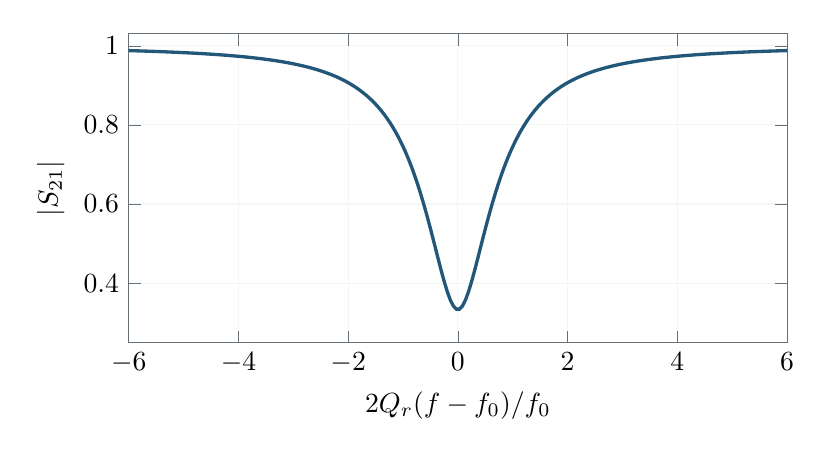
\begin{tikzpicture}
\begin{axis}[
  width=0.82\textwidth,height=5.5cm,
  xlabel={$2Q_r(f-f_0)/f_0$},ylabel={$|S_{21}|$},
  xmin=-6,xmax=6,ymin=0.25,ymax=1.03,
  grid=major,grid style={draw=KidGray},
  axis line style={draw=KidDark!70},tick style={draw=KidDark!70}
]
\addplot[KidBlue,very thick,domain=-6:6,samples=220]
  {sqrt(((1-0.6666667)^2+x^2)/(1+x^2))};
\end{axis}
\end{tikzpicture}
\end{center}

这里取 $Q_i=10^5,Q_c=5\times10^4$，因此 $d=Q_r/Q_c\approx2/3$。曲线的“深度”和“宽度”不是同一个信息：宽度主要给 $Q_r$，深度/圆直径再帮助分解 $Q_c$ 与 $Q_i$。

\section{为什么复数 $S_{21}$ 会形成一个圆？}

把上式分解成实部与虚部：
\[
\operatorname{Re}S_{21}=1-\frac{d}{1+y^2},
\qquad
\operatorname{Im}S_{21}=\frac{dy}{1+y^2}.
\]
消去 $y$ 可得
\[
\boxed{
\left(\operatorname{Re}S_{21}-\left(1-\frac d2\right)\right)^2
+
\left(\operatorname{Im}S_{21}\right)^2
=
\left(\frac d2\right)^2.
}
\]
因此理想 resonance 在 IQ 平面上严格是一条圆：
\begin{itemize}
  \item 圆心：$\left(1-d/2,0\right)$；
  \item 半径：$d/2$；
  \item far off resonance：$S_{21}\rightarrow1$；
  \item resonance point：$S_{21}(f_0)=1-d$。
\end{itemize}

\begin{center}
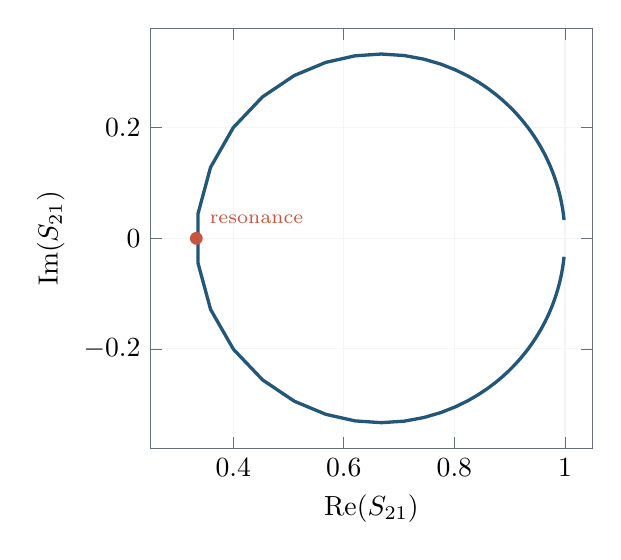
\begin{tikzpicture}
\begin{axis}[
  width=7.2cm,height=7.2cm,
  xlabel={Re$(S_{21})$},ylabel={Im$(S_{21})$},
  axis equal image,
  xmin=0.25,xmax=1.05,ymin=-0.38,ymax=0.38,
  grid=major,grid style={draw=KidGray},
  axis line style={draw=KidDark!70},tick style={draw=KidDark!70}
]
\addplot[KidBlue,very thick,domain=-20:20,samples=300,variable=\t]
  ({1-0.6666667/(1+\t^2)},{0.6666667*\t/(1+\t^2)});
\addplot[only marks,mark=*,mark size=2.1pt,KidRed] coordinates {(0.3333333,0)};
\node[font=\scriptsize,anchor=south west,text=KidRed] at (axis cs:0.34,0.01) {resonance};
\end{axis}
\end{tikzpicture}
\end{center}

这张圆不是画图技巧，而是一个非常有价值的拟合约束。真实 VNA 数据即使被放大、旋转、延迟，只要系统近似线性，resonance 轨迹仍然保留“圆结构”，这也是 circle fit 方法能够工作的原因。

\section{耦合强弱：不要只凭 notch 深浅判断“器件好不好”}

由
\[
\frac1{Q_r}=\frac1{Q_i}+\frac1{Q_c}
\]
可看出两种极限：

\subsection{$Q_c\gg Q_i$：feedline 耦合很弱}
此时
\[
Q_r\approx Q_i,
\qquad
\frac{Q_r}{Q_c}\ll1,
\]
因此 notch 很浅。器件可能内部损耗很低，也可能只是“几乎没耦合进去”。

\subsection{$Q_c\ll Q_i$：耦合损耗率占主导}
此时
\[
Q_r\approx Q_c,
\qquad
\frac{Q_r}{Q_c}\approx1,
\]
理想 lossless 极限下 resonance 可以接近零传输，notch 很深。

\begin{intuitionbox}
对于 hanger transmission geometry，与其在初学阶段机械套用“critical / under / over coupled”三个词，不如先问两个更不会错的问题：\textbf{内部损耗率大，还是 feedline 耦合率大？}以及\textbf{$Q_r$ 是被 $Q_i$ 限制，还是被 $Q_c$ 限制？}
\end{intuitionbox}

\section{KID 真正的读出：固定 probe tone，而不是不停扫 VNA}

扫频的主要作用是先找到 $f_0,Q_r,Q_c,Q_i$。真正观测时，我们通常在 resonance 附近固定一个或多个 readout tone，然后连续采集
\[
S_{21}(t)=I(t)+jQ(t).
\]

在一个工作点附近，可以线性化：
\[
\boxed{
\delta S_{21}
\approx
\frac{\partial S_{21}}{\partial f_0}\delta f_0
+
\frac{\partial S_{21}}{\partial(Q_i^{-1})}\delta(Q_i^{-1}).
}
\]
第一项主要来自 reactive / frequency response，第二项主要来自 dissipative response。

在 IQ 圆上可以形成一个很实用的几何直觉：
\begin{itemize}
  \item 改变 $f_0$，相当于让固定 probe tone 在 resonance 圆轨迹上“前后滑动”；
  \item 改变内部损耗，会同时改变圆的尺寸/位置和 probe point 到圆心的关系；
  \item 因而可以在局部定义近似正交的 frequency quadrature 与 dissipation quadrature。
\end{itemize}

\begin{center}
\begin{tikzpicture}[scale=1.05]
\draw[draw=KidDark!35] (0,0) circle (2.0cm);
\coordinate (C) at (0,0);
\coordinate (P) at (1.40,1.43);
\fill[KidBlue] (P) circle (2pt);
\draw[flowarrow] (P) -- ++(-0.72,0.70) node[above left,font=\scriptsize,text=KidBlue] {$\delta f_0$：沿切向为主};
\draw[goldarrow] (P) -- ++(0.72,0.72) node[above right,font=\scriptsize,text=KidGold!70!black] {$\delta Q_i^{-1}$：径向/形变为主};
\fill[KidDark] (C) circle (1.3pt) node[below,font=\scriptsize]{circle center};
\node[below right,font=\scriptsize,text=KidDark!70] at (P) {固定 probe 工作点};
\end{tikzpicture}
\end{center}

\begin{mistakebox}
“frequency direction 和 dissipation direction 永远严格正交”不是普遍定理。它们在经过正确归一化并在线性小信号附近可以构造为近似正交坐标；真实 cable delay、非对称耦合、噪声和非线性都会让几何关系偏离这张理想图。
\end{mistakebox}

\section{真实 VNA 数据为什么不是一个端正的圆？}

实验数据往往还叠加 readout chain：
\begin{itemize}
  \item cable delay 带来频率相关相位旋转；
  \item 放大器、衰减器、线缆带来 complex gain；
  \item 频率相关 baseline 让圆整体倾斜或拉伸；
  \item input/output impedance mismatch 可以产生 resonance asymmetry；
  \item 噪声让点云不再落在一条完美圆上。
\end{itemize}

一个常用的工程模型可以写成
\[
\boxed{
S_{21}^{\rm meas}(f)
=
G(f)e^{-j2\pi f\tau}
\left[
1-
\frac{(Q_r/Q_c)e^{j\phi}}
{1+2jQ_r(f-f_0)/f_0}
\right],
}
\]
其中
\begin{itemize}
  \item $G(f)$ 表示缓慢变化的 complex gain / baseline；
  \item $\tau$ 是 electrical delay；
  \item $\phi$ 是把 mismatch / asymmetry 吸收到一个有效复耦合角中的教学参数。
\end{itemize}

不同文献对 complex coupling quality factor 与 $\phi$ 的定义略有不同，所以真正复现 fitting code 时必须跟随所用模型的约定，不能只复制一个公式外形。

\section{一个可靠的 resonance fitting 流程}

面对一段真实 $S_{21}(f)$，建议按以下层级思考：

\begin{center}
\begin{tikzpicture}[node distance=7mm and 3.8mm]
\node[flowbox,fill=KidGray,minimum width=24mm] (raw) {raw complex\\$S_{21}(f)$};
\node[flowbox,right=of raw,minimum width=24mm] (delay) {估计/去除\\cable delay};
\node[flowbox,right=of delay,minimum width=25mm] (base) {complex gain\\baseline\\normalization};
\node[flowbox,right=of base,minimum width=24mm] (circle) {circle /\\line-shape fit};
\node[flowbox,right=of circle,minimum width=25mm] (par) {$f_0,Q_r,Q_c,Q_i$\\+ uncertainty};
\draw[flowarrow] (raw.east)--(delay.west);
\draw[flowarrow] (delay.east)--(base.west);
\draw[flowarrow] (base.east)--(circle.west);
\draw[flowarrow] (circle.east)--(par.west);
\end{tikzpicture}
\end{center}

最低限度的质量检查包括：
\begin{enumerate}
  \item 拟合残差是否随机，而不是还留着系统性弧形；
  \item 拟合窗口变宽/变窄时参数是否稳定；
  \item $Q_i,Q_c,Q_r$ 是否满足定义关系；
  \item 去 delay 前后 IQ 轨迹是否合理；
  \item 是否存在 nearby resonance、非线性、功率依赖或频率跳变。
\end{enumerate}

\section{为什么 resonance fitting 对 KID 比“普通滤波器”更重要？}

KID 的科学信号最终不是“有没有 notch”，而是小变化：
\[
\delta f_0(t),
\qquad
\delta Q_i^{-1}(t).
\]
如果 baseline、delay 或 coupling 模型错了，这些系统误差会直接投影成假的 optical response。

对于阵列还会进一步影响：
\begin{itemize}
  \item tone placement：probe tone 是否真的落在合适工作点；
  \item tone spacing：邻近 resonance 是否可能 collision；
  \item readout dynamic range：大量 tone 的 crest factor 与放大器线性区；
  \item tracking：光学负载变化后是否需要自动跟踪 $f_0$。
\end{itemize}

这就是为什么 $Q$、IQ circle 和 fitting 不是“读出工程的附属知识”，而是 detector calibration 本身。

\section{从 LEKID 仿真结果回到物理量}

\begin{projectbox}
在 Sonnet 平面电磁仿真中，更常直接看到 GHz 谐振响应。可将仿真结果按三个层级拆开：
\begin{enumerate}
  \item \textbf{geometry level：}meander + IDC + coupling 共同决定 $L,C$ 与耦合强度；
  \item \textbf{resonator level：}从复数 $S_{21}$ 拟合 $f_0,Q_r,Q_c,Q_i$；
  \item \textbf{material / detector level：}只有当超导薄膜模型包含真实 $Z_s$ / $L_k$ / loss 时，$Q_i$ 与 $f_0$ 才能继续往材料参数和光学响应解释。
\end{enumerate}
因此以后不建议只报“谐振在 \SI{2.5}{GHz}、notch 很深”，而应至少输出 $f_0,Q_r,Q_c$，并说明 $Q_i$ 是否物理可信、材料模型是否允许解释它。
\end{projectbox}

\section{配套 Python：从理想谐振到带失真的合成 VNA 数据}

本章配套两个可直接运行的示例：
\begin{itemize}
  \item \texttt{examples/resonator\_basics.py}：生成理想 notch、IQ circle、光照导致的 $f_0$ 位移与固定 tone IQ 位移；
  \item \texttt{examples/resonator\_fit\_demo.py}：给理想 resonance 加入 complex gain、cable delay、asymmetry 和复高斯噪声，再用非线性 least-squares 拟合回 $f_0,Q_r,Q_c,\phi,\tau$ 等参数。
\end{itemize}

建议先不看 fitting 脚本实现，自己完成第一个脚本中的四个 TODO，再运行参考版本对照。

\section{本章 2--3 小时学习任务}

\begin{enumerate}
  \item 从 $Q=\omega_0U/P_{loss}$ 独立推导 $1/Q_r=1/Q_i+1/Q_c$；
  \item 用 $f_0=\SI{2.5}{GHz},Q_i=10^5,Q_c=5\times10^4$ 算出 $Q_r,\Delta f,\tau_E,\tau_A$；
  \item 从 ideal $S_{21}$ 推导 IQ 圆方程，亲手证明圆心为 $1-d/2$、半径为 $d/2$；
  \item 运行 \texttt{resonator\_basics.py}，改变 $Q_i/Q_c$，观察 notch depth、linewidth 和圆直径分别怎么变化；
  \item 将 $f_0$ 人为移动 $-10$、$-30$、$-100\,\mathrm{kHz}$，比较固定 probe tone 的 $\Delta I,\Delta Q$；
  \item 运行 synthetic fitting 示例，分别关掉 cable delay、asymmetry、noise，观察每一种非理想项对 recovered $Q_i$ 的影响；
  \item 最后闭卷回答：\textbf{为什么只看 $|S_{21}|$ 不如同时拟合复数 $S_{21}$？}
\end{enumerate}

\section{闭卷理解检查}

\begin{checkpointbox}
\begin{enumerate}
  \item $Q_i,Q_c,Q_r$ 分别对应什么物理通道？
  \item 为什么独立损耗通道是 $1/Q$ 相加，而不是 $Q$ 相加？
  \item $Q_r$ 增大一倍时 linewidth 如何变化？
  \item energy lifetime 与 amplitude lifetime 为什么相差 2？
  \item ideal hanger $S_{21}$ 为什么在复平面是一条圆？
  \item notch 很浅时，为什么不能立刻判断器件内部损耗很大？
  \item 固定 probe tone 为什么能把 $\delta f_0$ 变成 $\delta I,\delta Q$？
  \item cable delay 在 IQ 平面最主要造成什么变化？
  \item 为什么 resonance asymmetry 会让简单的“旋转圆”方法偏置 $Q_i$？
  \item 对于 Sonnet 仿真结果，哪些 $Q$ 可以直接从 $S_{21}$ 得到，哪些解释依赖真实超导材料模型？
\end{enumerate}
\end{checkpointbox}

\begin{formula}[title=\bfseries 本章的一句话]
\centering
\[
\boxed{
(Q_i,Q_c)
\rightarrow
Q_r
\rightarrow
(\Delta f,\tau)
\rightarrow
S_{21}(f)
\rightarrow
\text{IQ circle}
\rightarrow
\text{fixed-tone }I/Q
}
\]
\end{formula}


\part{从光学响应到 LEKID 电磁设计}
\chapter{光学响应、噪声与 NEP：把“看到光”变成一个可比较的灵敏度指标}
\chapterguide
{“能看到 notch 变化”还不等于探测器灵敏；需要把光功率变化、输出变化和噪声放进同一套定量语言。}
{准粒子寿命、$S_{21}$ / IQ 读出，以及功率谱密度的基本概念。}
{从吸收功率走到 responsivity；区分 PSD/ASD；理解 photon、GR、TLS、amplifier noise，并把输出噪声折算为 NEP。}
{NEP 的本质，是把输出端噪声除以响应度，折回成等效输入光功率噪声。}

\begin{goalbox}
学完本章后，你应该能够把一颗 KID 的光学响应写成一条可计算的链：
\[
P_{\rm abs}\rightarrow \Gamma_{\rm qp}\rightarrow N_{\rm qp}\rightarrow
\delta f_0,\delta Q_i^{-1}\rightarrow \delta I,\delta Q,
\]
并能够回答：
\begin{enumerate}
  \item responsivity 到底是“对什么量求导”；
  \item 为什么 quasiparticle lifetime 同时决定信号增益和响应速度；
  \item PSD、ASD 与 NEP 的单位分别是什么；
  \item photon、generation--recombination、TLS、amplifier noise 在频谱上通常长什么样；
  \item 怎样判断一颗 KID 是否接近 photon-noise limited。
\end{enumerate}
\end{goalbox}

\section{先把这一章放回整条 KID 链}

前面的章节主要解决了“材料变化怎样变成 GHz 复数 $S_{21}$”。本章第一次把输入端的光功率和输出端的噪声统一起来：

\begin{center}
\begin{tikzpicture}[node distance=9mm and 4mm]
\node[flowbox,fill=KidGold!22,minimum width=23mm] (p) {$P_{\rm abs}$\\吸收光功率};
\node[flowbox,right=of p,minimum width=24mm] (g) {$\Gamma_{\rm qp}$\\准粒子产生率};
\node[flowbox,right=of g,minimum width=23mm] (n) {$N_{\rm qp}$\\稳态与涨落};
\node[flowbox,right=of n,minimum width=25mm] (r) {$f_0,Q_i$\\谐振器响应};
\node[flowbox,right=of r,minimum width=23mm] (iq) {$I,Q$\\数字读出};
\draw[goldarrow] (p.east)--(g.west);
\draw[flowarrow] (g.east)--(n.west);
\draw[flowarrow] (n.east)--(r.west);
\draw[flowarrow] (r.east)--(iq.west);
\node[flowbox,fill=KidRed!5,below=14mm of n,text width=38mm] (noise) {随机涨落\\photon / GR / TLS / amplifier};
\draw[influence] (noise.north) -- (n.south);
\draw[influence] (noise.north east) to[bend left=18] (iq.south west);
\end{tikzpicture}
\end{center}

\begin{intuitionbox}
responsivity 回答的是“输入改变一点，输出平均值改变多少”；noise 回答的是“即使输入不变，输出自己会抖多少”。NEP 做的事情，就是把输出端的抖动除以 responsivity，重新折算成输入端等效的功率抖动。
\end{intuitionbox}

\section{从吸收光功率到 quasiparticle generation rate}

设真正沉积在超导吸收体中的功率为 $P_{\rm abs}$。注意它已经包含了光学链上的耦合、反射、偏振匹配等结果，不应与望远镜口径处的 incident power 混为一谈。

光子能量最终只有一部分进入可观测的 quasiparticle population。用 pair-breaking efficiency $\eta_{\rm pb}$ 表示这一比例。若每个 quasiparticle 的典型激发能量尺度取 $\Delta$，最常用的工程近似是
\[
\boxed{\Gamma_{\rm qp}\simeq \frac{\eta_{\rm pb}P_{\rm abs}}{\Delta}}
\]
其中 $\Gamma_{\rm qp}$ 的单位是 \si{s^{-1}}。

这个式子不要误读为“一个光子只产生一个 quasiparticle”。一个高于 $2\Delta$ 的光子会触发 pair breaking 和后续 phonon cascade；$\eta_{\rm pb}$ 把复杂能量级联压缩成一个有效参数。

\begin{mistakebox}
$P_{\rm abs}$、incident optical power 和 readout microwave power 是三种不同的功率。前两者属于被探测的光学链，最后一个是 GHz probe tone。把它们混写成一个 $P$ 是 KID 推导里很常见的错误。
\end{mistakebox}

\section{稳态 quasiparticle 数：为什么 lifetime 会提高响应}

在小扰动附近，可以把复杂的 recombination 动力学线性化为
\[
\frac{dN_{\rm qp}}{dt}=\Gamma_{\rm qp}-\frac{N_{\rm qp}-N_{\rm qp,0}}{\tau_{\rm qp}}.
\]
若只关注额外光生 population，并假设 $\tau_{\rm qp}$ 在工作点附近近似常数，则稳态有
\[
\boxed{
\delta N_{\rm qp}
\simeq
\frac{\eta_{\rm pb}\tau_{\rm qp}}{\Delta}
\,\delta P_{\rm abs}
}
\]
于是
\[
\boxed{
\frac{\partial N_{\rm qp}}{\partial P_{\rm abs}}
\simeq
\frac{\eta_{\rm pb}\tau_{\rm qp}}{\Delta}
}
\]

这给出一个非常重要的器件直觉：\textbf{更长的 $\tau_{\rm qp}$ 会让同样的光功率在器件里积累更多 quasiparticle，因此静态 responsivity 往往更高。}

但它不是免费的，因为更长的 lifetime 同时意味着更慢的响应。

\section{从 $N_{\rm qp}$ 到 frequency / dissipation responsivity}

定义 fractional frequency shift
\[
x\equiv \frac{\delta f_0}{f_0}.
\]
在某个固定工作点附近，先不强迫自己每次都重新计算完整 Mattis--Bardeen 积分，而是定义材料-几何转换系数
\[
\mathcal K_x\equiv \frac{\partial x}{\partial N_{\rm qp}},
\qquad
\mathcal K_d\equiv
\frac{\partial Q_i^{-1}}{\partial N_{\rm qp}}.
\]
对于通常的 KID，$\mathcal K_x<0$，因为 quasiparticle 增多导致 $\sigma_2$ 下降、$L_k$ 增大、$f_0$ 下降；而 $\mathcal K_d>0$，因为耗散增加。

于是光功率 responsivity 为
\[
\boxed{
\mathcal R_x
\equiv
\frac{\partial x}{\partial P_{\rm abs}}
=\mathcal K_x
\frac{\eta_{\rm pb}\tau_{\rm qp}}{\Delta}
}
\]
以及
\[
\boxed{
\mathcal R_d
\equiv
\frac{\partial Q_i^{-1}}{\partial P_{\rm abs}}
=\mathcal K_d
\frac{\eta_{\rm pb}\tau_{\rm qp}}{\Delta}
}.
\]

如果需要更显式地接回 Mattis--Bardeen，常见小信号形式可写成
\[
\frac{\delta f_0}{f_0}
\propto
-\frac{\alpha S_2}{N_0\Delta V}\,\delta N_{\rm qp},
\]
\[
\delta Q_i^{-1}
\propto
\frac{\alpha S_1}{N_0\Delta V}\,\delta N_{\rm qp},
\]
其中 $S_1,S_2$ 是由温度与读出频率决定的 Mattis--Bardeen response factors。不同文献对 $N_0$、spin degeneracy 和几何因子约定不同，因此第一次使用具体 prefactor 时一定核对定义。

\section{再往前一步：从 responsivity 到真正的 $I/Q$ responsivity}

上一章已经有
\[
\delta S_{21}
\simeq
\frac{\partial S_{21}}{\partial f_0}\delta f_0
+
\frac{\partial S_{21}}{\partial Q_i^{-1}}\delta Q_i^{-1}.
\]
因此
\[
\boxed{
\frac{\partial S_{21}}{\partial P_{\rm abs}}
=
\frac{\partial S_{21}}{\partial f_0}
\frac{\partial f_0}{\partial P_{\rm abs}}
+
\frac{\partial S_{21}}{\partial Q_i^{-1}}
\frac{\partial Q_i^{-1}}{\partial P_{\rm abs}}
}
\]
就是 fixed-tone readout 最直接的复数 responsivity。

写成
\[
S_{21}=I+jQ,
\]
就得到两个实数：
\[
\mathcal R_I=\frac{\partial I}{\partial P_{\rm abs}},
\qquad
\mathcal R_Q=\frac{\partial Q}{\partial P_{\rm abs}}.
\]
工程上更常做的是先把 $(I,Q)$ 旋转到 frequency / dissipation 两个近似正交的坐标，再在这两个坐标里分别做 responsivity 和 noise analysis。

\section{时间响应：$\tau_{\rm qp}$ 与 resonator ring-down 谁更慢？}

若 optical power 有一个小的正弦调制 $\delta P e^{j2\pi ft}$，quasiparticle population 的一阶响应是
\[
H_{\rm qp}(f)=\frac{1}{1+j2\pi f\tau_{\rm qp}}.
\]
对应的 $-3\,\mathrm{dB}$ 截止频率：
\[
\boxed{f_{\rm qp}=\frac{1}{2\pi\tau_{\rm qp}}}.
\]

但读出端的 resonator 自己也有有限 ring-down。用上一章的 amplitude lifetime
\[
\tau_A=\frac{2Q_r}{\omega_0}
=\frac{Q_r}{\pi f_0},
\]
可把其基带响应也近似成一个低通环节。

因此一个最小动态模型是
\[
H_{\rm det}(f)
\simeq
\frac{1}{1+j2\pi f\tau_{\rm qp}}
\frac{1}{1+j2\pi f\tau_A}.
\]

\begin{projectbox}
假设你的读出 resonance 在 \SI{2.5}{GHz}，$Q_r=3.3\times10^4$，则 $\tau_A\approx\SI{4.2}{\micro s}$；若低温 Al 的有效 quasiparticle lifetime 是 \SI{300}{\micro s}，那么 detector bandwidth 主要由 quasiparticle 动力学而不是 resonator 限制。反过来，如果未来做极快 pulse detector 或故意把 $Q_r$ 做得非常高，ring-down 就可能进入瓶颈。
\end{projectbox}

\section{Noise PSD 与 ASD：先把单位彻底理顺}

若某个读出量 $y(t)$ 的单边功率谱密度记作 $S_y(f)$，单位是
\[
[y]^2/\mathrm{Hz}.
\]
其 amplitude spectral density 是
\[
\sqrt{S_y(f)},
\]
单位是
\[
[y]/\sqrt{\mathrm{Hz}}.
\]

例如 fractional frequency noise
\[
x(t)=\frac{\delta f_0(t)}{f_0}
\]
是无量纲量，因此
\[
S_x(f):\quad \mathrm{Hz}^{-1},
\qquad
\sqrt{S_x(f)}:\quad \mathrm{Hz}^{-1/2}.
\]

若直接用 frequency fluctuation $\delta f_0(t)$，则
\[
\sqrt{S_f}:\quad \mathrm{Hz}/\sqrt{\mathrm{Hz}}.
\]

\section{NEP：把输出噪声折回输入端}

如果选择 $x=\delta f_0/f_0$ 作为 detector observable，则
\[
\mathcal R_x=\frac{dx}{dP_{\rm abs}}
\]
单位为 \si{W^{-1}}。于是 input-referred NEP 定义为
\[
\boxed{
\mathrm{NEP}(f)
=
\frac{\sqrt{S_x(f)}}{|\mathcal R_x(f)|}
}
\]
单位自然是
\[
\boxed{\mathrm{W}/\sqrt{\mathrm{Hz}}}.
\]

同理，如果你使用 phase、$I$、$Q$ 或 dissipation channel，只要 noise 和 responsivity 使用同一个 observable，最后都可以换算成 NEP。

\begin{intuitionbox}
NEP 不是“输出噪声有多小”，而是“多小的输入功率涨落能够产生和现有输出噪声一样大的信号”。因此没有 responsivity，单独报一个 IQ noise 数字并不能说明 detector 灵敏度。
\end{intuitionbox}

\section{Photon noise：输入光本身就是随机的}

对于中心频率 $\nu$、吸收功率 $P_{\rm abs}$、等效光学带宽 $\Delta\nu$ 的单模近似，常见表达式是
\[
\boxed{
\mathrm{NEP}_{\rm ph}^2
\simeq
2h\nu P_{\rm abs}
+
\frac{2P_{\rm abs}^2}{\Delta\nu}
}
\]
第一项是 photon shot noise，第二项来自 thermal bunching / wave noise。

在低 occupancy 条件下，第一项常占主导：
\[
\mathrm{NEP}_{\rm shot}
\simeq
\sqrt{2h\nu P_{\rm abs}}.
\]

真正的多模、多偏振、宽带系统需要对 bandpass 和 occupation number 积分；上式的作用是建立量级和物理来源，而不是替代完整 optical model。

\section{Generation--recombination noise：quasiparticle 数自己也会涨落}

quasiparticle 的产生和复合是随机过程，因此即使平均 $N_{\rm qp}$ 不变，也会有 number fluctuation。在线性化模型和一种常用单边 PSD 约定下，低频 quasiparticle-number noise 可写为
\[
S_N(f)
\simeq
\frac{4N_{\rm qp}\tau_{\rm qp}}
{1+(2\pi f\tau_{\rm qp})^2}.
\]

利用
\[
\frac{dN_{\rm qp}}{dP_{\rm abs}}
\simeq
\frac{\eta_{\rm pb}\tau_{\rm qp}}{\Delta},
\]
可得到低频 input-referred GR noise 的常见形式
\[
\boxed{
\mathrm{NEP}_{\rm GR}
\simeq
\frac{2\Delta}{\eta_{\rm pb}}
\sqrt{\frac{N_{\rm qp}}{\tau_{\rm qp}}}
}.
\]
如果 quasiparticle population 主要由该 optical load 产生，并使用前述线性稳态关系，则进一步有
\[
\mathrm{NEP}_{\rm GR}^2
\simeq
\frac{4\Delta P_{\rm abs}}{\eta_{\rm pb}}.
\]
不同文献对 one-sided / two-sided PSD、$N_0$ 和 generation event 的定义会带来 factor-of-two 差别，所以比较数值时必须先对齐 convention。

\section{TLS noise：为什么低频 frequency channel 常常变“粉红”}

Two-Level Systems 通常与非晶介质、界面、电场集中的 capacitor 区域有关。它对 KID 最典型的影响不是简单增加一个白噪声底，而是造成低频 excess frequency noise，经验上常近似写作
\[
S_x^{\rm TLS}(f)\propto f^{-\beta},
\qquad \beta\sim 0.5\text{--}1,
\]
具体指数依器件、温度与 readout power 而变。

TLS 噪声通常具有几个工程特征：
\begin{itemize}
  \item 在低 Fourier frequency 更强；
  \item 对 capacitor 电场分布和介质参与比敏感；
  \item 增加 readout power 往往能在一定范围内使 TLS 饱和、降低其相对噪声；
  \item 但 readout power 过高又会进入 kinetic-inductance nonlinearity、heating 或 bifurcation。
\end{itemize}

这也是为什么 IDC 几何不是只负责“把谐振频率调到某个 GHz”，它还可能直接影响最终 noise floor。

\section{Amplifier / readout noise：它发生在 detector 之后}

低温 HEMT、室温放大器、ADC 量化与数字链都会给 $I/Q$ 添加噪声。理想放大器噪声在窄带基带里通常近似为白噪声。

它与 photon / GR noise 的关键区别是：\textbf{它并没有真的改变 $N_{\rm qp}$，而是污染了我们对 $S_{21}$ 的测量。}

因此 input-referred amplifier NEP 应写成
\[
\mathrm{NEP}_{\rm amp}(f)
=
\frac{\sqrt{S_{y,\rm amp}(f)}}
{|dy/dP_{\rm abs}|},
\]
其中 $y$ 可以选 frequency quadrature、phase 或某个最优线性组合。

提高 readout power 可以改善 amplifier-limited SNR，但最终会受到 resonator nonlinearity 和 detector back-action 的限制，所以“readout tone 越强越好”是不成立的。

\section{一个 150 GHz Al LEKID 的量级例子}

取一个用于建立量级感的工作点：
\[
\nu=\SI{150}{GHz},\qquad
T_c=\SI{1.2}{K},\qquad
P_{\rm abs}=\SI{1}{pW},
\]
\[
\eta_{\rm pb}=0.57,\qquad
\tau_{\rm qp}=\SI{300}{\micro s}.
\]
弱耦合 BCS 给出
\[
\Delta\simeq1.764k_BT_c\simeq\SI{0.182}{meV}.
\]
于是线性稳态估计
\[
N_{\rm qp}
\simeq
\frac{\eta_{\rm pb}P_{\rm abs}\tau_{\rm qp}}{\Delta}
\approx 5.9\times10^6.
\]

photon shot-noise 量级：
\[
\mathrm{NEP}_{\rm shot}
\approx
\sqrt{2h\nu P_{\rm abs}}
\approx
1.4\times10^{-17}\,\mathrm{W}/\sqrt{\mathrm{Hz}}.
\]
在相同近似与 PSD convention 下，GR noise 也得到约
\[
\mathrm{NEP}_{\rm GR}
\approx
1.4\times10^{-17}\,\mathrm{W}/\sqrt{\mathrm{Hz}}.
\]

这个“恰好同量级”不是所有 KID 的普遍定律，但它说明：在设计得不错的 pair-breaking detector 中，GR noise 本来就可能靠近 photon noise，而不是比它小很多个数量级。

\section{怎样做真正的 noise budget？}

如果各噪声源近似独立，则 input-referred noise 可按功率相加：
\[
\boxed{
\mathrm{NEP}_{\rm tot}^2(f)
=
\mathrm{NEP}_{\rm ph}^2
+
\mathrm{NEP}_{\rm GR}^2
+
\mathrm{NEP}_{\rm TLS}^2(f)
+
\mathrm{NEP}_{\rm amp}^2(f)
+\cdots
}
\]

工程上不应该只给一个“最小 NEP”，而应画出 NEP versus Fourier frequency。因为 detector 可能在 \SI{100}{Hz} 附近 photon-noise limited，却在 \SI{0.1}{Hz} 被 TLS / $1/f$ drift 完全支配。

\begin{center}
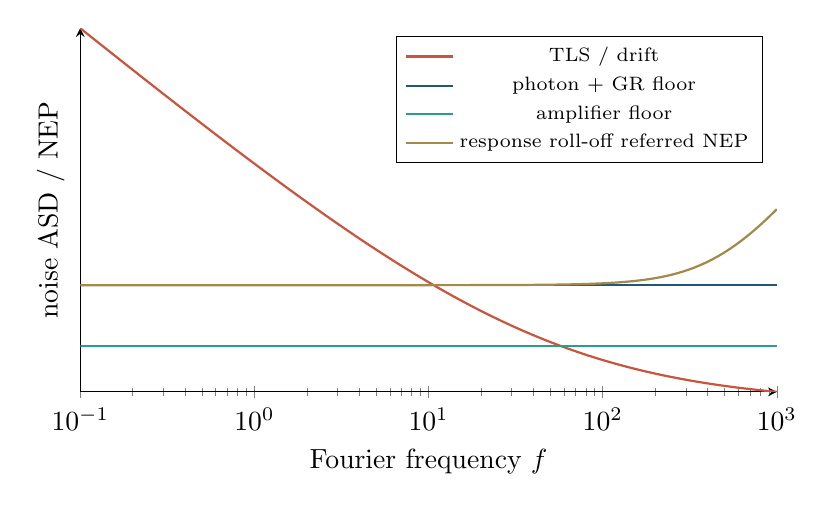
\begin{tikzpicture}
\begin{axis}[
width=0.86\textwidth,height=6.2cm,
xmode=log,ymode=log,
xlabel={Fourier frequency $f$},ylabel={noise ASD / NEP},
xtick={0.1,1,10,100,1000},
ytick=\empty,
legend style={font=\scriptsize,at={(0.98,0.98)},anchor=north east},
axis lines=left]
\addplot[KidRed,thick,domain=0.1:1000,samples=120] {1.4/x^0.65+0.12};
\addlegendentry{TLS / drift}
\addplot[KidBlue,thick,domain=0.1:1000,samples=80] {0.42};
\addlegendentry{photon + GR floor}
\addplot[KidTeal,thick,domain=0.1:1000,samples=80] {0.22};
\addlegendentry{amplifier floor}
\addplot[KidGold!70!black,thick,domain=0.1:1000,samples=120] {0.42*sqrt(1+(x/500)^2)};
\addlegendentry{response roll-off referred NEP}
\end{axis}
\end{tikzpicture}
\end{center}

这张图是概念示意，不对应某个具体器件；它要表达的是：\textbf{“噪声大小”必须和 Fourier frequency 绑定。}

\section{什么叫 photon-noise limited？}

一个实用判据不是“总 NEP 等于理论 photon NEP 到最后一位”，而是在目标科学频带内满足
\[
\mathrm{NEP}_{\rm other}^2
\ll
\mathrm{NEP}_{\rm ph}^2,
\]
使得
\[
\mathrm{NEP}_{\rm tot}
\approx
\mathrm{NEP}_{\rm ph}
\]
并且随着 optical loading 变化呈现合理的 photon-noise scaling。

真正有说服力的验证通常包括：
\begin{enumerate}
  \item blackbody / optical load 改变时测 $f_0$ 与 $Q_i$，得到 responsivity；
  \item 对同一工作点记录长时间 $I/Q$ timestream；
  \item 转成 frequency / dissipation noise PSD；
  \item 用 measured responsivity 折算 NEP；
  \item 与 photon + GR + readout noise model 比较；
  \item 改变 optical loading、bath temperature 和 readout power，检查 scaling 是否一致。
\end{enumerate}

\section{工程案例：双偏振 150 GHz LEKID}

\begin{projectbox}
对于双偏振 150 GHz LEKID，可把器件性能拆成四层，而不只看 absorption 或 notch：
\begin{enumerate}
  \item \textbf{Optical layer：}$A_X(\nu,\theta),A_Y(\nu,\theta)$，得到每个偏振真正的 $P_{\rm abs}$；
  \item \textbf{Material layer：}$P_{\rm abs}\rightarrow N_{\rm qp}\rightarrow\delta\sigma_1,\delta\sigma_2$；
  \item \textbf{Resonator layer：}$\delta\sigma\rightarrow\delta f_0,\delta Q_i^{-1}\rightarrow\delta I/Q$；
  \item \textbf{Sensitivity layer：}responsivity + noise PSD $\rightarrow$ NEP。
\end{enumerate}
因此比较 B0 / B1 backshort 时，最终问题不应只是“谁吸收率高”，还应比较在给定 sky loading 下的端到端响应度、NEP 与双偏振对称性。这样才能从单纯的电磁吸收比较升级为完整的探测器研究问题。
\end{projectbox}

\section{配套 Python：光学响应与噪声预算}

本章配套两个示例：
\begin{itemize}
  \item \texttt{examples/optical\_responsivity\_demo.py}：从 $P_{\rm abs}$ 计算 $N_{\rm qp}$，再用一个可替换的 $dx/dN_{\rm qp}$ calibration coefficient 生成 fractional frequency response，并画出 quasiparticle lifetime 对响应速度的影响；
  \item \texttt{examples/noise\_budget\_demo.py}：计算 150 GHz 下的 photon shot / bunching noise、GR noise，并演示如何把一个 measured fractional-frequency noise ASD 用 responsivity 折算成 NEP。
\end{itemize}

\section{本章 3--4 小时学习任务}

\begin{enumerate}
  \item 从 $\Gamma_{\rm qp}=\eta_{\rm pb}P_{\rm abs}/\Delta$ 和一阶 lifetime 模型推导 $dN_{\rm qp}/dP_{\rm abs}$；
  \item 用本章 Al 数值例子独立算一遍 $\Delta,N_{\rm qp},\mathrm{NEP}_{\rm shot},\mathrm{NEP}_{\rm GR}$；
  \item 证明 NEP 的单位一定是 \si{W/\sqrt{Hz}}；
  \item 画出 $|H_{\rm qp}(f)|$，把 $\tau_{\rm qp}$ 从 \SI{30}{\micro s} 改到 \SI{3}{ms}，观察 bandwidth；
  \item 假设一个 measured $\sqrt{S_x}=10^{-9}/\sqrt{\mathrm{Hz}}$ 和 $|dx/dP|=10^6\,\mathrm{W^{-1}}$，计算 detector NEP；
  \item 运行 noise budget 脚本，改变 $P_{\rm abs}$ 与 $\Delta\nu$，观察 shot / bunching / GR 三项怎样缩放；
  \item 最后闭卷回答：\textbf{为什么“响应很大”不等于“NEP 很好”？}
\end{enumerate}

\section{闭卷理解检查}

\begin{checkpointbox}
\begin{enumerate}
  \item $\eta_{\rm pb}$ 在物理上压缩了哪些复杂过程？
  \item 为什么 $\tau_{\rm qp}$ 增大会提高静态 responsivity，却降低动态带宽？
  \item frequency responsivity 与 $I/Q$ responsivity 有什么区别？
  \item PSD 和 ASD 的单位为什么相差一个平方根？
  \item NEP 为什么必须通过同一 observable 的 responsivity 来 input-refer？
  \item photon shot noise 与 bunching noise 分别怎样随 $P_{\rm abs}$ 缩放？
  \item GR noise 是发生在 readout amplifier 之前还是之后？
  \item TLS 为什么经常首先污染低 Fourier frequency 的 frequency channel？
  \item 为什么提高 readout power 可以改善 amplifier-limited SNR，却不能无限提高？
  \item 你要证明一颗 KID photon-noise limited，至少需要做哪些 loading / PSD / responsivity 测量？
\end{enumerate}
\end{checkpointbox}

\begin{formula}[title=\bfseries 本章的一句话]
\centering
\[
\boxed{
P_{\rm abs}
\rightarrow N_{\rm qp}
\rightarrow (f_0,Q_i)
\rightarrow I/Q,
\qquad
\mathrm{NEP}=\frac{\text{output noise ASD}}{\text{responsivity}}
}
\]
\end{formula}


\chapter[LEKID 电磁设计]{LEKID 电磁设计：把 absorber、resonator、polarization 与 backshort 放进同一个模型}
\chapterguide
{前面的材料与谐振器理论只有落到真实几何上，才会变成可加工、可吸收、可偏振选择、可读出的 LEKID。}
{第 3、5--7 章；熟悉 $L_k$、$Q_c$、表面阻抗和基本电磁边界条件会更顺畅。}
{解释 meander 的双频身份、IDC / coupling、sheet impedance、waveguide mode、偏振、backshort、solver 分工与 full-wave power closure。}
{LEKID 设计不是两个独立器件拼接，而是同一几何同时承担毫米波吸收和 GHz 谐振两套电磁任务。}

\begin{goalbox}
学完本章后，你应该能够把一颗 LEKID 拆成两套频率尺度完全不同、但由同一片金属几何连接起来的电磁系统，并回答：
\begin{enumerate}
  \item 为什么同一条 meander 在 \SI{150}{GHz} 是吸收器，在 \SIrange{1}{3}{GHz} 又是谐振器电感？
  \item 膜厚、线宽、线距、fill factor 为什么会同时改变 optical absorption、$L_k$、dynamic range 与 responsivity？
  \item IDC、coupling capacitor 与 feedline 分别控制 $f_0$、$Q_c$ 和 multiplexing 的哪一部分？
  \item 圆波导中的 TE$_{11}$、TM$_{01}$、TE$_{21}$ 为什么会影响偏振仿真与能量闭合？
  \item backshort 为什么常从 $\lambda/4$ 起步，却不能把 $\lambda/4$ 当成最终答案？
  \item Sonnet 与 CST/HFSS 应分别验证哪一层物理，哪些结果绝不能混着解释？
\end{enumerate}
\end{goalbox}

\section{第一原则：LEKID 是同一几何上的“两套电磁问题”}

一颗直接吸收式 LEKID 同时工作在至少两个相差约两个数量级的频率尺度：
\[
\boxed{
\text{毫米波 / 亚毫米波：光学吸收}
\qquad\text{与}\qquad
\text{GHz：谐振读出}
}
\]

以本讲义持续使用的 \SI{150}{GHz} 器件为例：
\[
\lambda_{150\,\mathrm{GHz}}\approx \SI{2}{mm},
\]
而若读出谐振频率为 \SI{1.5}{GHz}：
\[
\lambda_{1.5\,\mathrm{GHz}}\approx \SI{200}{mm}.
\]
几何尺度对两者的“电尺寸”完全不同。

\begin{center}
\begin{tikzpicture}[node distance=11mm and 13mm]
\node[flowbox,fill=KidGold!20,text width=42mm] (opt) {\textbf{150 GHz optical problem}\\waveguide / polarization\\sheet impedance / backshort\\absorption $A(\nu,\theta)$};
\node[flowbox,right=of opt,fill=KidBlue!7,text width=42mm] (mw) {\textbf{GHz resonator problem}\\meander $L_g+L_k$\\IDC $C$ / coupler $C_c$\\$f_0,Q_i,Q_c,S_{21}$};
\node[flowbox,below=14mm of $(opt)!0.5!(mw)$,fill=KidGray,text width=56mm] (geom) {同一片超导薄膜几何\\$w,g,t$、路径长度与材料 $Z_s(\omega)$};
\draw[influence] (geom.north west) to[bend left=10] (opt.south);
\draw[influence] (geom.north east) to[bend right=10] (mw.south);
\node[font=\scriptsize,below=2mm of geom,text=KidDark!80] {几何同时影响 optical current path 与 GHz 的 $L,C,Q$};
\end{tikzpicture}
\end{center}

\begin{intuitionbox}
在 \SI{150}{GHz}，你主要问“入射场怎样在 meander 中激起电流并耗散功率”；在 GHz，你主要问“这段 meander 与 IDC 一起储存多少磁场/动能与电场能量”。\textbf{同一条线，但问题的边界条件、材料模型、模态与可观测量不同。}
\end{intuitionbox}

\section{meander 的双重身份：absorber + kinetic inductor}

LEKID 最迷人的地方，也是最容易设计冲突的地方，就是吸收电感不是“先做一个 absorber，再接一个独立电感”，而是同一段金属同时承担两种功能。

\subsection{在 GHz：它主要贡献 $L_g+L_k$}

读出端仍然由
\[
f_0=\frac{1}{2\pi\sqrt{LC}}
\]
控制，其中
\[
L=L_g+L_k.
\]
增加 meander 路径长度通常会增加总电感；减小线宽、减小膜厚常会提高 kinetic inductance contribution，但也会改变 current density、critical current、nonlinearity 和 fabrication sensitivity。

\subsection{在 150 GHz：它是一张“稀疏的复阻抗薄膜”}

毫米波看到的不是一个抽象的 lumped $L$，而是一组周期/准周期金属条形成的复表面响应。最简工程模型可以先写成
\[
Z_{\rm eff}(\nu)=R_{\rm eff}(\nu)+jX_{\rm eff}(\nu).
\]
如果金属线宽为 $w$、周期约为 $p=w+g$，定义 fill factor
\[
F=\frac{w}{p},
\]
那么在一个非常粗略的“电流沿金属条方向流动”的均匀化模型下，可以把稀疏金属的有效电阻理解为
\[
R_{\rm eff}\sim \frac{R_{\square}}{F}.
\]
这里不是要求你把这个式子直接用于最终设计，而是建立直觉：\textbf{同样的薄膜 sheet resistance，可以通过几何 fill factor 显著改变自由空间/波导看到的有效阻抗。}

\begin{mistakebox}
$R_{\rm eff}\sim R_{\square}/F$ 只是第一遍均匀化直觉。真实 meander 是 anisotropic strip grid，存在几何电感、相邻线耦合、有限基底、waveguide mode、边缘电流和超导复电导；最终吸收必须以 full-wave 结果为准。
\end{mistakebox}

\section{为什么“提高 absorber 体积”会牵一发动全身}

对有较大 optical loading 的器件，常希望增加 absorber volume $V$，以降低同样吸收功率产生的 quasiparticle density，并避免 $Q_i$ 过快恶化。McCarrick 等人的 \SI{150}{GHz} 双偏振 LEKID 设计就是一个很直观的例子：通过把电感线做成 wiggle，增加有效长度和体积，同时尽量保持合适的毫米波表面阻抗。

对简单条带：
\[
V\approx lwt.
\]
所以你可以通过 $l,w,t$ 增大体积。但三种方法的副作用完全不同：
\begin{itemize}
  \item 增大 $t$：最直接增加体积，但会降低 normal/superconducting sheet impedance，可能破坏 optical matching；
  \item 增大 $w$：改变 fill factor、偏振选择性、current density 与 $L_k$；
  \item 增大 $l$：通常增加 GHz 电感、改变 $f_0$，也可能改变毫米波电流路径与交叉偏振；
  \item wiggle：可以在不显著扩大 aperture footprint 的情况下增加 $l$ 与 $V$，但会引入额外局部方向分量，因此必须重新检查 cross-pol。
\end{itemize}

\begin{projectbox}
hairpin / half-hairpin + wiggle 这类结构，本质上是在同时优化四件事：\textbf{active volume、毫米波有效阻抗、GHz 电感、偏振纯度}。因此不要把“wiggle 长度”只当成机械几何参数；它应同时进入 optical 与 microwave 两套参数扫描。
\end{projectbox}

\section{一个极简吸收模型：为什么 backshort 能把 50\% 上限推向 100\%}

先看一个故意简化的 toy model。假设一张零厚度电阻膜位于均匀介质中，没有 backshort。对称环境下，单张被动 resistive sheet 的最大吸收通常不会超过 50\%；原因是还有一个 transmission channel 可以带走能量。

加入理想 PEC backshort 后，透射通道被封死：
\[
T=0,
\]
于是
\[
A=1-|\Gamma|^2.
\]
把 absorber 看成 sheet impedance $Z_s$，背后是长度 $d$ 的短路传输线。短路 stub 的输入阻抗：
\[
Z_{\rm stub}=jZ_d\tan(\beta d).
\]
在
\[
\beta d=\frac{\pi}{2}
\]
即近似 quarter-wave 条件下，$Z_{\rm stub}\rightarrow\infty$，背后的 PEC 通过 $\lambda/4$ 变换成近似 open。此时前表面主要由 absorber sheet 本身决定。

如果前侧等效波阻抗为 $Z_0$，理想匹配要求大致满足
\[
\boxed{Z_s\approx Z_0,}
\]
于是
\[
\Gamma\approx0,\qquad A\approx1.
\]

\begin{intuitionbox}
backshort 不是“帮 absorber 多反射一次”这么简单。更准确的说法是：它通过相位条件把 absorber 所处的电磁边界条件重新塑造成一个 impedance matching problem。
\end{intuitionbox}

\section{为什么 $\lambda/4$ 只是起点，不是最终答案}

在折射率为 $n$ 的介质中，第一遍 quarter-wave 厚度是
\[
d_{\lambda/4}=\frac{\lambda_0}{4n}=\frac{c}{4n\nu}.
\]
取 silicon 的毫米波折射率近似 $n\approx3.4$，在 \SI{150}{GHz}：
\[
\lambda_0\approx\SI{2.00}{mm},
\qquad
d_{\lambda/4}\approx\SI{147}{\micro m}.
\]
这解释了为什么许多 \SI{150}{GHz} horn-coupled LEKID 结构会出现 \SI{150}{\micro m} 左右的 silicon thickness；McCarrick 等人的一类设计使用约 \SI{160}{\micro m} silicon wafer，并在背面金属化形成 backshort / ground plane。

但实际最优值会因为以下因素偏离：
\begin{itemize}
  \item absorber 本身有 $X_s\neq0$；
  \item waveguide 到 wafer 之间存在 vacuum gap；
  \item waveguide aperture / choke 改变局部 modal impedance；
  \item substrate 有有限厚度、有限损耗和可能的 standing-wave structure；
  \item meander 不是均匀 sheet；
  \item 入射角和偏振改变 effective electrical length；
  \item 多模传播时，不同 mode 的相位条件不同。
\end{itemize}

因此工程流程应当是
\[
\boxed{
\lambda/4\ \text{估算}
\rightarrow
\text{full-wave sweep}
\rightarrow
\text{band-integrated optimization}
}
\]
而不是“计算出 $147\,\mu$m 就结束”。

\section{圆波导：先知道哪些 mode 真正在传播}

对于半径 $a$、直径 $D=2a$ 的圆波导，模态截止频率为
\[
f_c=\frac{x\,c}{2\pi a}=\frac{x\,c}{\pi D},
\]
其中 TE mode 使用 $J_m'(x)=0$ 的根，TM mode 使用 $J_m(x)=0$ 的根。

常用前三组为：
\[
x'_{11}=1.8412,\qquad x_{01}=2.4048,\qquad x'_{21}=3.0542.
\]
所以
\[
\begin{aligned}
f_{c,\mathrm{TE}_{11}}&=\frac{1.8412c}{\pi D},\\
f_{c,\mathrm{TM}_{01}}&=\frac{2.4048c}{\pi D},\\
f_{c,\mathrm{TE}_{21}}&=\frac{3.0542c}{\pi D}.
\end{aligned}
\]

对 $D=\SI{1.6}{mm}$：
\[
\boxed{
\begin{aligned}
f_{c,\mathrm{TE}_{11}}&\approx\SI{109.8}{GHz},\\
f_{c,\mathrm{TM}_{01}}&\approx\SI{143.4}{GHz},\\
f_{c,\mathrm{TE}_{21}}&\approx\SI{182.1}{GHz}.
\end{aligned}}
\]

于是 \SIrange{149}{151}{GHz} 附近：
\begin{itemize}
  \item TE$_{11}$ 已传播；
  \item TM$_{01}$ 也已传播；
  \item TE$_{21}$ 仍截止。
\end{itemize}

\begin{projectbox}
这也解释了为什么 full-wave 能量闭合不能只看 TE$_{11}$ 的两个偏振分量：在 \SI{150}{GHz}、$D=\SI{1.6}{mm}$ 的圆波导里，TM$_{01}$ 已经是传播通道。若忽略它，$|S|^2$ 能量闭合可能看起来“凭空丢失”。
\end{projectbox}

\section{TE$_{11}$ 的两重简并：偏振在求解器里必须被明确固定}

圆波导基本模 TE$_{11}$ 有两个互相正交、截止频率相同的简并解。你可以把它们理解为同一空间场型旋转 $90^\circ$ 后的两个线偏振基。

\begin{center}
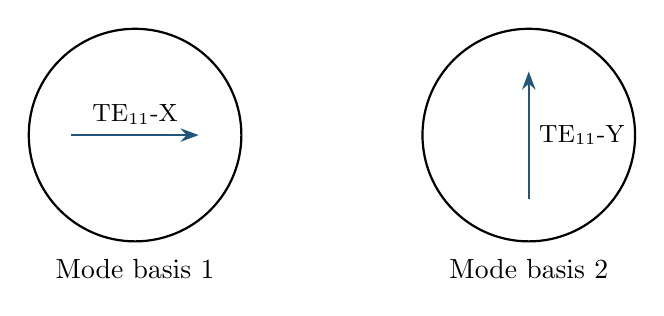
\begin{tikzpicture}[scale=1.0]
\draw[thick] (0,0) circle (1.35);
\draw[flowarrow] (-0.85,0)--(0.85,0) node[midway,above,font=\small]{TE$_{11}$-X};
\node at (0,-1.7) {Mode basis 1};
\begin{scope}[xshift=5cm]
\draw[thick] (0,0) circle (1.35);
\draw[flowarrow] (0,-0.85)--(0,0.85) node[midway,right,font=\small]{TE$_{11}$-Y};
\node at (0,-1.7) {Mode basis 2};
\end{scope}
\end{tikzpicture}
\end{center}

如果求解器没有固定 polarization angle / mode basis，那么不同 mesh、不同频点或不同设置下，简并子空间内的基矢可能发生旋转；这会让“X mode / Y mode”的 S 参数看起来难以比较。

因此偏振仿真必须明确记录：
\begin{enumerate}
  \item excitation mode index；
  \item polarization angle / field orientation；
  \item 每个 propagating reflected/transmitted mode；
  \item mode cutoff 与当前频段的关系。
\end{enumerate}

\section{怎样定义 co-pol、cross-pol 与 polarization efficiency}

设 X 偏振 resonator 的吸收功率为 $A_X$。对 X 入射：
\[
A_{XX}(\nu)=\frac{P_{\rm abs,X-res}}{P_{\rm inc,X}},
\]
而同一入射被 Y resonator 吸收的部分可以定义为
\[
A_{YX}(\nu)=\frac{P_{\rm abs,Y-res}}{P_{\rm inc,X}}.
\]
对 Y 入射同理得到 $A_{YY}$ 与 $A_{XY}$。

一个常用的直觉型 polarization selectivity 指标可以写成
\[
\eta_{p,X}=\frac{A_{XX}-A_{XY}}{A_{XX}+A_{XY}},
\]
注意不同论文可能采用不同定义，所以真正比较文献前一定要先看 definition。

对双偏振像元，至少要同时关心：
\begin{itemize}
  \item co-pol absorption：$A_{XX},A_{YY}$；
  \item cross-pol absorption：$A_{XY},A_{YX}$；
  \item 两偏振 bandshape mismatch；
  \item 随 incidence angle 的偏振不对称；
  \item 两个 resonator 之间的 microwave / optical crosstalk。
\end{itemize}

\begin{mistakebox}
“两个电感正交放置”只保证了第一阶偏振选择性，并不自动保证低 cross-pol。hairpin 的回转段、引线、IDC access line、开口边缘和 backshort/choke 都可能给另一偏振提供电流路径。
\end{mistakebox}

\section{为什么 hairpin end-turn 会影响 cross-pol}

设一条理想长直导线只沿 $x$ 方向，入射 $E_x$ 很容易驱动纵向电流，而 $E_y$ 的耦合较弱。但 hairpin 必然有 turn-around segment；这些局部线段包含 $y$ 向分量，于是会给正交偏振提供额外吸收通道。

这就是为什么真实双偏振 LEKID 设计中，经常需要对末端 meander / turn 做专门优化，而不是把两条正交长线简单叠放。McCarrick 等人的器件就专门对一组电感末端进行了 meander 调整，以降低 cross-polarization absorption。

\begin{projectbox}
在一种典型的非等价双偏振拓扑中，X 可采用 full hairpin，Y 可采用两个 half-hairpin 串联，并要求单层、无 crossover。这样的拓扑会使两偏振的 end-turn / access path 不完全等价。因此“几何四重对称”真正要验证的是\textbf{电流分布和吸收谱是否恢复近似对称}，而不只是 CAD 轮廓看起来对称。
\end{projectbox}

\section{IDC：它主要控制 GHz 电场，而不是 150 GHz 吸收}

在 lumped approximation 下，IDC 的主要任务是提供电容 $C$：
\[
f_0\approx\frac{1}{2\pi\sqrt{LC}}.
\]
一般地：
\begin{itemize}
  \item finger 越长，$C$ 越大，$f_0$ 越低；
  \item finger 数越多，$C$ 通常越大；
  \item gap 越小，局部电场越强，$C$ 增大，但 fabrication tolerance 与 TLS participation 也更敏感；
  \item IDC 周围 stray capacitance、grounding 和邻近 resonator 会造成 frequency pulling。
\end{itemize}

GHz 下，IDC gap 附近是高 electric-field participation 区域，因此 surface dielectric / native oxide / contamination 容易通过 TLS 影响 $Q_i$ 和 frequency noise。也就是说：
\[
\boxed{
\text{meander 更像 magnetic/kinetic energy region，IDC 更像 electric-field sensitive region。}
}
\]

\section{coupling capacitor 与 $Q_c$：不是 notch 越深越好}

feedline 与 resonator 之间的耦合决定 $Q_c$。对弱电容耦合的 lumped resonator，一个常见的近似形式是
\[
Q_c\propto\frac{C}{\omega_0 Z_0 C_c^2},
\]
不同具体拓扑会带来 1 或 2 等数值因子，所以设计时应使用与你的等效电路/EM topology 一致的公式或直接 full-wave 提取。

重要的是 scaling：
\[
C_c\uparrow\Rightarrow Q_c\downarrow\Rightarrow\text{coupling stronger}.
\]

但最优 $Q_c$ 不是无限小。对 detector array，你至少要平衡：
\begin{itemize}
  \item resonance visibility / readout SNR；
  \item optical load 下 $Q_i$ 会下降；
  \item loaded linewidth $f_0/Q_r$；
  \item resonator collision margin；
  \item readout power 与 bifurcation / nonlinearity；
  \item multiplexing density。
\end{itemize}

在很多设计中，会希望工作 optical load 下 $Q_c$ 与 $Q_i$ 同量级，而不是在 dark condition 下追求“最漂亮的 notch”。

\section{双偏振像元中的 microwave 隔离也必须单独检查}

两只 LEKID 在 optical aperture 中靠得很近，但它们的 GHz resonance frequency 应通过 IDC 设计错开。即使 optical coupling 很好，也可能出现：
\begin{itemize}
  \item mutual capacitance；
  \item mutual inductance；
  \item feedline-mediated coupling；
  \item avoided crossing；
  \item fabrication scatter 导致 resonance collision。
\end{itemize}

因此“偏振隔离”至少有两种完全不同的含义：
\[
\boxed{
\text{optical cross-pol isolation}
\neq
\text{microwave resonator isolation}
}
\]
这两项应分别仿真、分别测量。

\section{材料模型：PEC 在 150 GHz absorber 问题里会把吸收直接抹掉}

对于 GHz geometry study，把金属先当 PEC，有时还能回答：
\begin{itemize}
  \item 几何电感趋势；
  \item IDC capacitance；
  \item coupling topology；
  \item current path；
  \item parasitic coupling。
\end{itemize}

但对 \SI{150}{GHz} direct absorber，如果把 absorber 当 ideal PEC：
\[
R_s=0,
\]
则材料本身没有 ohmic/quasiparticle dissipation，求解器不会得到你真正需要的 detector absorption。

所以 optical model 中必须给 absorber 合理的 frequency-dependent complex response，例如：
\[
Z_s(\nu,T)=R_s+jX_s
\]
或等价的 complex conductivity / thin-film sheet impedance。尤其当 $h\nu>2\Delta$ 时，不能把 GHz 低频极限下的 $\sigma_2\gg\sigma_1$ 直觉原封不动搬到 150 GHz。

\section{Sonnet 与 CST/HFSS：不要让一个 solver 同时承担所有责任}

\begin{center}
\begin{tabularx}{0.96\linewidth}{>{\bfseries}p{28mm}XX}
\toprule
问题 & Sonnet / 2.5D planar EM 更擅长 & CST/HFSS / 3D full-wave 更擅长 \\
\midrule
GHz resonator & $f_0$、IDC、coupler、feedline、planar current、parasitics & 可做，但通常计算成本更高 \\
150 GHz optical & 只适合高度简化的 planar periodic/sheet 问题 & waveguide、horn、choke、vacuum gap、backshort、mode excitation、angle/polarization \\
材料 & sheet impedance / surface inductance 很方便 & frequency-dependent bulk/surface impedance、lossy thin film \\
偏振/模态 & 不适合真实 3D waveguide mode basis & TE/TM mode、cross-pol、modal S 参数、场分布 \\
阵列耦合 & planar microwave coupling & package / cavity / stray optical coupling \\
\bottomrule
\end{tabularx}
\end{center}

\begin{intuitionbox}
最稳妥的 multiscale workflow 不是“找一个最强 solver 全部算完”，而是\textbf{每个 solver 只回答它最擅长的问题，然后用可比较的中间量把结果接起来。}
\end{intuitionbox}

\section{150 GHz full-wave 仿真中怎样做能量闭合}

如果输入功率归一化为 1，一个包含多传播模态和有损 absorber 的模型，应满足
\[
\boxed{
1=P_{\rm refl}+P_{\rm trans}+P_{\rm abs}+P_{\rm other}
}
\]
其中封闭 backshort 结构通常 $P_{\rm trans}\approx0$。

如果端口存在多个 propagating modes：
\[
P_{\rm refl}=\sum_m |S_{m\leftarrow n}|^2
\]
必须对所有传播通道求和，而不是只看“同偏振反射”。

如果你直接从体/表面 loss integration 得到 absorber dissipated power，则还可以交叉验证
\[
A_{\rm abs}=\frac{P_{\rm loss,absorber}}{P_{\rm inc}}.
\]

\begin{checkpointbox}
一个可信的 full-wave optical result 至少应同时通过三道检查：
\begin{enumerate}
  \item propagating-mode power closure；
  \item absorber dissipated power 与 $1-|S|^2$ 的一致性；
  \item mesh / frequency sampling / port mode basis 的收敛与可重复性。
\end{enumerate}
\end{checkpointbox}

\section{不要只优化峰值吸收：应该优化 band-integrated detector objective}

天文器件通常不关心某一个频点的 $A=99.9\%$，而更关心整个 science band：
\[
\bar A=\frac{\int W(\nu)A(\nu)d\nu}{\int W(\nu)d\nu},
\]
其中 $W(\nu)$ 可以包含 filter bandpass、source spectrum、optical throughput 等权重。

对双偏振像元，还可以定义一个示意性的综合 merit function：
\[
\mathcal M=
\bar A_X+\bar A_Y
-\lambda_1\overline{A_{\rm cross}}
-\lambda_2\overline{|A_X-A_Y|}
-\lambda_3 P_{\rm angle},
\]
其中 $P_{\rm angle}$ 表示大入射角性能惩罚。这里的 $\lambda_i$ 不是物理常数，而是设计权重。

这比单独盯着某个 S 参数 notch 或某个中心频率 absorption 更接近真实器件优化。

\section{双偏振 150 GHz 工程案例的验证分层}

\begin{projectbox}
可将这类双偏振设计拆成以下五层：
\begin{enumerate}
  \item \textbf{Waveguide layer：}TE$_{11}$-X / TE$_{11}$-Y 激励，TM$_{01}$ 等传播通道闭合；
  \item \textbf{Optical absorber layer：}$A_{XX},A_{YY},A_{XY},A_{YX}$ 随 $\nu$、入射角与 backshort 参数变化；
  \item \textbf{Geometry symmetry layer：}full-hairpin / half-hairpin、wiggle、end-turn、access line 是否造成不对称 current hot spot；
  \item \textbf{GHz resonator layer：}Sonnet 中提取 $f_0,Q_c$、current distribution、IDC/coupler sensitivity；
  \item \textbf{Detector layer：}把 optical $P_{\rm abs}$ 送入前文的 responsivity / NEP model。
\end{enumerate}
因此 B0 / B1 backshort 的研究问题最终可以从“谁的 absorption 更高”升级成：\textbf{谁在带宽、入射角、双偏振对称性、cross-pol 与 end-to-end sensitivity 上更优。}
\end{projectbox}

\section{配套 Python 示例}

本版本新增：
\begin{itemize}
  \item \texttt{waveguide\_modes\_demo.py}：计算圆波导 TE$_{11}$、TM$_{01}$、TE$_{21}$ cutoff，并对 $D=\SI{1.6}{mm}$ 标出 \SIrange{149}{151}{GHz} 工作区；
  \item \texttt{backshort\_toy\_model.py}：用“resistive sheet + grounded dielectric transmission line”的 toy model 扫描 backshort thickness 与 sheet resistance，展示 quarter-wave matching 为什么出现，以及 absorber reactance 为什么会移动最佳厚度。
\end{itemize}

\section{本章 4 小时学习任务}

\begin{enumerate}
  \item 手算 $D=\SI{1.6}{mm}$ 圆波导的 TE$_{11}$、TM$_{01}$、TE$_{21}$ 截止频率；
  \item 用 $n_{\rm Si}=3.4$ 手算 \SI{150}{GHz} 的 quarter-wave silicon thickness；
  \item 解释为什么把 absorber 当 PEC 会让 direct-absorption simulation 失去物理意义；
  \item 用 $R_{\rm eff}\sim R_\square/F$ 的 toy model 比较 $F=0.02,0.05,0.10$ 时的趋势，并说明为什么它不能替代 full-wave；
  \item 运行 waveguide mode 脚本，把直径从 \SI{1.3}{mm} 扫到 \SI{2.0}{mm}，观察 TM$_{01}$ 何时进入 \SI{150}{GHz} band；
  \item 运行 backshort toy model，分别设置纯电阻 sheet 与带感性 $X_s$ 的 sheet，观察最佳厚度偏移；
  \item 给你的 X/Y 两个 absorber 各列出至少 5 个可能造成 cross-pol 的局部几何；
  \item 写一张 Sonnet / CST 分工表，要求每一个输出量都只有一个“主要责任 solver”。
\end{enumerate}

\section{闭卷理解检查}

\begin{checkpointbox}
\begin{enumerate}
  \item 为什么 LEKID 的 meander 不能只按 GHz 电感设计？
  \item 为什么增加膜厚可能提高 dynamic range 却降低 optical coupling？
  \item fill factor 对有效毫米波阻抗的第一阶影响是什么？
  \item 为什么 free-standing resistive sheet 和带 backshort 的 absorber 在最大吸收上有本质差别？
  \item quarter-wave thickness 为什么会因 $X_s$、vacuum gap 和 waveguide mode 而偏移？
  \item $D=\SI{1.6}{mm}$ 时，为什么 \SI{150}{GHz} 不能只保留 TE$_{11}$ 通道做能量闭合？
  \item TE$_{11}$ 简并为什么会给 polarization simulation 带来 mode-basis 问题？
  \item optical cross-pol 与 microwave resonator crosstalk 有什么区别？
  \item IDC gap 为什么既影响电容，又可能影响 TLS noise？
  \item 为什么 $Q_c$ 设计要以“工作 optical load”而不是 dark condition 为中心？
  \item Sonnet 和 CST 各自最应该回答哪三个问题？
  \item 一个 B0/B1 backshort 比较，怎样才能从“EM 图”升级成完整 detector research？
\end{enumerate}
\end{checkpointbox}

\begin{formula}[title=\bfseries 本章的一句话]
\centering
\[
\boxed{
\text{LEKID geometry}
\xrightarrow[150\,\mathrm{GHz}]{Z_{\rm eff},\ \text{modes},\ \text{backshort}}
P_{\rm abs}
\qquad\text{and}\qquad
\text{LEKID geometry}
\xrightarrow[\mathrm{GHz}]{L,C,Q_c}
S_{21}
}
\]
\end{formula}



\part{复习与训练}
\chapter[理论闭环复习与手写笔记册]{从光子到 IQ：KID 理论闭环复习与手写笔记册}
\chapterguide
{连续阅读容易产生“看懂了但写不出来”的错觉；本章要求把前面的主链从记忆中重建一遍。}
{Part I--III；最好已经至少通读一次。}
{闭卷写出九张核心笔记卡，完成公式阶梯、概念题和从 150 GHz 光子到 IQ 的综合闭环题。}
{真正掌握不是认得公式，而是能在没有正文提示时重新建立公式之间的因果关系。}

\begin{goalbox}
这一章\textbf{不再引入新的核心理论}。目标是把前文已经出现的概念重新压缩、重排，并训练读者在不翻书的情况下完成三件事：
\begin{enumerate}
  \item 从 $h\nu$ 开始，完整讲出一个 KID 怎样把光变成可读出的 $I/Q$；
  \item 从最少的一组公式重新推回 $L_k,f_0,Q_i,S_{21},$ responsivity 与 NEP；
  \item 面对一个真实 LEKID 结构，能说清楚“哪一个几何影响哪一段物理链”，而不是只记住软件操作。
\end{enumerate}
本章被设计成“\textbf{教材 + 手写训练册}”：建议第一次阅读时遮住答案部分，真的拿一张纸，把空格、推导和综合题写一遍。
\end{goalbox}

\section{先只看这一页：KID 的完整因果链}

如果整本讲义最后只能留下一个图，应当是下面这一张。

\begin{center}
\begin{tikzpicture}[node distance=7mm and 5mm]
\node[flowbox,fill=KidGold!18,minimum width=28mm] (ph) {信号光子 / 光功率\\$h\nu,\ P_{\rm abs}$};
\node[flowbox,right=of ph,minimum width=28mm] (pb) {pair breaking\\$h\nu>2\Delta$};
\node[flowbox,right=of pb,minimum width=28mm] (nqp) {准粒子数变化\\$N_{\rm qp}\uparrow$};
\node[flowbox,right=of nqp,minimum width=30mm] (sig) {复电导变化\\$\sigma_1\uparrow,\ \sigma_2\downarrow$};
\draw[flowarrow] (ph.east)--(pb.west);
\draw[flowarrow] (pb.east)--(nqp.west);
\draw[flowarrow] (nqp.east)--(sig.west);

\node[flowbox,below=10mm of sig,minimum width=31mm] (res) {谐振器参数变化\\$L_k\uparrow,\ Q_i\downarrow$};
\node[flowbox,left=of res,minimum width=28mm] (f0) {频率与线宽\\$f_0\downarrow,\ \Delta f$};
\node[flowbox,left=of f0,minimum width=29mm] (s21) {复传输响应\\$S_{21}(f)$};
\node[flowbox,left=of s21,minimum width=29mm,fill=KidTeal!8] (iq) {固定 tone 读出\\$I(t)+jQ(t)$};
\draw[flowarrow] (sig.south)--(res.north);
\draw[flowarrow] (res.west)--(f0.east);
\draw[flowarrow] (f0.west)--(s21.east);
\draw[flowarrow] (s21.west)--(iq.east);

\node[flowbox,below=10mm of f0,minimum width=34mm,fill=KidBlue!5] (resp) {responsivity\\$\partial x/\partial P_{\rm abs}$};
\node[flowbox,left=of resp,minimum width=31mm,fill=KidRed!5] (noise) {输出噪声\\$S_x(f)$};
\node[flowbox,left=of noise,minimum width=29mm,fill=KidGold!16] (nep) {输入等效灵敏度\\NEP};
\draw[influence] (iq.south east) to[bend left=14] (resp.north west);
\draw[influence] (iq.south west) to[bend right=10] (noise.north east);
\draw[flowarrow] (resp.west)--(noise.east);
\draw[flowarrow] (noise.west)--(nep.east);
\end{tikzpicture}
\end{center}

\begin{intuitionbox}
这条链可以分成四层：
\[
\boxed{\text{光学输入}}
\rightarrow
\boxed{\text{超导材料}}
\rightarrow
\boxed{\text{微波谐振器}}
\rightarrow
\boxed{\text{数字读出}}.
\]
任何一个 KID 公式，最后都应该能回答：\textbf{它属于哪一层？它把上一层的哪个量变成下一层的哪个量？}
\end{intuitionbox}

\section{本章的手写规则：每个公式都问三遍}

以后看到一个公式，不要只问“怎么代数”。固定问三个问题：

\begin{formula}[title=公式三问]
\begin{enumerate}
  \item \textbf{数学上：}变量之间是什么单调关系、比例关系或极限关系？
  \item \textbf{物理上：}哪个储能、耗散、粒子数或相位发生了改变？
  \item \textbf{工程上：}我能通过材料、几何、温度、读出功率或软件设置改变它吗？又会牺牲什么？
\end{enumerate}
\end{formula}

下面九张笔记卡就是按这个模板组织的。

\section{笔记卡 1：一个光子为什么能被 KID 看见？}

\subsection*{必须会默写的三行}
\[
E_\gamma=h\nu,
\qquad
\Delta_0\simeq1.764k_B T_c,
\qquad
h\nu\gtrsim2\Delta.
\]

\begin{notebookbox}[title=先别看答案：请手写]
\textbf{问题 1.1：}为什么比较的是 $h\nu$ 与 $2\Delta$，而不是 $\Delta$？\\[0.7em]
\rule{0.96\linewidth}{0.4pt}\\[1.2em]
\rule{0.96\linewidth}{0.4pt}\\[1.2em]
\rule{0.96\linewidth}{0.4pt}\\[1.0em]

\textbf{问题 1.2：}若 $T_c$ 升高，在同一个 150 GHz science band 中，pair-breaking 是更容易还是更困难？为什么？\\[0.7em]
\rule{0.96\linewidth}{0.4pt}\\[1.2em]
\rule{0.96\linewidth}{0.4pt}
\end{notebookbox}

\begin{checkpointbox}
闭卷时应能说出：\textbf{KID 不是“看到光子就自动改变电感”——中间必须先满足能量阈值并产生准粒子。}
\end{checkpointbox}

\section{笔记卡 2：为什么超导体会有动能电感？}

从载流子运动方程开始：
\[
m^*\frac{dv}{dt}=q^*E,
\qquad
J=n_s q^* v.
\]
对长度 $l$、截面积 $A=wt$ 的均匀条带，
\[
I=n_s q^*vA,
\qquad
V=El.
\]

\begin{notebookbox}[title=手推：不要直接抄结论]
请消去 $E,v,J$，重新推到
\[
V=L_k\frac{dI}{dt}.
\]
并写出
\[
L_k=\rule{7cm}{0.4pt}.
\]

然后只看比例关系，填写：
\[
l\uparrow\Rightarrow L_k\ \rule{2cm}{0.4pt},\qquad
w\uparrow\Rightarrow L_k\ \rule{2cm}{0.4pt},\qquad
t\uparrow\Rightarrow L_k\ \rule{2cm}{0.4pt},
\]
\[
n_s\downarrow\Rightarrow L_k\ \rule{2cm}{0.4pt}.
\]
\end{notebookbox}

\begin{formula}[title=最值得记住的器件量]
\[
\alpha\equiv\frac{L_k}{L_g+L_k},
\qquad
\frac{\delta f_0}{f_0}
=-\frac{\alpha}{2}\frac{\delta L_k}{L_k}.
\]
\end{formula}

\section{笔记卡 3：准粒子为什么同时改变频率和损耗？}

微波频段把薄膜写成复电导：
\[
\sigma=\sigma_1-j\sigma_2.
\]

\begin{notebookbox}[title=填空并解释]
\[
\sigma_1\quad\longleftrightarrow\quad \rule{5cm}{0.4pt},
\]
\[
\sigma_2\quad\longleftrightarrow\quad \rule{5cm}{0.4pt}.
\]

光生准粒子增加时，低温低频近似下通常有
\[
N_{\rm qp}\uparrow
\Rightarrow
\sigma_1\ \rule{1.8cm}{0.4pt},\qquad
\sigma_2\ \rule{1.8cm}{0.4pt}.
\]
请继续把因果链写到 $f_0$ 与 $Q_i$：\\[0.8em]
\rule{0.96\linewidth}{0.4pt}\\[1.2em]
\rule{0.96\linewidth}{0.4pt}
\end{notebookbox}

\begin{mistakebox}
$\sigma_1$ 和 $\sigma_2$ 不是“两个不同材料参数各管一件事”这么简单。它们是同一个超导电磁响应的两个正交分量，并且都依赖 $T,\omega,\Delta$ 和准粒子分布。Mattis--Bardeen 的作用正是把这些量统一起来。
\end{mistakebox}

\section{笔记卡 4：$Q_i,Q_c,Q_r$ 到底分别是谁？}

\[
Q\equiv\omega_0\frac{U}{P_{\rm loss}},
\qquad
\frac{1}{Q_r}=\frac{1}{Q_i}+\frac{1}{Q_c}.
\]

\begin{notebookbox}[title=用自己的话写]
\textbf{$Q_i$：}\rule{0.78\linewidth}{0.4pt}\\[1.2em]
\textbf{$Q_c$：}\rule{0.78\linewidth}{0.4pt}\\[1.2em]
\textbf{$Q_r$：}\rule{0.78\linewidth}{0.4pt}\\[1.2em]

若 $Q_i=10^5$、$Q_c=5\times10^4$，请算
\[
Q_r=\rule{3cm}{0.4pt}.
\]
若 $f_0=2.5\ \mathrm{GHz}$，请再算
\[
\Delta f_{\rm FWHM}\simeq\frac{f_0}{Q_r}=\rule{3cm}{0.4pt}.
\]
\end{notebookbox}

\begin{intuitionbox}
$Q_r$ 不是“第三种独立损耗”。它只是内部损耗通道和外部耦合通道共同作用后，实验真正看到的 loaded quality factor。
\end{intuitionbox}

\section{笔记卡 5：为什么 $S_{21}$ 扫频会形成 IQ 圆？}

理想 hanger/notch 模型：
\[
S_{21}(f)=1-\frac{d}{1+2jQ_r(f-f_0)/f_0},
\qquad
d\equiv\frac{Q_r}{Q_c}.
\]
令
\[
y=2Q_r\frac{f-f_0}{f_0}.
\]

\begin{notebookbox}[title=手推 IQ 圆]
从
\[
S_{21}=1-\frac{d}{1+jy}
\]
开始，把分母有理化，分别写出
\[
\Re S_{21}=\rule{7cm}{0.4pt},
\]
\[
\Im S_{21}=\rule{7cm}{0.4pt}.
\]
然后消去 $y$，推到
\[
\left(\Re S_{21}-\left(1-\frac d2\right)\right)^2
+(\Im S_{21})^2
=\left(\frac d2\right)^2.
\]
\end{notebookbox}

\begin{formula}[title=三个必须能在圆上指出来的位置]
\[
f\ll f_0:\quad S_{21}\to1,
\]
\[
f=f_0:\quad S_{21}=1-d,
\]
\[
f\gg f_0:\quad S_{21}\to1.
\]
\end{formula}

\begin{checkpointbox}
这说明\textbf{频率 $f$ 是沿圆运动的参数}。IQ 圆不是“另一个频域”，而是把复数 $S_{21}(f)$ 的实部和虚部画成二维几何轨迹。
\end{checkpointbox}

\section{笔记卡 6：为什么正式观测时不需要一直扫完整 IQ 圆？}

定标时扫频，观测时固定 tone。这两件事必须分开。

\begin{center}
\begin{tikzpicture}[node distance=8mm and 12mm]
\node[flowbox,fill=KidBlue!5,minimum width=45mm] (cal) {定标阶段\\扫 $f$ 得到整个 $S_{21}(f)$};
\node[flowbox,right=of cal,minimum width=45mm] (fit) {拟合\\$f_0,Q_i,Q_c,Q_r$};
\node[flowbox,below=of fit,minimum width=45mm,fill=KidTeal!7] (obs) {观测阶段\\固定 $f_{\rm tone}\approx f_0$};
\node[flowbox,left=of obs,minimum width=45mm,fill=KidGold!14] (ts) {输出时间序列\\$I(t),Q(t)$};
\draw[flowarrow] (cal.east)--(fit.west);
\draw[flowarrow] (fit.south)--(obs.north);
\draw[flowarrow] (obs.west)--(ts.east);
\end{tikzpicture}
\end{center}

\begin{notebookbox}[title=闭卷解释]
假设 dark 状态的 $f_0$ 恰好等于 readout tone。光照后 $L_k$ 增加，使新的 $f_0$ 降低，但 readout tone 没有动。请用一句话解释为什么此时 IQ 点会移动：\\[0.8em]
\rule{0.96\linewidth}{0.4pt}\\[1.2em]
\rule{0.96\linewidth}{0.4pt}
\end{notebookbox}

\section{笔记卡 7：frequency response 与 dissipation response 怎么区分？}

一阶展开：
\[
\delta S_{21}
\simeq
\frac{\partial S_{21}}{\partial f_0}\delta f_0
+
\frac{\partial S_{21}}{\partial Q_i^{-1}}\delta Q_i^{-1}.
\]

\begin{notebookbox}[title=方向感练习]
在一个已经归一化、去掉 cable delay 的 IQ 圆上：
\begin{enumerate}
  \item $\delta f_0$ 通常主要对应圆的\rule{2.5cm}{0.4pt}方向；
  \item $\delta Q_i^{-1}$ 通常带来更明显的\rule{2.5cm}{0.4pt}方向/圆形变分量；
  \item 为什么真实数据中这两个方向并不一定严格正交？\\[0.5em]
  \rule{0.92\linewidth}{0.4pt}\\[1.0em]
  \rule{0.92\linewidth}{0.4pt}
\end{enumerate}
\end{notebookbox}

\section{笔记卡 8：responsivity 与 NEP 是什么关系？}

若输出变量选择 $x$，例如 fractional frequency shift、phase、某个线性化后的 IQ 坐标，则
\[
\mathcal R_x\equiv\frac{\partial x}{\partial P_{\rm abs}}.
\]
输出噪声 PSD 为 $S_x(f)$ 时，
\[
\boxed{
\mathrm{NEP}(f)
=
\frac{\sqrt{S_x(f)}}{|\mathcal R_x(f)|}
}.
\]

\begin{notebookbox}[title=单位检查]
若 $x$ 是无量纲量，则
\[
[\sqrt{S_x}]=\rule{4cm}{0.4pt},
\qquad
[\mathcal R_x]=\rule{4cm}{0.4pt},
\]
因此
\[
[\mathrm{NEP}]=\rule{4cm}{0.4pt}.
\]

请用自己的话解释为什么“噪声很低”不自动意味着“NEP 很好”：\\[0.8em]
\rule{0.96\linewidth}{0.4pt}\\[1.2em]
\rule{0.96\linewidth}{0.4pt}
\end{notebookbox}

\section{笔记卡 9：为什么一根 LEKID meander 同时属于两个频段？}

\begin{center}
\begin{tikzpicture}[node distance=10mm and 12mm]
\node[flowbox,fill=KidGold!18,minimum width=43mm] (opt) {约 150 GHz\\毫米波 absorber};
\node[flowbox,right=of opt,minimum width=43mm] (geo) {同一条 meander\\同一块超导薄膜};
\node[flowbox,right=of geo,minimum width=43mm,fill=KidBlue!6] (mw) {约 1--3 GHz\\kinetic inductor};
\draw[structlink] (opt.east)--(geo.west);
\draw[structlink] (geo.east)--(mw.west);
\node[below=6mm of geo,align=center,font=\small] {同一几何同时决定\\$Z_{\rm opt}$、current path、$L_g$、$L_k$、$\alpha$};
\end{tikzpicture}
\end{center}

\begin{notebookbox}[title=把两个频段分开写]
\textbf{150 GHz 侧主要关心：}\\[0.4em]
\rule{0.96\linewidth}{0.4pt}\\[1.1em]
\rule{0.96\linewidth}{0.4pt}\\[1.1em]

\textbf{GHz 读出侧主要关心：}\\[0.4em]
\rule{0.96\linewidth}{0.4pt}\\[1.1em]
\rule{0.96\linewidth}{0.4pt}
\end{notebookbox}

\begin{mistakebox}
因此“把 GHz 谐振频率调对”不代表 optical absorber 就对；反过来，150 GHz absorption 做得漂亮，也不代表 $Q_i,Q_c$、frequency collision 或 TLS 一定合格。
\end{mistakebox}

\section{九张笔记卡压缩成九个闭卷句子}

真正复习时，可以只背下面九个问题，而不是背九页公式：
\begin{enumerate}
  \item 光子怎样越过 $2\Delta$ 门槛产生准粒子？
  \item 为什么载流子的惯性能够表现为 $L_k$？
  \item 为什么 $N_{\rm qp}$ 会同时改动 $\sigma_1$ 与 $\sigma_2$？
  \item $Q_i,Q_c,Q_r$ 分别代表哪一种“能量离开谐振器”的途径？
  \item 为什么一个 Lorentzian-like notch 在复平面里变成圆？
  \item 为什么观测时固定 tone 就足够把 $f_0(t)$ 变成 $I(t),Q(t)$？
  \item frequency response 和 dissipation response 为什么方向不同？
  \item 为什么 NEP 必须同时包含 noise 和 responsivity？
  \item 为什么 LEKID 几何优化永远是 150 GHz 与 GHz 两个电磁问题的耦合优化？
\end{enumerate}

\section{公式阶梯：只允许自己写出下一行}

\begin{notebookbox}[title=公式阶梯 A：从 $T_c$ 到 pair breaking]
\[
T_c
\Rightarrow
\Delta_0=\rule{4cm}{0.4pt}
\Rightarrow
2\Delta_0
\Rightarrow
\nu_{\rm pb}=\rule{4cm}{0.4pt}.
\]
\end{notebookbox}

\begin{notebookbox}[title=公式阶梯 B：从 $L_k$ 到谐振频移]
\[
L=L_g+L_k,
\qquad
f_0=\rule{5cm}{0.4pt},
\]
\[
\frac{\delta f_0}{f_0}=\rule{7cm}{0.4pt}.
\]
\end{notebookbox}

\begin{notebookbox}[title=公式阶梯 C：从复电导到薄膜表面阻抗]
\[
\sigma=\sigma_1-j\sigma_2,
\qquad
Z_{\Box}\approx\rule{6cm}{0.4pt}.
\]
在 $\sigma_2\gg\sigma_1$ 时：
\[
R_{\Box}\approx\rule{6cm}{0.4pt},
\qquad
X_{\Box}\approx\rule{6cm}{0.4pt}.
\]
\end{notebookbox}

\begin{notebookbox}[title=公式阶梯 D：从 $Q$ 到 $S_{21}$]
\[
\frac{1}{Q_r}=\rule{6cm}{0.4pt},
\qquad
\Delta f=\rule{5cm}{0.4pt},
\]
\[
S_{21}(f)=\rule{11cm}{0.4pt}.
\]
\end{notebookbox}

\begin{notebookbox}[title=公式阶梯 E：从输出噪声到 NEP]
\[
\mathcal R_x=\rule{8cm}{0.4pt},
\]
\[
\mathrm{NEP}(f)=\rule{9cm}{0.4pt}.
\]
\end{notebookbox}

\section{十五个“你真的理解了吗？”概念题}

\begin{checkpointbox}
建议先闭卷口头回答，再写出两到五句话。只会写公式但解释不了原因，视为没有真正掌握。
\end{checkpointbox}

\begin{enumerate}[label=\textbf{Q\arabic*.}]
  \item 为什么 GHz readout tone 通常不能直接 pair break，却仍然能够改变 KID 的状态，甚至在功率过高时造成非线性和 heating？
  \item $L_g$ 与 $L_k$ 都叫“电感”，它们储存的能量分别在哪里？
  \item 如果两个器件拥有相同的 $\delta L_k/L_k$，为什么 kinetic inductance fraction $\alpha$ 更大的器件频率响应更强？
  \item 为什么 $N_{\rm qp}\uparrow$ 往往导致 $f_0\downarrow$ 与 $Q_i\downarrow$ 同时发生？
  \item $Q_i$ 很高是不是意味着 notch 一定很深？为什么？
  \item 为什么只看 $|S_{21}|$ 会丢失“在谐振点左边还是右边”的信息？
  \item 为什么理想 IQ 圆里 $f=f_0$ 时有 $S_{21}=1-d$，但真实 VNA 测量点通常不在实轴上？
  \item 光照后 $f_0$ 下降，如果固定 readout tone 不变，为什么 IQ 点会移动？
  \item frequency quadrature 与 dissipation quadrature 为什么只是一个局部线性化概念，而不是宇宙中永远固定的两个正交轴？
  \item 一个 detector 的输出噪声更低，为什么 NEP 仍可能更差？
  \item 为什么 LEKID meander 不能只按“总电感足够大”来设计？
  \item optical cross-pol 与 GHz microwave crosstalk 有什么根本区别？
  \item 对 $D=\SI{1.6}{mm}$ 圆波导、\SI{150}{GHz} 工作点，为什么 power closure 不能只保留 TE$_{11}$？
  \item quarter-wave backshort 为什么是设计起点，而不是最终最佳厚度？
  \item 为什么一个真正可信的 KID 设计不能只由一个 solver、一个频段或一个性能指标决定？
\end{enumerate}

\section{综合闭环题：从 150 GHz 光子一路走到 IQ}

\begin{projectbox}
给定一个教学用 Al LEKID：
\[
\nu_{\rm opt}=\SI{150}{GHz},\qquad T_c=\SI{1.2}{K},
\]
\[
f_0=\SI{2.5}{GHz},\qquad Q_i=1.0\times10^5,\qquad Q_c=5.0\times10^4.
\]
采用弱耦合 BCS $\Delta_0\simeq1.764k_BT_c$，理想 hanger model。
\end{projectbox}

请按顺序完成，不要跳步：
\begin{enumerate}[label=\textbf{C\arabic*.}]
  \item 计算一个 150 GHz 光子的能量 $E_\gamma$，单位同时写 J 与 meV；
  \item 计算 $\Delta_0$、$2\Delta_0$ 与 pair-breaking threshold $\nu_{\rm pb}$；
  \item 判断 150 GHz 光子能否直接 pair break，并解释“能量多出来的部分”为什么不能简单理解为产生恰好 $E_\gamma/\Delta$ 个长期稳定准粒子；
  \item 写出光照增加后的符号链：$N_{\rm qp},n_s,L_k,f_0,Q_i$ 分别上升还是下降；
  \item 计算 loaded $Q_r$；
  \item 计算谐振线宽 $\Delta f_{\rm FWHM}$；
  \item 计算 $d=Q_r/Q_c$，并求理想谐振点的 $S_{21}(f_0)$；
  \item 写出理想 IQ 圆的圆心与半径；
  \item 若光照使新的谐振频率下降 \SI{15}{kHz}，但 readout tone 仍固定在原来的 \SI{2.5}{GHz}，计算新的理想 $S_{21}$；
  \item 用一句完整的话，把 C1--C9 重新连成“光子 $\rightarrow$ IQ”的故事。
\end{enumerate}

\clearpage
\chapter{参考答案与详细解析}
\chapterguide
{答案的作用不是让读者快速对结果，而是示范“推导步骤、物理解释、工程意义和常见误区”怎样同时出现。}
{建议先独立完成上一章，再进入本章；不要把答案章当作第一次阅读材料。}
{检查自己的推导；定位错误发生在代数、单位、物理方向还是工程解释；学会写出完整的技术论证。}
{答案不是终点，而是一份“怎样把计算写成物理解释”的示范。}

\begin{goalbox}
这一章故意写得比普通“习题答案”更详细。每道题不仅给结论，还尽量给出：\textbf{推导步骤、物理解释、工程意义、常见错误}。建议先完成上一章，再使用这里核对思路。
\end{goalbox}

\section{笔记卡 1 答案：pair-breaking 门槛}

\subsection*{问题 1.1：为什么是 $2\Delta$？}

$\Delta$ 是 BCS 准粒子激发谱相对于凝聚态基态的单粒子激发能隙尺度。一个 Cooper pair 由两个电子组成；把一对凝聚电子打散成两个可用 quasiparticle 描述的激发，最低总能量代价约为
\[
\Delta+\Delta=2\Delta.
\]
因此单个信号光子要直接完成 pair breaking，最低条件是
\[
h\nu\ge 2\Delta.
\]

\begin{answerbox}[title=物理图景]
并不是“一个电子跨过 $\Delta$ 就完成探测”。KID 的光学探测依赖的是\textbf{破坏凝聚对并改变准粒子/超流组分}，所以最低光子能量要覆盖两个激发的能量成本。
\end{answerbox}

\subsection*{问题 1.2：$T_c$ 越高，150 GHz pair breaking 越容易吗？}

弱耦合 BCS：
\[
\Delta_0\simeq1.764k_B T_c.
\]
所以
\[
\nu_{\rm pb}=\frac{2\Delta_0}{h}
\simeq\frac{3.528k_B}{h}T_c
\approx73.5\ \mathrm{GHz/K}\times T_c.
\]
因此 $T_c$ 越高，$\Delta$ 越大，pair-breaking threshold 越高。对于固定的 150 GHz 光子，\textbf{pair breaking 反而更困难}。

这也是为什么“更高 $T_c$ 的超导体一定更适合高频 detector”是错误直觉。高 $T_c$ 可能带来更高工作温度、不同损耗和工艺优势，但 science-band photon 是否越过 $2\Delta$ 是第一道硬约束。

\section{笔记卡 2 答案：从载流子惯性到 $L_k$}

从
\[
m^*\frac{dv}{dt}=q^*E
\]
开始，电流为
\[
I=n_s q^* v A,
\qquad A=wt.
\]
对时间求导：
\[
\frac{dI}{dt}=n_s q^* A\frac{dv}{dt}.
\]
代入运动方程：
\[
\frac{dI}{dt}
=n_s q^*A\frac{q^*E}{m^*}
=\frac{n_s(q^*)^2A}{m^*}E.
\]
于是
\[
E=\frac{m^*}{n_s(q^*)^2A}\frac{dI}{dt}.
\]
电压 $V=El$：
\[
V=\frac{m^*l}{n_s(q^*)^2A}\frac{dI}{dt}.
\]
与电感定义
\[
V=L\frac{dI}{dt}
\]
对比可得
\[
\boxed{
L_k=\frac{m^*l}{n_s(q^*)^2wt}
}.
\]

因此一阶比例关系是
\[
l\uparrow\Rightarrow L_k\uparrow,
\]
\[
w\uparrow\Rightarrow L_k\downarrow,
\qquad
t\uparrow\Rightarrow L_k\downarrow,
\]
\[
n_s\downarrow\Rightarrow L_k\uparrow.
\]

\begin{answerbox}[title=为什么这不是“电阻”？]
有电场并不等于有耗散。这里电场在改变超流载流子的速度，也就是改变其集体动能；能量可以在一个 RF 周期内储存并还回电磁场。理想情况下，这对应\textbf{反应性}而不是不可逆焦耳热，因此表现成电感而不是电阻。
\end{answerbox}

再看 kinetic inductance fraction：
\[
\alpha=\frac{L_k}{L_g+L_k}.
\]
总电感变化若主要来自 $L_k$，则
\[
\frac{\delta f_0}{f_0}
=-\frac12\frac{\delta L}{L}
=-\frac{\alpha}{2}\frac{\delta L_k}{L_k}.
\]
所以在相同 fractional $\delta L_k/L_k$ 下，$\alpha$ 越大，频率 responsivity 越强。

\section{笔记卡 3 答案：$\sigma_1$、$\sigma_2$ 与两个可测通道}

采用本讲义约定：
\[
\sigma=\sigma_1-j\sigma_2.
\]
其中：
\[
\boxed{\sigma_1\ \text{主要对应耗散性电流 / microwave loss}},
\]
\[
\boxed{\sigma_2\ \text{主要对应超流的感性、储能响应}}.
\]

光生准粒子增加后，低温、低读出频率下常见趋势是
\[
N_{\rm qp}\uparrow
\Rightarrow
\sigma_1\uparrow,
\qquad
\sigma_2\downarrow.
\]
$\sigma_2$ 下降意味着表面感抗和 kinetic inductance 增加，因此
\[
L_k\uparrow\Rightarrow f_0\downarrow.
\]
$\sigma_1$ 增加意味着更多实功耗散，因此
\[
Q_i\downarrow.
\]
于是得到整条链：
\[
\boxed{
N_{\rm qp}\uparrow
\Rightarrow
\begin{cases}
\sigma_2\downarrow\Rightarrow L_k\uparrow\Rightarrow f_0\downarrow,\\
\sigma_1\uparrow\Rightarrow \text{loss}\uparrow\Rightarrow Q_i\downarrow.
\end{cases}}
\]

\begin{answerbox}[title=工程意义]
这解释了为什么 KID 光学响应通常同时拥有 frequency channel 和 dissipation channel。两者来自\textbf{同一个 quasiparticle population 改变复电导的两个分量}，并不是两套互不相关的传感机制。
\end{answerbox}

\section{笔记卡 4 答案：三个 $Q$ 的角色}

\textbf{$Q_i$：}internal quality factor。描述储存在 resonator 中的能量通过材料损耗、介质损耗、辐射、准粒子等\textbf{内部通道}流失的快慢。

\textbf{$Q_c$：}coupling quality factor。描述 resonator 与 feedline 之间的\textbf{外部能量交换强度}。$Q_c$ 小意味着耦合更强，能量更容易从 resonator 泄到 feedline。

\textbf{$Q_r$：}loaded / resonator quality factor。实验真正扫到的总结果，由上述两条并行能量泄漏路径共同决定：
\[
\frac1{Q_r}=\frac1{Q_i}+\frac1{Q_c}.
\]

给定
\[
Q_i=10^5,
\qquad Q_c=5\times10^4,
\]
则
\[
\frac1{Q_r}=10^{-5}+2\times10^{-5}=3\times10^{-5},
\]
所以
\[
\boxed{Q_r=3.333\times10^4}.
\]
若
\[
f_0=\SI{2.5}{GHz},
\]
则
\[
\Delta f_{\rm FWHM}\simeq\frac{f_0}{Q_r}
=\frac{2.5\times10^9}{3.333\times10^4}
\simeq7.50\times10^4\ \mathrm{Hz}.
\]
因此
\[
\boxed{\Delta f_{\rm FWHM}\simeq\SI{75}{kHz}}.
\]

\section{笔记卡 5 答案：一步一步推 IQ 圆}

从
\[
S_{21}=1-\frac{d}{1+jy}
\]
开始，其中
\[
y=2Q_r\frac{f-f_0}{f_0}.
\]
分母有理化：
\[
\frac{1}{1+jy}=\frac{1-jy}{1+y^2}.
\]
所以
\[
S_{21}
=1-\frac{d(1-jy)}{1+y^2}
=1-\frac{d}{1+y^2}
+j\frac{dy}{1+y^2}.
\]
于是
\[
\boxed{
\Re S_{21}=1-\frac{d}{1+y^2}
},
\]
\[
\boxed{
\Im S_{21}=\frac{dy}{1+y^2}
}.
\]

令
\[
X\equiv\Re S_{21},\qquad Y\equiv\Im S_{21}.
\]
可以整理得到
\[
X-\left(1-\frac d2\right)
=\frac d2\frac{y^2-1}{1+y^2},
\]
而
\[
Y=\frac{dy}{1+y^2}.
\]
于是
\[
\left[X-\left(1-\frac d2\right)\right]^2+Y^2
\]
\[
=\frac{d^2}{4}\frac{(y^2-1)^2+4y^2}{(1+y^2)^2}.
\]
注意
\[
(y^2-1)^2+4y^2
=y^4+2y^2+1=(1+y^2)^2,
\]
因此
\[
\boxed{
\left(\Re S_{21}-\left(1-\frac d2\right)\right)^2
+(\Im S_{21})^2
=\left(\frac d2\right)^2
}.
\]

圆心为
\[
\boxed{\left(1-\frac d2,\,0\right)},
\]
半径为
\[
\boxed{\frac d2}.
\]

谐振点 $f=f_0$ 时 $y=0$，因此
\[
S_{21}(f_0)=1-d.
\]
这正好是圆在实轴上的左端点；远离谐振 $|y|\to\infty$ 时，$S_{21}\to1$，对应右端点。

\begin{answerbox}[title=这张圆在工程里到底有什么用？]
它把“频率扫过 resonator”的信息压进二维复平面。完整圆用于 calibration 和 resonator fitting；正式观测时只需要在圆上选一个灵敏工作点，然后追踪 $I(t),Q(t)$ 的小位移。圆的几何还让 cable delay、gain、rotation、asymmetry 等非理想效应变得可诊断、可校正。
\end{answerbox}

\section{笔记卡 6 答案：fixed-tone readout}

定标阶段需要扫频，是为了先确定 resonator 在哪里、形状怎样：
\[
S_{21}(f)\Rightarrow f_0,Q_i,Q_c,Q_r.
\]
观测阶段没有必要反复扫完整 notch。只需固定
\[
f_{\rm tone}\approx f_0,
\]
持续测量
\[
S_{21}(f_{\rm tone},t)=I(t)+jQ(t).
\]

假设 dark 时 $f_{\rm tone}=f_0$。光照使
\[
L_k\uparrow\Rightarrow f_0\downarrow,
\]
但合成器发出的 $f_{\rm tone}$ 没有动，因此在新的 resonator 坐标中，固定 tone 已经落在
\[
f_{\rm tone}>f_0'
\]
的一侧。由于 $S_{21}$ 取决于 detuning
\[
\frac{f-f_0}{f_0},
\]
同一个固定频率自然对应一个新的复数 $S_{21}$，所以 IQ 点移动。

\section{笔记卡 7 答案：frequency / dissipation 方向}

局部线性化：
\[
\delta S_{21}
\simeq
\frac{\partial S_{21}}{\partial f_0}\delta f_0
+
\frac{\partial S_{21}}{\partial Q_i^{-1}}\delta Q_i^{-1}.
\]

在理想、已归一化的 resonator 附近：
\begin{itemize}
  \item 改变 $f_0$ 相当于改变 detuning，因此主要推动工作点\textbf{沿谐振轨迹的切向}移动；
  \item 改变 $Q_i^{-1}$ 会改变 notch depth / circle diameter / local radius，因此通常带有更强的\textbf{径向或圆形变}分量。
\end{itemize}

但这两个方向并非全局固定正交轴，因为：
\begin{enumerate}
  \item 圆是曲线，切向本身随工作点变化；
  \item asymmetric coupling 会旋转或扭曲局部响应；
  \item cable delay、complex gain、baseline 会把整个坐标系旋转平移；
  \item $f_0$ 与 $Q_i$ 对 $S_{21}$ 的两个 Jacobian 向量一般不保证数学上正交。
\end{enumerate}
因此工程上常在选定 tone 周围做\textbf{局部 calibration / projection}，而不是假设某个固定的 I 轴永远叫 frequency、Q 轴永远叫 dissipation。

\section{笔记卡 8 答案：responsivity、noise 与 NEP}

若 $x$ 无量纲，则 one-sided amplitude spectral density 的单位为
\[
[\sqrt{S_x}]=\mathrm{Hz}^{-1/2}.
\]
responsivity
\[
\mathcal R_x=\frac{\partial x}{\partial P}
\]
单位为
\[
[\mathcal R_x]=\mathrm{W}^{-1}.
\]
因此
\[
[\mathrm{NEP}]
=\frac{\mathrm{Hz}^{-1/2}}{\mathrm{W}^{-1}}
=\boxed{\mathrm{W}/\sqrt{\mathrm{Hz}}}.
\]

“输出噪声很低”并不自动意味着 NEP 好，因为如果 detector 对输入光功率几乎不敏感，即
\[
|\partial x/\partial P|\ll1,
\]
那么即使 $\sqrt{S_x}$ 很小，除以一个更小的 responsivity 后，输入等效噪声仍会很大。

\begin{answerbox}[title=一句话]
NEP 不是单纯的 noise metric，而是\textbf{把输出噪声通过 detector gain 反推回输入端}后的灵敏度指标。
\end{answerbox}

\section{笔记卡 9 答案：同一 meander 的双频身份}

在约 150 GHz 光学侧，主要关心：
\begin{itemize}
  \item thin-film surface / sheet impedance；
  \item fill factor 与 effective absorber impedance；
  \item waveguide mode、polarization、cross-pol；
  \item substrate、vacuum gap、backshort、choke、角度和带宽；
  \item 实际 dissipated optical power $P_{\rm abs}$。
\end{itemize}

在约 1--3 GHz readout 侧，主要关心：
\begin{itemize}
  \item $L_g,L_k,\alpha$ 与总 resonant inductance；
  \item IDC capacitance 与 TLS-sensitive electric field；
  \item coupling capacitor、feedline 与 $Q_c$；
  \item $Q_i$、frequency spacing、collision、readout nonlinearity；
  \item complex $S_{21}$ 与 IQ calibration。
\end{itemize}

同一个几何同时参与两侧，所以优化一定存在 trade-off。例如缩窄 meander 可能提高 $L_k$ 和 $\alpha$，却也改变 150 GHz effective sheet impedance、fill factor、current concentration、critical current 与 fabrication tolerance。

\section{十五个概念题参考答案}

\subsection*{Q1：为什么 GHz tone 不 pair break，却仍可能扰动 detector？}

对 Al 一类材料，GHz readout photon 往往满足
\[
h\nu_{\rm readout}\ll2\Delta,
\]
单个 photon 不能直接把 Cooper pair 打断。但 readout electromagnetic field 仍然驱动 resonator current，储存电磁与 kinetic energy。功率过高时会出现 current-dependent kinetic inductance、Duffing-like nonlinearity、局部 heating、多光子/非平衡过程，甚至间接增加 quasiparticle population。因此“单 photon 不够能量”不等于“任意 readout power 都完全无害”。

\subsection*{Q2：$L_g$ 与 $L_k$ 的能量在哪里？}

$L_g$ 对应电流产生的\textbf{磁场能量}；$L_k$ 对应超流载流子的\textbf{集体动能}。两者都表现为电感，因为能量都能在交流周期中储存和归还，但微观储能机制不同。

\subsection*{Q3：为什么 $\alpha$ 大时同样 $\delta L_k/L_k$ 给更强频移？}

因为 resonant frequency 感受到的是\textbf{总电感}变化：
\[
\frac{\delta L}{L}
=\frac{\delta L_k}{L_g+L_k}
=\alpha\frac{\delta L_k}{L_k}.
\]
所以
\[
\frac{\delta f_0}{f_0}
=-\frac{\alpha}{2}\frac{\delta L_k}{L_k}.
\]
$\alpha$ 越大，材料的 fractional kinetic-inductance perturbation 在总 LC resonator 中占比越大。

\subsection*{Q4：为什么 $f_0$ 与 $Q_i$ 经常一起下降？}

光生 quasiparticle 同时减少 inductive superfluid response 并增加 dissipative response：$\sigma_2\downarrow$ 使 $L_k\uparrow$，从而 $f_0\downarrow$；$\sigma_1\uparrow$ 使 microwave loss 增加，从而 $Q_i\downarrow$。

\subsection*{Q5：$Q_i$ 高是不是 notch 一定深？}

不是。notch depth 取决于 internal loss 与 external coupling 的\textbf{相对关系}。即使 $Q_i$ 极高，如果 $Q_c$ 也很高、耦合很弱，feedline 只“轻轻碰到” resonator，notch 仍可能很浅。理想模型中深度通过
\[
d=\frac{Q_r}{Q_c}
\]
体现。

\subsection*{Q6：为什么只看 $|S_{21}|$ 会丢左右侧信息？}

$|S_{21}|$ 只保留复数长度，丢掉 phase。对理想对称 resonance，$f_0-\delta f$ 与 $f_0+\delta f$ 常具有相同或接近的 magnitude，却位于 IQ 圆的不同半边。复数 $S_{21}$ 的相位/符号信息才能告诉你 detuning 的方向。

\subsection*{Q7：为什么真实 $S_{21}(f_0)$ 不一定是实数 $1-d$？}

$1-d$ 是\textbf{已归一化的理想 hanger model}。真实系统常额外乘上
\[
G(f)e^{-j2\pi f\tau}
\]
并受到 impedance mismatch、asymmetric coupling 与 baseline 的影响，所以圆会被旋转、缩放、平移，谐振点也不会自动落在实轴。先做 delay/gain/baseline correction，再讨论理想圆参数才有意义。

\subsection*{Q8：为什么固定 tone 能读出 $f_0$ 变化？}

因为 $S_{21}$ 的自变量本质是 detuning $(f-f_0)/f_0$。固定 $f$ 不动而 $f_0$ 改变，与固定 $f_0$ 而扫 $f$ 在局部数学上都是改变 detuning，所以复传输点会移动。

\subsection*{Q9：为什么 frequency/dissipation 只是局部轴？}

因为它们实际上是两个偏导向量
\[
\partial S_{21}/\partial f_0,
\qquad
\partial S_{21}/\partial Q_i^{-1}.
\]
这些向量取决于当前工作点、resonator asymmetry 与系统 calibration，不是全局固定笛卡尔坐标。

\subsection*{Q10：noise 低但 NEP 可能更差？}

由
\[
\mathrm{NEP}=\frac{\sqrt{S_x}}{|\partial x/\partial P|}
\]
可见，noise floor 只是分子。若 responsivity 更差，最终 input-referred NEP 仍可变坏。因此 detector optimization 必须同时看噪声和响应增益。

\subsection*{Q11：为什么 meander 不能只按总电感设计？}

因为它同时是 optical absorber。线宽、间距、膜厚、wiggle、hairpin end-turn 不仅改变 $L_k,L_g$，还改变 150 GHz current distribution、effective impedance、polarization purity 与 absorption。单频 GHz 优化会遗漏 detector 最核心的光学功能。

\subsection*{Q12：optical cross-pol 与 GHz crosstalk 区别？}

optical cross-pol 是目标偏振的毫米波能量错误耦合到另一 polarization-sensitive absorber，属于 optical mode/current symmetry 问题；GHz crosstalk 是两个 microwave resonator 之间通过 mutual $C/L$、feedline、package 或 frequency collision 发生的读出耦合。它们可同时存在，但成因、solver、measurement 与 mitigation 都不同。

\subsection*{Q13：为什么 1.6 mm、150 GHz 不能只保留 TE$_{11}$？}

圆波导 cutoff 近似为
\[
f_c=\frac{x c}{\pi D}.
\]
对 $D=\SI{1.6}{mm}$：TE$_{11}$ cutoff 约 \SI{109.8}{GHz}，TM$_{01}$ 约 \SI{143.4}{GHz}，TE$_{21}$ 约 \SI{182.2}{GHz}。因此 150 GHz 时 TM$_{01}$ 已经是 propagating mode。即使只激励 TE$_{11}$，结构不连续性仍可能把功率散射进 TM$_{01}$，所以 energy closure 必须把它计入。

\subsection*{Q14：为什么 quarter-wave 只是起点？}

理想 $\lambda/4$ 来自均匀介质传输线中 grounded stub 的相位变换。真实 detector 还有 absorber reactance $X_s$、有限 sheet resistance、substrate/vacuum multilayer、waveguide dispersion、choke、局部 near field 与 higher-order mode，因此“总相位满足 destructive reflection / constructive absorption”的最佳点一般会偏离纯几何 $\lambda/(4n)$。

\subsection*{Q15：为什么不能只用一个 solver / 指标？}

因为 detector 横跨不同物理尺度：GHz resonator、150 GHz optical mode、超导材料、低温噪声、readout electronics。一个 solver 很难同时准确处理所有层；单一峰值 absorption 也无法代表 polarization、bandwidth、$Q$、NEP、fabrication tolerance。可信设计依赖\textbf{分层模型 + 可比较中间量 + end-to-end closure}。

\section{综合闭环题详细解答}

\subsection*{C1：150 GHz 光子能量}

\[
E_\gamma=h\nu
=(6.62607015\times10^{-34})(150\times10^9)
\]
\[
=9.9391\times10^{-23}\ \mathrm{J}.
\]
换成 eV：
\[
E_\gamma
=\frac{9.9391\times10^{-23}}{1.602176634\times10^{-19}}\ \mathrm{eV}
\]
\[
=6.2035\times10^{-4}\ \mathrm{eV}
=\boxed{0.620\ \mathrm{meV}}.
\]

\subsection*{C2：$\Delta_0$、$2\Delta_0$ 与 threshold}

\[
\Delta_0=1.764k_BT_c
\]
\[
=1.764(1.380649\times10^{-23})(1.2)
=2.9226\times10^{-23}\ \mathrm{J}.
\]
换成 meV：
\[
\boxed{\Delta_0\simeq0.182\ \mathrm{meV}}.
\]
所以
\[
\boxed{2\Delta_0\simeq0.365\ \mathrm{meV}}.
\]
threshold frequency：
\[
\nu_{\rm pb}=\frac{2\Delta_0}{h}
\simeq8.821\times10^{10}\ \mathrm{Hz}
\]
\[
\boxed{\nu_{\rm pb}\simeq\SI{88.2}{GHz}}.
\]

\subsection*{C3：能否 pair break？多余能量去哪？}

因为
\[
\SI{150}{GHz}>\SI{88.2}{GHz},
\]
或者等价地
\[
0.620\ \mathrm{meV}>0.365\ \mathrm{meV},
\]
所以 150 GHz photon 在能量上能够直接 pair break。

但不能简单说“最后一定得到 $E_\gamma/\Delta$ 个长期 quasiparticle”。初始高能激发会通过 electron-phonon scattering、phonon pair breaking、phonon escape、recombination 等过程形成能量 cascade；最终 quasiparticle yield 取决于 pair-breaking efficiency $\eta_{\rm pb}$、film/substrate phonon trapping 与非平衡动力学。因此工程上常用
\[
\delta N_{\rm qp}\sim\frac{\eta_{\rm pb}\,\delta E}{\Delta}
\]
作为能量 bookkeeping，而不是把 $E_\gamma/\Delta$ 当成严格粒子数定律。

\subsection*{C4：光照后的符号链}

光功率增加通常意味着
\[
N_{\rm qp}\uparrow.
\]
由于更多 Cooper pair 被打散，超流组分减少：
\[
n_s\downarrow.
\]
由
\[
L_k\propto\frac1{n_s}
\]
得到
\[
L_k\uparrow.
\]
因此
\[
f_0\propto\frac1{\sqrt{L}}
\Rightarrow
f_0\downarrow.
\]
同时 dissipative conductivity 增强，microwave loss 增大：
\[
Q_i\downarrow.
\]
总链：
\[
\boxed{
P_{\rm abs}\uparrow
\Rightarrow N_{\rm qp}\uparrow
\Rightarrow n_s\downarrow
\Rightarrow L_k\uparrow
\Rightarrow f_0\downarrow,
\qquad Q_i\downarrow.
}
\]

\subsection*{C5：loaded $Q_r$}

\[
\frac1{Q_r}=\frac1{10^5}+\frac1{5\times10^4}
=1\times10^{-5}+2\times10^{-5}
=3\times10^{-5}.
\]
所以
\[
\boxed{Q_r=33333.3}.
\]

\subsection*{C6：linewidth}

\[
\Delta f_{\rm FWHM}=\frac{f_0}{Q_r}
=\frac{2.5\times10^9}{33333.3}
\]
\[
=7.5\times10^4\ \mathrm{Hz}
=\boxed{\SI{75}{kHz}}.
\]

\subsection*{C7：$d$ 与谐振点 $S_{21}$}

\[
d=\frac{Q_r}{Q_c}
=\frac{33333.3}{50000}
=\boxed{\frac23}.
\]
因此
\[
S_{21}(f_0)=1-d
=\boxed{\frac13+0j}.
\]
幅度约 $0.333$。

\subsection*{C8：IQ 圆圆心与半径}

圆方程：
\[
\left(\Re S_{21}-\left(1-\frac d2\right)\right)^2
+(\Im S_{21})^2
=\left(\frac d2\right)^2.
\]
对 $d=2/3$：
\[
1-\frac d2=1-\frac13=\frac23,
\]
\[
\frac d2=\frac13.
\]
所以圆心：
\[
\boxed{(2/3,0)},
\]
半径：
\[
\boxed{1/3}.
\]

\subsection*{C9：谐振频率下降 15 kHz 后，固定 tone 的新 $S_{21}$}

原 readout tone：
\[
f_{\rm tone}=2.500000\ \mathrm{GHz}.
\]
新的谐振频率：
\[
f_0'=2.500000\ \mathrm{GHz}-\SI{15}{kHz}
=2.499985\ \mathrm{GHz}.
\]
归一化 detuning：
\[
x=\frac{f_{\rm tone}-f_0'}{f_0'}
\simeq\frac{15000}{2.499985\times10^9}
\simeq6.000\times10^{-6}.
\]
定义
\[
y=2Q_r x,
\]
因此
\[
y\simeq2(33333.3)(6.000\times10^{-6})
\simeq0.400.
\]
代入
\[
S_{21}=1-\frac{d}{1+jy},
\qquad d=\frac23,
\]
得到
\[
S_{21}
=1-\frac{2/3}{1+j0.400}.
\]
有理化：
\[
\frac{1}{1+j0.400}
=\frac{1-j0.400}{1+0.400^2}
=\frac{1-j0.400}{1.16}.
\]
因此
\[
\frac{2/3}{1+j0.400}
\simeq0.5747-j0.2299,
\]
所以
\[
\boxed{
S_{21}\simeq0.4253+j0.2299
}.
\]
其幅度约
\[
|S_{21}|\simeq0.483,
\]
相位约
\[
\arg S_{21}\simeq28.4^\circ.
\]

\begin{answerbox}[title=为什么这个结果值得算？]
Dark 时固定 tone 正好位于谐振点，$S_{21}=0.333+0j$。光照后 tone 没变，但 resonance 向低频移动，所以工作点在 IQ 圆上从左端点移动到右上侧的一个新位置。这就是把“材料内部 $L_k$ 的变化”转换成 ADC 最终能看到的 $I,Q$ 数字的最简单数值演示。
\end{answerbox}

\subsection*{C10：把整题重新讲成一句完整故事}

一个 150 GHz 光子携带约 $0.620$ meV 能量，高于 $T_c=1.2$ K Al 的 pair-breaking 最低能量 $2\Delta\simeq0.365$ meV，因此能够破坏 Cooper pair，并通过能量 cascade 增加 quasiparticle population。$N_{\rm qp}$ 增加使超流组分下降，导致 kinetic inductance 增加、谐振频率下降，同时 microwave loss 增大、$Q_i$ 下降。这个器件原本在 2.5 GHz、$Q_r\simeq3.33\times10^4$ 处形成约 75 kHz 宽的 notch；定标时它对应一个理想 IQ 圆。正式观测时 readout tone 固定不动，而光照让 $f_0$ 改变，于是 detuning 改变，复数 $S_{21}$ 在 IQ 圆上移动，最终 ADC/DDC 输出新的 $I(t),Q(t)$。通过 calibration，这个 IQ 位移可以再反推成 $\delta f_0$、$\delta Q_i^{-1}$，并进一步通过 responsivity 与 noise model 变成输入光功率和 NEP。

\section{最终闭卷清单}

如果下面 12 项中有 10 项以上能够不翻书讲清楚，可以认为本讲义的理论主链已经基本串起来：
\begin{enumerate}
  \item 从 $T_c$ 估算 $\Delta$ 与 pair-breaking threshold；
  \item 从 $m\,dv/dt=qE$ 推导 $L_k$；
  \item 解释 $L_g$ 与 $L_k$ 的储能区别；
  \item 解释 $\sigma_1,\sigma_2$ 怎样映射到 $Q_i,f_0$；
  \item 计算 $Q_r$ 与 linewidth；
  \item 从 ideal $S_{21}$ 推出 IQ circle；
  \item 解释 calibration sweep 与 fixed-tone observation 的区别；
  \item 解释 frequency/dissipation local axes；
  \item 做 NEP 单位检查并解释 responsivity 的作用；
  \item 说清 meander 在 150 GHz 与 GHz 的双重身份；
  \item 说清 waveguide mode closure 与 backshort 为什么属于 optical layer；
  \item 从 photon 一直讲到 FPGA 最终输出的 $I(t),Q(t)$。
\end{enumerate}

\begin{formula}[title=\bfseries 全书的一句话]
\centering
\[
\boxed{
\text{真正掌握 KID}
\neq
\text{记住很多公式};
\qquad
\text{真正掌握 KID}
=
\text{能把每个公式放回同一条因果链。}
}
\]
\end{formula}


\part{工程案例：150 GHz 双偏振 LEKID}
\chapter[150 GHz 双偏振 LEKID 项目验证矩阵]{150 GHz 双偏振 LEKID 项目验证矩阵：从理论预测到可复现证据}
\chapterguide
{这是进阶工程案例：它展示如何把前面学到的理论变成“可验证、可追踪、可写进论文”的设计与实验流程。}
{建议已经完成 Part I--III；第一次入门阅读可以暂时跳过本章。}
{用 Claim--Observable--Method--Acceptance--Evidence 组织仿真和实验；建立 Sonnet/CST/加工/低温 VNA/光学与偏振测试的 traceability。}
{科研结论只有在可观测量、验收规则和证据链都明确时，才从“看起来不错”升级为可复现结果。}

\begin{goalbox}
前面的基础与复习章节已经回答了“为什么 KID 能工作”。本章进一步回答一个决定科研是否可靠的问题：\textbf{怎样证明一个 KID 设计确实按预期工作，而且别人能够复现这个结论？}

本章以双偏振 \SI{150}{GHz} LEKID 为工程案例，将验证过程拆成一条证据链：
\[
\boxed{
\begin{aligned}
\text{设计参数}
&\rightarrow \text{GHz 电磁}
\rightarrow \text{150 GHz 光学电磁}
\rightarrow \text{数值收敛}\\
&\rightarrow \text{加工}
\rightarrow \text{低温 }S_{21}
\rightarrow \text{光学/偏振标定}
\rightarrow \text{端到端结论}
\end{aligned}
}
\]
每一步都必须明确：\textbf{输入是什么、输出是什么、看哪个指标、怎样判断 PASS/FAIL、证据文件存在哪里。}
\end{goalbox}

\section{先定义“验证”而不是“跑完仿真”}

科研工程里最常见的误区，是把“软件成功输出结果”当成“设计得到验证”。两者完全不同。

\begin{formula}[title=验证的最小结构]
\centering
\[
\boxed{
\text{Claim}
+\text{Observable}
+\text{Method}
+\text{Acceptance rule}
+\text{Evidence}
=\text{可审计的验证}
}
\]
\end{formula}

例如“B1 backshort 更宽带”本身不是验证。至少要改写成：
\begin{itemize}
  \item \textbf{Claim：}在同一 absorber、同一材料和同一数值设置下，B1 比 B0 提高目标频带的有效吸收带宽；
  \item \textbf{Observable：}co-pol absorbed power $A_X(f),A_Y(f)$；
  \item \textbf{Method：}CST/HFSS 中分别以 TE$_{11}$-X、TE$_{11}$-Y 激励，包含所有传播反射模；
  \item \textbf{Metric：}band-averaged absorption、minimum absorption、$-3$ dB 或规定门限带宽、X/Y mismatch；
  \item \textbf{Acceptance rule：}B1 相比 B0 的提升必须大于数值收敛误差和制造容差引起的变化；
  \item \textbf{Evidence：}原始 solver project、导出 CSV、配置 manifest、收敛报告和最终比较图。
\end{itemize}

\begin{intuitionbox}
真正有说服力的论文结果，不是“蓝线比红线高”，而是：\textbf{蓝线与红线的差异大于模型不确定度，而且这种差异能追溯到明确的设计变量。}
\end{intuitionbox}

\section{当前器件的系统边界：不要把所有东西塞进一个模型}

当前像素同时存在两个相差约两个数量级的频率域：
\[
\text{readout: }\sim\SI{1}{--}\SI{3}{GHz},
\qquad
\text{signal: }\sim\SI{150}{GHz}.
\]
因此最稳妥的做法不是构造一个“无所不能”的 full-wave 模型，而是拆成职责明确的模型层。

\begin{center}
\noindent\begin{tabularx}{\textwidth}{>{\bfseries}p{2.4cm} X X}
\toprule
模型层 & 主要问题 & 主要输出 \\
\midrule
GHz resonator & $f_0$、$Q_c$、IDC、coupler、寄生耦合、current continuity & $S_{21}$、$f_0$、$Q_c$、current map、参数灵敏度 \\
150 GHz optical & waveguide mode、吸收、偏振、cross-pol、backshort、角度 & modal $S$、absorbed power、co/cross-pol、power closure \\
材料层 & $T_c$、$L_{k,\square}$、$Z_s(\omega,T)$、损耗 & sheet inductance / complex surface impedance / sensitivity \\
制造层 & 线宽、膜厚、基片、backshort depth、alignment & tolerance corners / Monte Carlo / worst-case \\
低温测量 & 实物 microwave resonance 是否符合模型 & $f_0,Q_i,Q_c$ vs $T,P_{read}$ \\
光学测量 & 实物是否真正“看见”目标光功率与偏振 & responsivity、optical efficiency、NEP、polarization response \\
\bottomrule
\end{tabularx}
\end{center}

\begin{projectbox}
对当前双偏振 LEKID，一个很有用的项目原则是：\textbf{Sonnet 负责把 GHz resonator 做对；CST/HFSS 负责把 150 GHz optical coupling 做对；低温测试负责告诉你真实材料参数与模型偏差到底在哪里。}
\end{projectbox}

\section{建立“单一真相源”：Nominal Design Ledger}

所有后续仿真都应该从同一份 nominal parameter ledger 派生，而不是在不同软件里手工记忆参数。建议至少维护以下字段。

\begin{longtable}{p{3.0cm}p{3.0cm}p{7.4cm}}
\toprule
类别 & 参数 & 说明 \\
\midrule
\endfirsthead
\toprule
类别 & 参数 & 说明 \\
\midrule
\endhead
Optical port & $D_{wg}$ & 当前圆波导名义直径，例如 \SI{1.6}{mm}；必须标注 reference plane \\
Optical band & $f_{opt}$ & 当前 149--151 GHz 属于窄带验证窗口，不应自动等同最终 science band \\
Absorber & $w,p,l_{wiggle}$ & meander 线宽、pitch、wiggle 长度；X/Y 必须使用同一命名规则 \\
Film & $t,T_c,R_\square$ & 膜厚、临界温度、sheet resistance；区分 nominal 与 measured \\
Kinetic & $L_{k,\square}$ & GHz 材料模型关键量；应记录来源是估算、文献还是低温拟合 \\
IDC & $N_f,l_f,g_f$ & finger 数、长度、gap；直接影响 $C$ 与 TLS participation \\
Coupler & $C_c$ geometry & coupling finger/gap/overlap；主要控制 $Q_c$ \\
Substrate & $t_s,\epsilon_r,\tan\delta$ & 厚度、介电常数、损耗；标注频率和温度假设 \\
Backshort & $d_b$, B0/B1 & 深度与构型；B1 的所有路径长度必须参数化 \\
Alignment & $\Delta x,\Delta y,\Delta\theta$ & waveguide/pixel/backshort 相对偏移与旋转 \\
Solver & mesh / modes / ports & 网格、端口模态、边界、adaptive 设置与版本号 \\
\bottomrule
\end{longtable}

\begin{mistakebox}
“我的 CAD 看起来一样”不是参数一致性的证明。真正的 single source of truth 应该能回答：\textbf{这个结果对应哪个 geometry commit、哪个参数文件、哪个 solver version、哪个材料模型？}
\end{mistakebox}

\section{Gate 0：几何拓扑与制造可行性}

在任何 expensive solver 之前先做静态审计。当前双偏振单层结构至少要检查：
\begin{enumerate}
  \item X/Y absorber 导体是否连续，是否存在意外断路或短路；
  \item hairpin / half-hairpin 的 end-turn 是否满足目标对称性；
  \item IDC access line 与 D-shaped arc、coupler、另一偏振之间是否保持设计间距；
  \item 最小线宽/间距是否高于加工商实际可稳定制造的规则；
  \item waveguide aperture、absorber active region、backshort 中心是否共轴；
  \item 所有参数变化是否保持拓扑不变，避免 sweep 中突然“长出/消失”一根 finger；
  \item 导出版图单位、坐标系、metal polarity、层定义是否固定。
\end{enumerate}

\begin{formula}[title=Gate 0 的 PASS 定义]
\[
\boxed{
\text{Geometry PASS}
=\text{连通性正确}
+\text{无意外重叠}
+\text{制造规则通过}
+\text{参数化拓扑稳定}
}
\]
\end{formula}

这里不需要 $S$ 参数。一个自动化 geometry audit 往往比多跑十次仿真更值钱。

\section{Gate 1：GHz Sonnet 闭环——先证明它是一个“好谐振器”}

GHz 层的目标不是判断 150 GHz absorption，而是证明每个 LEKID resonator 在 microwave readout 上可用。

\subsection*{必须输出的四类证据}
\begin{enumerate}
  \item \textbf{Resonance：}$S_{21}(f)$、拟合 $f_0,Q_r,Q_c$；
  \item \textbf{Current continuity：}谐振处 surface current 是否沿预期 meander--IDC 路径闭合；
  \item \textbf{Coupling sensitivity：}coupler geometry 改变是否主要移动 $Q_c$，而不是破坏整个 resonance；
  \item \textbf{IDC tuning sensitivity：}finger length / count 改变时 $f_0$ 是否单调、连续、可解释。
\end{enumerate}

\begin{center}
\noindent\begin{tabularx}{\textwidth}{p{3.0cm}X X}
\toprule
检查项 & 推荐指标 & 失败时首先怀疑 \\
\midrule
$f_0$ & 接近设计 readout band；参数 sweep 连续 & IDC 几何、$L_k$ 模型、units \\
$Q_c$ & 位于读出设计窗口；对 coupler 可控 & port/coupler 定义、feedline impedance \\
$Q_i$ & EM 模型中只在材料损耗可信时解释 & PEC/理想材料假设、substrate loss \\
current map & 主电流路径与几何意图一致 & 导体断路、意外短路、寄生模 \\
mode isolation & 相邻寄生共振不破坏拟合 & box mode、parasitic C/L、边界设置 \\
\bottomrule
\end{tabularx}
\end{center}

\begin{checkpointbox}
如果 Sonnet 给出一个漂亮 notch，但 current map 显示主电流并不经过你认为的 absorber，那这个 notch 不能被解释成目标 KID 模式。
\end{checkpointbox}

\section{Gate 2：150 GHz CST/HFSS 模态闭合——先证明数值守恒}

在谈 absorption 之前必须先问：\textbf{输入的功率去哪了？}

对第 $m$ 个入射传播模，最基本的功率账本是
\[
1
= P_{refl}^{(m)} + P_{trans}^{(m)} + P_{abs,film}^{(m)} + P_{abs,dielectric}^{(m)} + P_{other}^{(m)}.
\]
在只有单个 waveguide port、金属 backshort 且没有传播透射端口的模型中，通常可简化为
\[
\boxed{
P_{closure}
=\sum_{n\in\mathrm{prop}}|S_{n m}|^2
+P_{abs,total}
\approx1.
}
\]

\subsection*{为什么“所有传播模”四个字很重要？}

当前 $D=\SI{1.6}{mm}$ 圆波导在 150 GHz 附近，TE$_{11}$ 已传播，TM$_{01}$ 也已超过截止，而 TE$_{21}$ 仍截止。因此若只看 TE$_{11}\rightarrow$TE$_{11}$，就可能把转换到 TM$_{01}$ 的功率误认为吸收。

\begin{formula}[title=当前窄带验证的 modal accounting]
\[
\boxed{
P_{refl}
=|S_{\mathrm{TE11X}\leftarrow m}|^2
+|S_{\mathrm{TE11Y}\leftarrow m}|^2
+|S_{\mathrm{TM01}\leftarrow m}|^2
}
\]
并且 TE$_{21}$ 只应作为 cutoff/evanescent consistency check，而不应被错误地当作远端传播功率通道。
\end{formula}

\subsection*{建议的数值 sanity gate}

这类 gate 是数值正确性，不是器件性能，因此可以设更明确的阈值。一个实用的项目规则是：
\begin{itemize}
  \item $|P_{closure}-1|<0.5\%$：正常；
  \item $0.5\%$--$1\%$：标记为 warning，检查 adaptive/interpolation/monitor 定义；
  \item $>1\%$：不得直接进入性能比较，先找数值原因。
\end{itemize}
这个阈值不是电磁学定律，而是\textbf{项目内部质量门槛}，应在 README/manifest 中明确标注。

\section{Gate 3：定义 co-pol、cross-pol 与 mode conversion，避免概念混用}

对 X-pol TE$_{11}$ 激励，应至少分别记录：
\begin{align*}
A_{XX}(f)&=\text{X absorber 上的 absorbed fraction},\\
A_{YX}(f)&=\text{Y absorber 上的 absorbed fraction},\\
R_{XX}(f)&=|S_{\mathrm{TE11X}\leftarrow\mathrm{TE11X}}|^2,\\
R_{YX}(f)&=|S_{\mathrm{TE11Y}\leftarrow\mathrm{TE11X}}|^2,\\
R_{0X}(f)&=|S_{\mathrm{TM01}\leftarrow\mathrm{TE11X}}|^2.
\end{align*}
对于 Y-pol 激励交换 X/Y 即可。

这里三个“坏东西”应分开报告：
\begin{itemize}
  \item \textbf{cross-polar absorption：}能量被错误偏振的 absorber 吃掉；
  \item \textbf{polarization conversion：}反射场从 TE$_{11}$-X 转换到 TE$_{11}$-Y；
  \item \textbf{higher-mode conversion：}反射或局域场耦合进 TM$_{01}$ 等其他传播模。
\end{itemize}

一个简单的 polarization leakage 指标可以定义为
\[
\boxed{
\eta_{xpol,X}(f)=
\frac{A_{YX}(f)}{A_{XX}(f)+A_{YX}(f)}
}
\]
但论文里必须写清楚定义，不能只写一个含糊的 ``cross-pol = -20 dB''。

\section{Gate 4：B0 vs B1 backshort——把研究问题写成矩阵}

当前研究问题的价值不在“B1 看起来更复杂”，而在它能否在不牺牲其他性能的前提下带来可重复的收益。

\begin{center}
\noindent\begin{tabularx}{\textwidth}{p{3.3cm}X X}
\toprule
比较维度 & B0/B1 都要报告 & 关键问题 \\
\midrule
中心吸收 & $A_X(f_c),A_Y(f_c)$ & B1 是否只是抬高单点？ \\
频带平均 & $\langle A_X\rangle,\langle A_Y\rangle$ & 是否真正宽带改善？ \\
最差点 & $\min A_X,\min A_Y$ & 是否出现新的深谷？ \\
偏振对称 & $|A_X-A_Y|$ & 宽带是否以破坏双偏振一致性为代价？ \\
Cross-pol & leakage / mode conversion & 是否引入额外极化污染？ \\
角度 & $A(f,\theta)$ & 是否对入射角更稳健？ \\
制造容差 & $\partial A/\partial d_b$, misalignment & B1 是否过度依赖精密加工？ \\
数值稳健 & mesh/frequency convergence & 差异是否大于 solver error？ \\
\bottomrule
\end{tabularx}
\end{center}

\begin{projectbox}
真正能支持论文结论的句子应接近：\textbf{“在相同 absorber 与 material model 下，B1 在目标 band/angle 区域提高了某个明确积分指标，同时 X/Y symmetry、cross-pol 和 tolerance penalty 仍处于可接受范围；该差异经过 mesh/frequency convergence 后仍显著。”}
\end{projectbox}

\section{不要只看峰值：定义 band-integrated figure of merit}

单个 resonance peak 很容易被网格、频率采样甚至参数微小变化“优化”。更稳健的是先定义积分指标。

例如对频带 $[f_1,f_2]$：
\[
\bar A_X=\frac{1}{f_2-f_1}\int_{f_1}^{f_2}A_X(f)\,df,
\qquad
\bar A_Y=\frac{1}{f_2-f_1}\int_{f_1}^{f_2}A_Y(f)\,df.
\]
双偏振平均：
\[
\boxed{
\bar A_{pol}=\frac{\bar A_X+\bar A_Y}{2}
}
\]
偏振失配：
\[
\boxed{
\Delta A_{pol}=\frac{1}{f_2-f_1}
\int_{f_1}^{f_2}|A_X(f)-A_Y(f)|\,df
}
\]
如果考虑角度区间 $\theta\in[0,\theta_{max}]$，还可以再加角度平均权重。

\begin{mistakebox}
不要在看到 B1 某个峰值更高之后才临时挑一个“有利指标”。最好在大规模 sweep 之前就把主 FOM 写进 validation matrix，这样可以降低 researcher degrees of freedom。
\end{mistakebox}

\section{Gate 5：mesh、frequency 与 adaptive convergence}

任何“两个设计相差几个百分点”的结果，都必须先知道数值误差是多少。

建议把 convergence 分成三个正交方向：
\begin{enumerate}
  \item \textbf{mesh convergence：}增加局部/全局网格密度，关键 observable 是否稳定；
  \item \textbf{frequency convergence：}扫频步长/插值策略改变后 peak、band average、closure 是否稳定；
  \item \textbf{adaptive reproducibility：}同一设置重新运行，adaptive stopping 是否得到一致结论。
\end{enumerate}

对任一指标 $M$，可以定义相邻层级变化：
\[
\epsilon_M^{(k)}=\frac{|M_{k+1}-M_k|}{\max(|M_{k+1}|,\epsilon_0)}.
\]
最终不确定度至少要比 B0/B1 的 claim margin 小。

\begin{formula}[title=最重要的比较原则]
\[
\boxed{
|M_{B1}-M_{B0}|
\gg
\delta M_{solver}+\delta M_{tolerance}
}
\]
否则只能说“在当前模型下有趋势”，不能说“已证明 B1 更好”。
\end{formula}

\section{Gate 6：材料模型 sensitivity——PEC 不是超导薄膜}

几何正确不等于材料模型正确。建议至少保留三个材料层级：
\begin{enumerate}
  \item \textbf{Level A：PEC / ideal conductor}：只做 geometry sanity 与场路径；
  \item \textbf{Level B：simple sheet impedance}：用 $R_s+jX_s$ 或 $L_{k,\square}$ 加入 first-order superconducting response；
  \item \textbf{Level C：frequency/temperature-dependent model}：根据 measured $T_c,R_\square$ 或 Mattis--Bardeen 生成 $Z_s(\omega,T)$。
\end{enumerate}

工程验证不要求一开始就拥有完美材料参数，而要求把材料不确定度\textbf{显式化}。例如对 $L_{k,\square}$、film thickness、$R_\square$ 做上下界 sweep，回答：
\begin{itemize}
  \item GHz $f_0$ 对材料参数有多敏感？
  \item optical absorption / sheet matching 对 $R_s,X_s$ 有多敏感？
  \item B0/B1 的相对结论是否依赖某个非常狭窄的材料假设？
\end{itemize}

\section{Gate 7：制造容差——让仿真从“名义设计”走向“可加工设计”}

至少应考虑以下 corner：
\begin{itemize}
  \item line width $w\pm\Delta w$；
  \item gap / IDC finger width；
  \item film thickness $t\pm\Delta t$；
  \item substrate thickness 与 $\epsilon_r$；
  \item backshort depth $d_b\pm\Delta d$；
  \item waveguide-to-pixel lateral offset $(\Delta x,\Delta y)$；
  \item backshort / wafer tilt 或 rotation；
  \item lithographic global scale error。
\end{itemize}

若参数 $p_i$ 的小扰动近似独立，可以先做一阶 sensitivity budget：
\[
\sigma_M^2\approx\sum_i
\left(\frac{\partial M}{\partial p_i}\sigma_{p_i}\right)^2.
\]
这不是替代 Monte Carlo，而是帮助你识别\textbf{最值得花仿真时间的两个或三个制造变量}。

\begin{checkpointbox}
如果 B1 的优势只有 2\%，但 backshort machining tolerance 可让指标变化 8\%，那么“名义值更好”在工程上并没有结束问题，反而刚刚开始。
\end{checkpointbox}

\section{Gate 8：加工后的第一件事不是照光，而是 cryogenic VNA}

实物回来后最先验证 microwave resonator，因为这是成本最低、诊断信息最丰富的一层。

建议测量矩阵：
\[
S_{21}(f;T,P_{read}).
\]
至少得到：
\begin{itemize}
  \item resonance yield：多少个设计 resonator 真正出现；
  \item $f_0$ deviation：$f_{0,meas}-f_{0,sim}$；
  \item $Q_i,Q_c,Q_r$；
  \item $f_0(T)$ 与 $Q_i(T)$；
  \item readout-power sweep 与 bifurcation/nonlinearity onset；
  \item resonance collision / unexpected mode。
\end{itemize}

\begin{formula}[title=低温测量最重要的反推]
\[
\boxed{
\text{measured }f_0(T),Q_i(T)
\rightarrow
\text{effective }L_{k,\square},\alpha,\text{ loss model}
\rightarrow
\text{更新仿真材料参数}
}
\]
\end{formula}
这一步把“材料参数来自文献”升级成“材料参数来自实际加工 wafer 的低温测量”。

\section{Gate 9：光学加载——把 absorbed power 与 IQ 真正闭合}

低温 VNA 通过后，再进入 optical loading。理想数据产品不是“照光后 notch 动了”，而是
\[
f_0(P_{load}),\quad Q_i(P_{load}),\quad I/Q(P_{load}),\quad \tau(P_{load}),\quad S_x(f;P_{load}).
\]

如果 external blackbody power 为 $P_{BB}$，真正到达 absorber 的功率是
\[
P_{abs}=\eta_{opt}P_{BB},
\]
于是 measured responsivity 应写成
\[
\frac{dx}{dP_{BB}}
=\eta_{opt}\frac{dx}{dP_{abs}}.
\]
因此如果模型和测量不一致，不能立刻把误差都归咎于 KID 本体；filters、window、waveguide coupling、spillover 和 polarization efficiency 都属于 optical chain。

\section{Gate 10：偏振标定——用旋转实验把 X/Y 从“几何标签”变成物理量}

对线偏振输入，理想单偏振响应可近似
\[
R(\theta)=R_0\cos^2(\theta-\theta_0)+R_{leak}.
\]
双偏振像素应分别拟合 X/Y 两条曲线，得到：
\begin{itemize}
  \item polarization angle $\theta_{0,X},\theta_{0,Y}$；
  \item 两轴夹角是否接近 $90^\circ$；
  \item co-pol amplitude；
  \item leakage floor；
  \item polarization efficiency / extinction；
  \item X/Y responsivity mismatch。
\end{itemize}

最重要的是把 full-wave 中的 $A_{XX},A_{YX}$ 与实验旋转曲线使用\textbf{同一套定义}，这样模拟 cross-pol 才能与实验比较。

\section{一张真正可执行的 Traceability Matrix}

下面是本章最核心的表。每完成一个结果，都应能落到其中一行。

\small
\begin{longtable}{p{2.3cm}p{3.0cm}p{2.6cm}p{3.0cm}p{3.0cm}}
\toprule
Claim & Observable & Method & PASS rule & Evidence \\
\midrule
\endfirsthead
\toprule
Claim & Observable & Method & PASS rule & Evidence \\
\midrule
\endhead
几何正确 & continuity / clearance & geometry audit & 无断路短路，制造规则通过 & geometry report + commit \\
GHz resonance 可控 & $f_0,Q_c$, current & Sonnet sweep & 单调、连续、模式身份正确 & CSV + current map + fit \\
modal accounting 正确 & $P_{closure}$ & CST modes & 项目阈值内闭合 & modal CSV + run config \\
双偏振可用 & $A_X,A_Y$ & TE11-X/Y & 两偏振均达目标且一致 & absorption curves \\
低 cross-pol & leakage metric & modal/absorber decomposition & 低于预定门限 & co/cross report \\
B1 更宽带 & $\bar A$, min $A$ & B0/B1 identical setup & gain $>$ numerical+tolerance uncertainty & comparison notebook \\
角度更稳健 & $A(f,\theta)$ & angular sweep & B1 degradation 更小 & 2D map + summary \\
数值收敛 & $\epsilon_M$ & mesh/frequency tiers & 小于 claim margin & convergence report \\
材料稳健 & sensitivity & $Z_s/L_k$ corners & 结论不依赖单一假设 & material sweep \\
制造稳健 & worst-case / sigma & tolerance sweep & yield/metric 满足目标 & tolerance report \\
实物 microwave 对得上 & $f_0,Q_i,Q_c$ & cryo VNA & 偏差可由材料/容差解释 & fit database \\
光响应对得上 & $dx/dP$ & optical load & responsivity trend 与模型闭合 & load curves \\
偏振对得上 & $R(\theta)$ & rotating source & angle/leakage 达标 & polarization fit \\
端到端可解释 & simulated vs measured & joint model & 主要偏差均有归因 & final closure report \\
\bottomrule
\end{longtable}
\normalsize

\section{每一次仿真都要带 Run Manifest}

建议每个正式 run 至少保存下面这些元数据：
\begin{verbatim}
run_id: G3_B1_MODE2_MESH08_20260908
geometry_commit: <git sha>
solver: CST 2022
frequency_GHz: [149.0, 151.0]
port:
  diameter_mm: 1.6
  excited_mode: TE11-Y
  reflected_modes: [TE11-X, TE11-Y, TM01]
material_model: <name/version>
mesh:
  adaptive: true
  pass_limit: ...
backshort: B1
outputs:
  - modal_sparams.csv
  - absorbed_power.csv
  - convergence.csv
notes: ...
\end{verbatim}

\begin{intuitionbox}
Manifest 的意义不是“记录得很漂亮”，而是让三个月后的你能回答：\textbf{这条曲线到底是怎么跑出来的？}
\end{intuitionbox}

\section{数据产品也要分层：raw、derived、figure}

建议项目目录遵循：
\begin{verbatim}
runs/<run_id>/raw/
runs/<run_id>/derived/
runs/<run_id>/figures/
runs/<run_id>/manifest.yaml
\end{verbatim}
其中：
\begin{itemize}
  \item raw：solver 原始导出，不手改；
  \item derived：由固定脚本生成的 closure/FOM/fit 结果；
  \item figures：论文/报告用图；
  \item manifest：重建 raw $\rightarrow$ derived 所需参数。
\end{itemize}
“图”不能成为唯一数据源。论文图必须能从 raw + code 重新生成。

\section{Stop rule：什么时候该停止继续扫参数？}

参数 sweep 没有 stop rule 很容易变成无穷优化。建议满足下面条件后停止当前层级：
\begin{enumerate}
  \item principal observable 已达到预先定义的目标；
  \item mesh/frequency/material/tolerance uncertainty 已小于结论 margin；
  \item 新增参数自由度只带来小于不确定度的改善；
  \item 所有改进都开始以明显恶化其他指标为代价；
  \item 当前模型已无法区分两种设计，需要真实实验打破 degeneracy。
\end{enumerate}

\begin{formula}[title=科研工程里的重要停止条件]
\[
\boxed{
\text{当 model uncertainty 成为主要限制时，继续优化 nominal geometry 的价值迅速下降。}
}
\]
\end{formula}

\section{从验证矩阵反推“第一篇论文究竟要证明什么”}

对当前课题，一个较清晰的主 claim 可以被压缩成三层：
\begin{enumerate}
  \item \textbf{器件层：}双偏振直接吸收 LEKID 在目标 band 内保持两个偏振的可用吸收与低 leakage；
  \item \textbf{结构创新层：}四重对称/多路径 B1 backshort 相比 B0 改善 band/angle robustness，而不显著破坏 polarization symmetry；
  \item \textbf{可信度层：}该提升经 solver convergence、material/tolerance sensitivity 后仍存在，并最终由低温 microwave / optical measurements 支持。
\end{enumerate}

如果实验条件暂时不足，也可以把第一篇工作限定为“validated computational design study”，但必须把\textbf{数值收敛、容差和可加工性}做到足以支撑工程结论，而不能只展示 nominal spectra。

\section{项目执行顺序：不要并行做所有事情}

\begin{center}
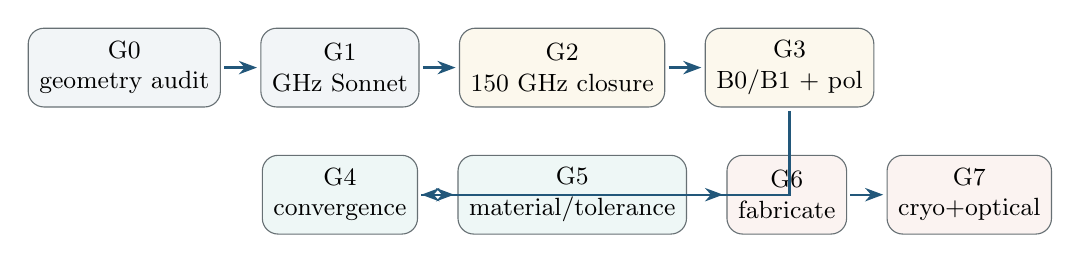
\begin{tikzpicture}[node distance=6mm and 5mm]
\node[flowbox,fill=KidBlue!6] (g0) {G0\\geometry audit};
\node[flowbox,right=of g0,fill=KidBlue!6] (g1) {G1\\GHz Sonnet};
\node[flowbox,right=of g1,fill=KidGold!12] (g2) {G2\\150 GHz closure};
\node[flowbox,right=of g2,fill=KidGold!12] (g3) {G3\\B0/B1 + pol};
\node[flowbox,below=of g1,fill=KidTeal!8] (g4) {G4\\convergence};
\node[flowbox,right=of g4,fill=KidTeal!8] (g5) {G5\\material/tolerance};
\node[flowbox,right=of g5,fill=KidRed!7] (g6) {G6\\fabricate};
\node[flowbox,right=of g6,fill=KidRed!7] (g7) {G7\\cryo+optical};
\draw[flowarrow] (g0) -- (g1);
\draw[flowarrow] (g1) -- (g2);
\draw[flowarrow] (g2) -- (g3);
\draw[flowarrow] (g3.south) |- (g4.east);
\draw[flowarrow] (g4) -- (g5);
\draw[flowarrow] (g5) -- (g6);
\draw[flowarrow] (g6) -- (g7);
\end{tikzpicture}
\end{center}

推荐顺序：
\begin{enumerate}
  \item 冻结 nominal geometry 与 naming；
  \item 完成 GHz resonance/coupler/IDC 层；
  \item 完成 150 GHz single-mode/multi-mode power closure；
  \item 才开始 B0/B1、polarization、angle 主 sweep；
  \item 对最有希望的 2--3 个候选做 convergence；
  \item 再做 material/tolerance；
  \item 只把已经过 gate 的少数设计送加工；
  \item 实验结果回来后反标材料和 geometry，而不是直接“判仿真错”。
\end{enumerate}

\section{一页式 Pre-fabrication Release Checklist}

在提交加工前，下面项目应全部有答案：
\begin{notebookbox}[title=Pre-fabrication release]
\begin{enumerate}
  \item[$\square$] nominal geometry 有唯一版本号和 commit；
  \item[$\square$] X/Y conductor continuity 与 DRC 通过；
  \item[$\square$] GHz $f_0,Q_c$ 与 current map 通过；
  \item[$\square$] 150 GHz TE11-X/Y modal closure 通过；
  \item[$\square$] TM01 已纳入传播模 accounting；
  \item[$\square$] B0/B1 主 FOM 已预先定义；
  \item[$\square$] mesh/frequency convergence 小于 claim margin；
  \item[$\square$] material sensitivity 已检查；
  \item[$\square$] line width / film / backshort / alignment tolerance 已检查；
  \item[$\square$] GDS/CAD 与仿真 geometry 来源一致；
  \item[$\square$] 低温 VNA test plan 已准备；
  \item[$\square$] optical/polarization fixture 能测试论文主 claim。
\end{enumerate}
\end{notebookbox}

\section{一页式 Post-fabrication Closure Checklist}

\begin{notebookbox}[title=Post-fabrication closure]
\begin{enumerate}
  \item[$\square$] measured $f_0,Q_i,Q_c$ 已批量拟合；
  \item[$\square$] measured/simulated frequency shift 有归因；
  \item[$\square$] $f_0(T),Q_i(T)$ 已用于更新材料模型；
  \item[$\square$] optical loading 曲线可重复；
  \item[$\square$] responsivity 与 noise spectrum 使用相同 operating point；
  \item[$\square$] polarization rotation 已得到 X/Y angle 与 leakage；
  \item[$\square$] B0/B1 样品比较使用同一 measurement chain；
  \item[$\square$] 主要偏差没有靠任意 scale factor 掩盖；
  \item[$\square$] 所有论文 figure 可由 raw data + script 重建；
  \item[$\square$] 结论强度与证据等级匹配。
\end{enumerate}
\end{notebookbox}

\section{证据等级：什么结果可以写多强的结论？}

\begin{center}
\noindent\begin{tabularx}{\textwidth}{p{2cm}X X}
\toprule
等级 & 已拥有证据 & 合理措辞 \\
\midrule
E0 & 单一 nominal simulation & ``模型显示/预测……'' \\
E1 & convergence + repeatability & ``数值结果在所测设置下稳定……'' \\
E2 & material + tolerance sensitivity & ``设计优势对主要不确定度稳健……'' \\
E3 & fabricated cryo microwave & ``实物 resonator 参数支持模型……'' \\
E4 & optical/polarization measurement & ``器件实测展示……'' \\
E5 & independent repeat / multi-pixel yield & ``结果具有器件级重复性/可推广性……'' \\
\bottomrule
\end{tabularx}
\end{center}

这张表能避免“E0 证据写成 E4 语气”的过度结论。

\section{最终总图：把所有东西压回一条科研证据链}

\begin{formula}[title=从理论到论文结论]
\[
\boxed{
\begin{aligned}
&\text{BCS / MB / resonator theory}\\
&\Downarrow\\
&\text{parameterized geometry + material model}\\
&\Downarrow\\
&\text{Sonnet GHz verification}\\
&\Downarrow\\
&\text{CST/HFSS optical modal closure}\\
&\Downarrow\\
&\text{B0/B1 + polarization + angle FOM}\\
&\Downarrow\\
&\text{convergence + tolerance + reproducibility}\\
&\Downarrow\\
&\text{fabrication + cryogenic }S_{21}\\
&\Downarrow\\
&\text{optical loading + polarization calibration}\\
&\Downarrow\\
&\text{claim with traceable evidence}
\end{aligned}
}
\]
\end{formula}

\begin{projectbox}
本章的目标不是让读者“多会几个软件”，而是形成一种做 KID 研究时可以复用的习惯：\textbf{先写 claim，再定义 observable；先过数值 gate，再比较设计；先做 uncertainty，再谈 improvement；最后让实验结果反过来更新模型。}
\end{projectbox}

\chapter*{后续版本计划}
\addcontentsline{toc}{chapter}{后续版本计划}
\begin{itemize}
  \item v1.0：阵列与频分复用：resonance placement、collision/yield、readout dynamic range、tone generation/channelization；
  \item v1.1+：RFSoC / FPGA / GPU 实时读出、tone tracking、自动 notch identification、instrument-level calibration 与完整 sensitivity/yield closure。
\end{itemize}

\chapter*{建议参考资料}
\addcontentsline{toc}{chapter}{建议参考资料}
\begin{enumerate}
  \item P. K. Day et al., ``A broadband superconducting detector suitable for use in large arrays,'' \textit{Nature}, 425, 817--821 (2003).
  \item S. Doyle, \textit{Lumped Element Kinetic Inductance Detectors}, PhD thesis, Cardiff University (2008).
  \item J. Zmuidzinas, ``Superconducting Microresonators: Physics and Applications,'' \textit{Annual Review of Condensed Matter Physics}, 3, 169--214 (2012).
  \item J. Gao, \textit{The Physics of Superconducting Microwave Resonators}, PhD thesis, California Institute of Technology (2008).
  \item M. Tinkham, \textit{Introduction to Superconductivity}, 2nd ed., McGraw--Hill (1996).
  \item S. B. Kaplan et al., ``Quasiparticle and phonon lifetimes in superconductors,'' \textit{Physical Review B}, 14, 4854--4873 (1976).
  \item A. Rothwarf and B. N. Taylor, ``Measurement of Recombination Lifetimes in Superconductors,'' \textit{Physical Review Letters}, 19, 27--30 (1967).
  \item P. J. de Visser et al., ``Generation-Recombination Noise: The Fundamental Sensitivity Limit for Kinetic Inductance Detectors,'' \textit{Journal of Low Temperature Physics}, 167, 335--340 (2012).
  \item D. C. Mattis and J. Bardeen, ``Theory of the Anomalous Skin Effect in Normal and Superconducting Metals,'' \textit{Physical Review}, 111, 412--417 (1958).
  \item M. S. Khalil et al., ``An analysis method for asymmetric resonator transmission applied to superconducting devices,'' \textit{Journal of Applied Physics}, 111, 054510 (2012).\\ DOI: \url{https://doi.org/10.1063/1.3692073}.
  \item S. Probst et al., ``Efficient and robust analysis of complex scattering data under noise in microwave resonators,'' \textit{Review of Scientific Instruments}, 86, 024706 (2015).\\ DOI: \url{https://doi.org/10.1063/1.4907935}.
  \item P. J. de Visser et al., ``Evidence of a Nonequilibrium Distribution of Quasiparticles in the Microwave Response of a Superconducting Aluminum Resonator,'' \textit{Physical Review Letters}, 112, 047004 (2014).
  \item P. K. Day et al. and J. Zmuidzinas review sections on optical responsivity and noise are recommended as cross-checks for PSD/NEP conventions.
  \item J. Hubmayr et al., ``Dual-Polarization-Sensitive Kinetic Inductance Detectors for Balloon-borne Sub-millimeter Polarimetry,'' \textit{Journal of Low Temperature Physics}, 176, 490--496 (2014), doi:10.1007/s10909-014-1160-2.
  \item H. McCarrick et al., ``Development of dual-polarization LEKIDs for CMB observations,'' Proc. SPIE / arXiv:1607.03448 (2016).
  \item H. McCarrick et al., ``Design and performance of dual-polarization lumped-element kinetic inductance detectors for millimeter-wave polarimetry,'' \textit{Astronomy \& Astrophysics}, 610, A45 (2018), arXiv:1710.02239.
\end{enumerate}

\end{document}
